\documentclass[xcolor=dvipsnames,10pt]{beamer}
% ********** Styl prezentacji **********
\mode<presentation>
{
%\usetheme{Frankfurt}
%\usetheme{Copenhagen}
\usetheme{Madrid}
 %\usetheme{lankton-keynote}
 %Copenhagen
}
%\usepackage{amsmath}
%\usepackage{amsthm}
%\usepackage{amsfonts}
\usepackage{color}
%\usepackage{listings}
%\lstset{language=C++}
%\usepackage{lscape} 
%\usepackage{float}
%\usepackage{graphicx}
\usepackage{caption}
\usepackage{subcaption}
%\usepackage{multimedia}
% common reference commands
\renewcommand{\Re}{\textrm{Re}}
\newcommand{\Pe}{\textrm{P\'e}}
\renewcommand{\Pr}{\textrm{Pr}}
\newcommand{\eqt}[1]{Eq.~(\ref{#1})}                     % equation
\newcommand{\fig}[1]{Fig.~\ref{#1}}                      % figure
\newcommand{\tbl}[1]{Table~\ref{#1}}                     % table
%\usepackage{movie15}
%\usepackage{hyperref}
%\usepackage{multimedia}
\usepackage[]{media9}
%\usepackage{filecontents,hyperref,listings}
\newcommand{\resi}{R}
\newcommand{\resinew}{\widetilde{\resi}}
\newcommand{\resisource}{\widetilde{\resi}^{source}}
\renewcommand{\div}{\vec{\nabla}\! \cdot \!}
\newcommand{\grad}{\vec{\nabla}}
\newcommand{\divv}[1]{\vec{\nabla}^{#1}\! \cdot \!}
\newcommand{\gradd}[1]{\vec{\nabla}^{#1}}
\newcommand{\mbold}[1]{\boldsymbol#1}
\newcommand{\norm}{\textrm{norm}}
%

\newcommand{\tcr}[1]{\textcolor{red}{#1}}

%\setbeamertemplate{footline}[frame number]
%\title{Extension of the entropy viscosity method to low Mach regime and the seven equations model.}
%\title{Extension of the entropy viscosity method to low Mach regime and the seven equations model.}
%\author{Marc-Olivier Delchini}
%
\begin{document}
%
%\begin{frame}
%\maketitle
%\end{frame}
\begin{frame}
\begin{center}
Extension of the entropy viscosity method to the low Mach multi-D Euler equations and the seven-equation model.
\begin{center}
by \\
Marc-Olivier Delchini
\end{center}
\today \\

Co-chairs: J. Ragusa\footnote{Nuclear Engineering Department, Texas A\&M University.} and J.L. Guermond\footnote{Department of Mathematics, Texas A\&M University.}. \\
Committee members: J. Morel\footnotemark[1], Y. Hassan\footnotemark[1] and R. Berry\footnote{Idaho National Laboratory.}. \\
Substitute: R. McClarren
\end{center}
\end{frame}
%
\begin{frame}
	\frametitle{Outline:}
	\tableofcontents
\end{frame}
%************************************************
\section{Introduction}
\begin{frame}{Introduction}
\emph{Why do we need to solve for conservation laws?}
\begin{block}{}
\begin{itemize}
\setlength{\itemsep}{10pt}
\item Hyperbolic conservation laws $\longrightarrow$ nuclear engineering, aeronautic, aerospace, oil engineering, $\dots$
\item Systems of equations that accurately describe the physical phenomena
\item Need for accurate and robust modeling for engineering applications
\item Require good understanding of the mathematical properties (eigenvalues, characteristic equations and variables , shock formation, $\dots$ )
\item Numerical stabilizations: approximate Riemann solvers (HLL, HLLC), flux limiters, artificial dissipative methods, $\dots$
\end{itemize}
\end{block}
\end{frame}
%************************************************
\begin{frame}{Some mathematical properties}
%\tcr{consistency issue: use vector or bold but do not mix them}
Let us consider a hyperbolic conservation law of the form:
\begin{equation} \partial_t \vec{U} + \div \vec{F} ( \vec{U} ) = \vec{0}  \nonumber \text{ (strong form)}\end{equation} 
\begin{itemize}
\item wave-dominated problem $\to$ eigenvalues
\item known to form shocks even with smooth initial conditions: characteristic equations and variables, Riemann invariants
\item uniqueness of the weak solution is ensured by an \textbf{\emph{entropy condition}}: the associated entropy equation satisfies an inequality and is \emph{peaked in the shock region}.
\begin{equation}
\partial_t S ( \vec{U} ) + \div \vec{\Psi} ( \vec{U} ) \geq 0 \text{ entropy inequality} \nonumber
\end{equation}
%\tcr{this reads a grad of psi but it should be div of vector psi}
$S$: physical entropy \\
$\left( S, \Psi \right)$ is an entropy pair
\end{itemize}
\end{frame}
%************************************************
\begin{frame}{The general idea behind the entropy viscosity method}
\emph{It is an artificial dissipation method with smart viscosity coefficient(s)  capable of tracking the shock so that dissipation is only added into the shock region.}
\begin{block}{}
\begin{itemize}
\setlength{\itemsep}{10pt}
\item it is a viscous regularization technique: the dissipative terms are consistent with the entropy inequality. 
%\tcr{why requires? why not ``is a viscous regularization technique''?\\} \tcr{entropy inequality is vague and not yet defined}
\item each viscosity coefficient is function of a high-order viscosity coefficient and an upper bound called first-order viscosity coefficient.
\item the high-order viscosity coefficient is defined proportional to the entropy residual.
\item the first-order viscosity coefficient is function of the local maximum eigenvalue.
\item also accounts for the inter element jumps $\to$ make the definition of the viscosity coefficients also sensitive to all discontinuities. 
\end{itemize}
\end{block}
\end{frame}
%************************************************
\begin{frame}{The Multiphysics Object-Oriented Simulations Environment (MOOSE)}
\begin{block}{}
\begin{itemize}
\setlength{\itemsep}{10pt}
\item Explicit and implicit temporal integrators (first and second-order accuracy)
\item Continuous and Discontinuous Galerkin Finite Element Method
\item Mesh adaptivity, time step adaptivity
\item Support parallel runs
\item Buildt on PETSc and Libmesh
\item For implicit solve, requires a preconditioner $\to$ either Finite Difference Preconditioner (FDP) 
%\tcr{acronym not defined} 
or hard-coded preconditioner
\item C++ language, open-source
\end{itemize}
\end{block}
\begin{block}{}
All numerical solutions were run with BDF2 and linear test functions $\to$ second-order accuracy in time and space for smooth solutions only!.
\end{block}
\end{frame}
%************************************************
\begin{frame}
\begin{center}
BurGer's Equation \\
(BadGEr)
\end{center}
\begin{figure}[H]
\centering
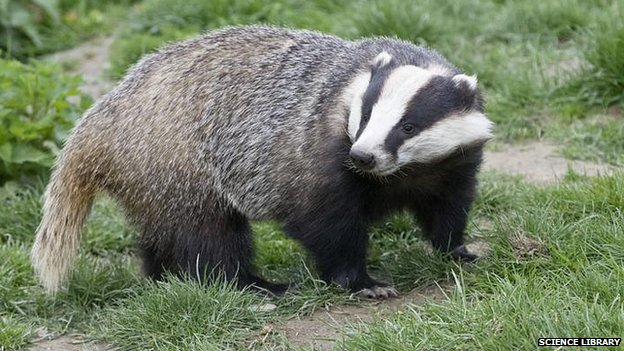
\includegraphics[width=0.5\textwidth]{../figures/badger.png}
\end{figure}
\end{frame}
%************************************************
\begin{frame}{A simple example of application of the EVM: the $1$-D Burger's equation}
\begin{block}{The $1$-D Burger's equation with its viscous regularization}
\begin{equation}
\partial_t u(x,t) + \partial_x \left( \frac{u(x,t)^2}{2} \right) = \textcolor{blue}{\partial_x \left( \mu \left(x,t \right) \partial_x u(x,t) \right)} \nonumber
\end{equation}
\end{block}
\begin{block}{Definition of the local viscosity coefficient $\mu(x,t)$}
\begin{align}
&\mu(x,t) = \min \left( \mu_e(x,t), \mu_{max}(x,t) \right) \nonumber \\
&\mu_{max} (x,t) = \frac{h}{2} | u(x,t) | \nonumber \\
&\mu_e(x,t) = h^2 \frac{\max \left( R(x,t), J \right)}{|| \eta(u) - \bar{\eta}(t) ||_\infty} \nonumber \\
& \text{Entropy residual: }R(x,t) = \partial_t \eta(u) + \partial_x \Phi(u) \leq 0 \text{ with } \eta(u) = u^2 / 2 \nonumber \\
\text{ and } \Phi(u) = u^3 / 3 \nonumber \\
&\text{Jump: } J = [[ \partial_x \Phi(u) ]] \nonumber
\end{align}
\tcr{phi not defined}
\end{block}
\end{frame}
%************************************************
\begin{frame}{$1$-D numerical results (100 cells and CFL $=1$)}
\begin{figure}[H]
        \centering
        \begin{subfigure}[b]{0.37\textwidth}
                \centering
                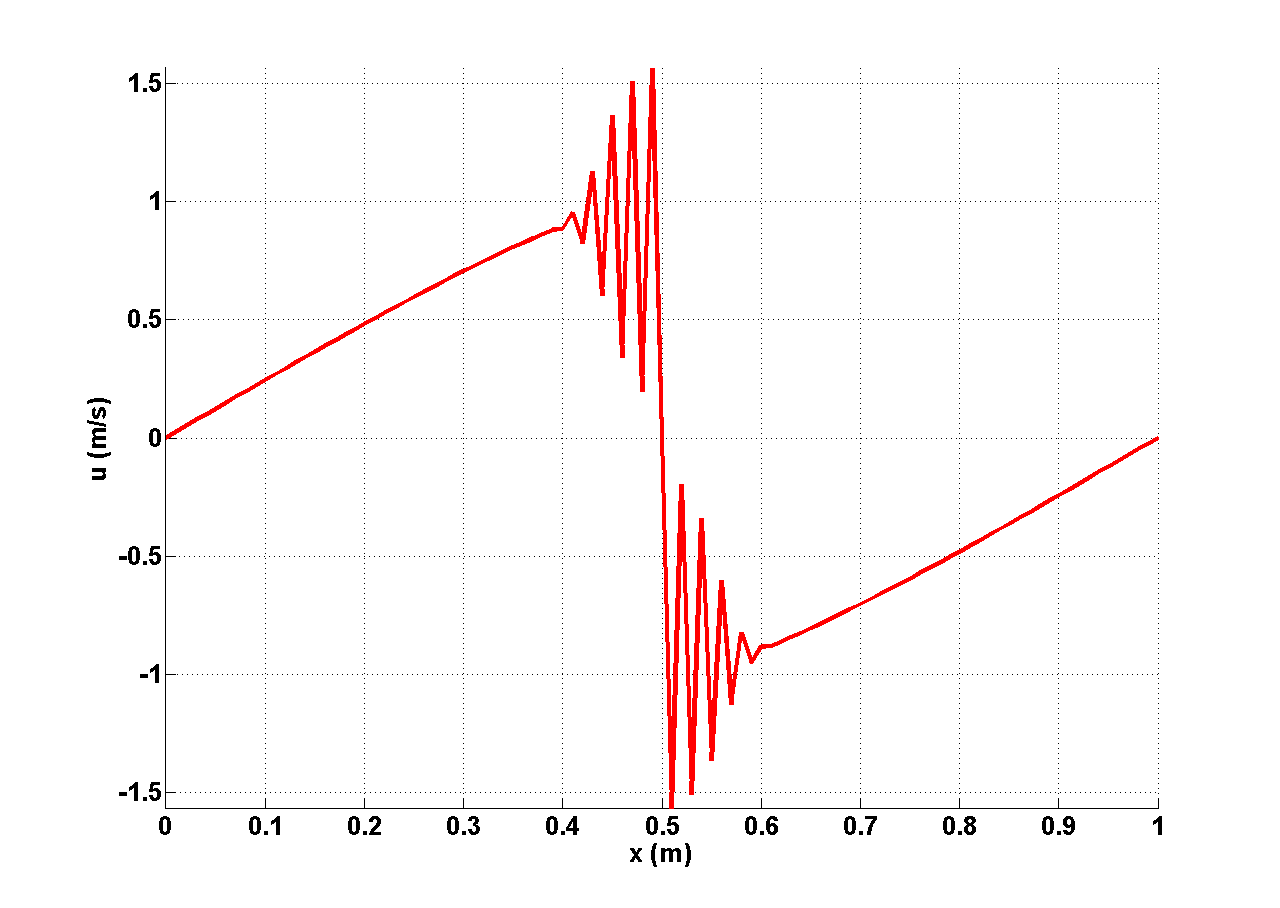
\includegraphics[width=\textwidth]{../figures/1D_sol_free.png}
                \caption{Without stabilization.}
        \end{subfigure}%
        \begin{subfigure}[b]{0.37\textwidth}
                \centering
                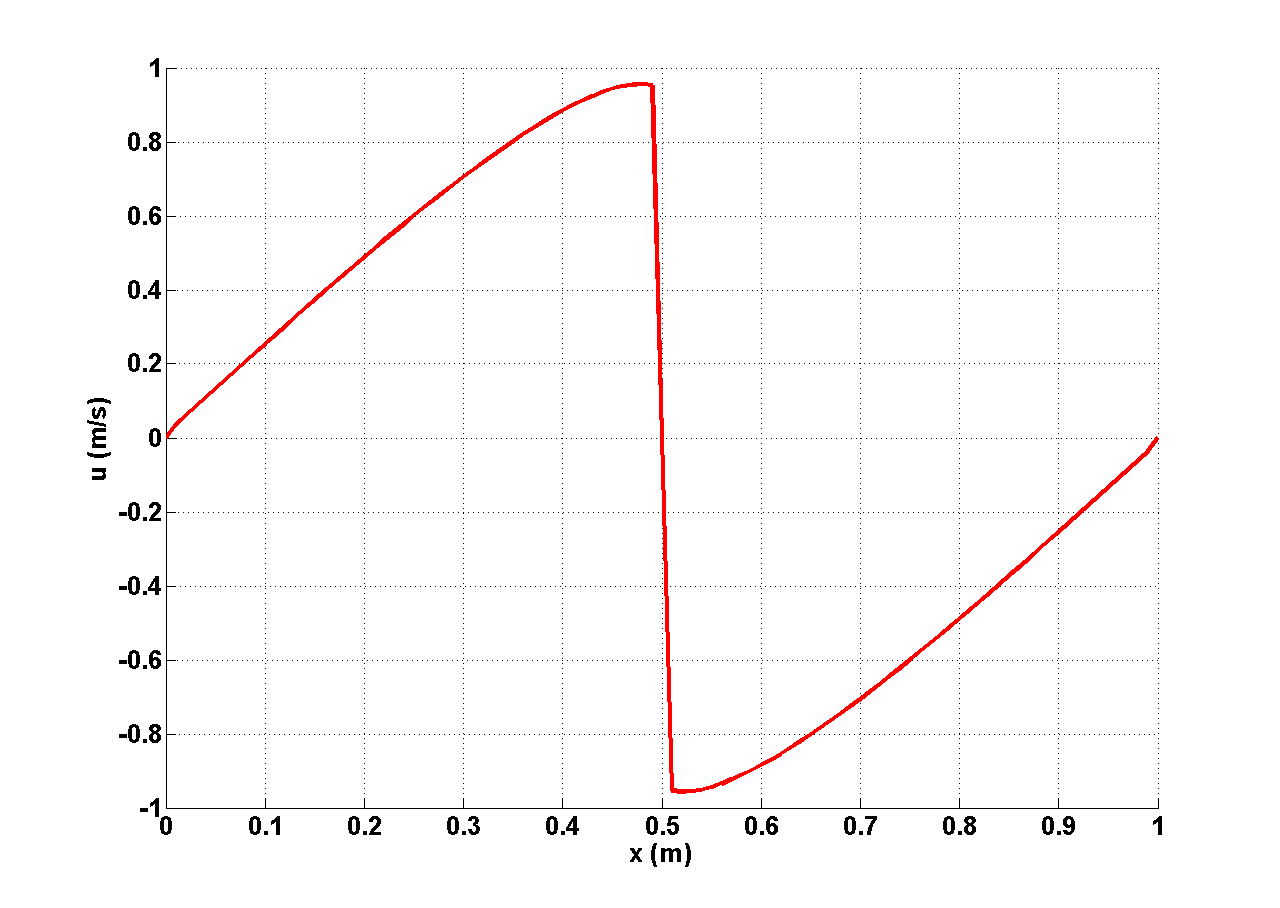
\includegraphics[width=\textwidth]{../figures/1D_sol_fo.png}
                \caption{With first-order viscosity.}
        \end{subfigure}
        
        \begin{subfigure}[b]{0.37\textwidth}
                \centering
                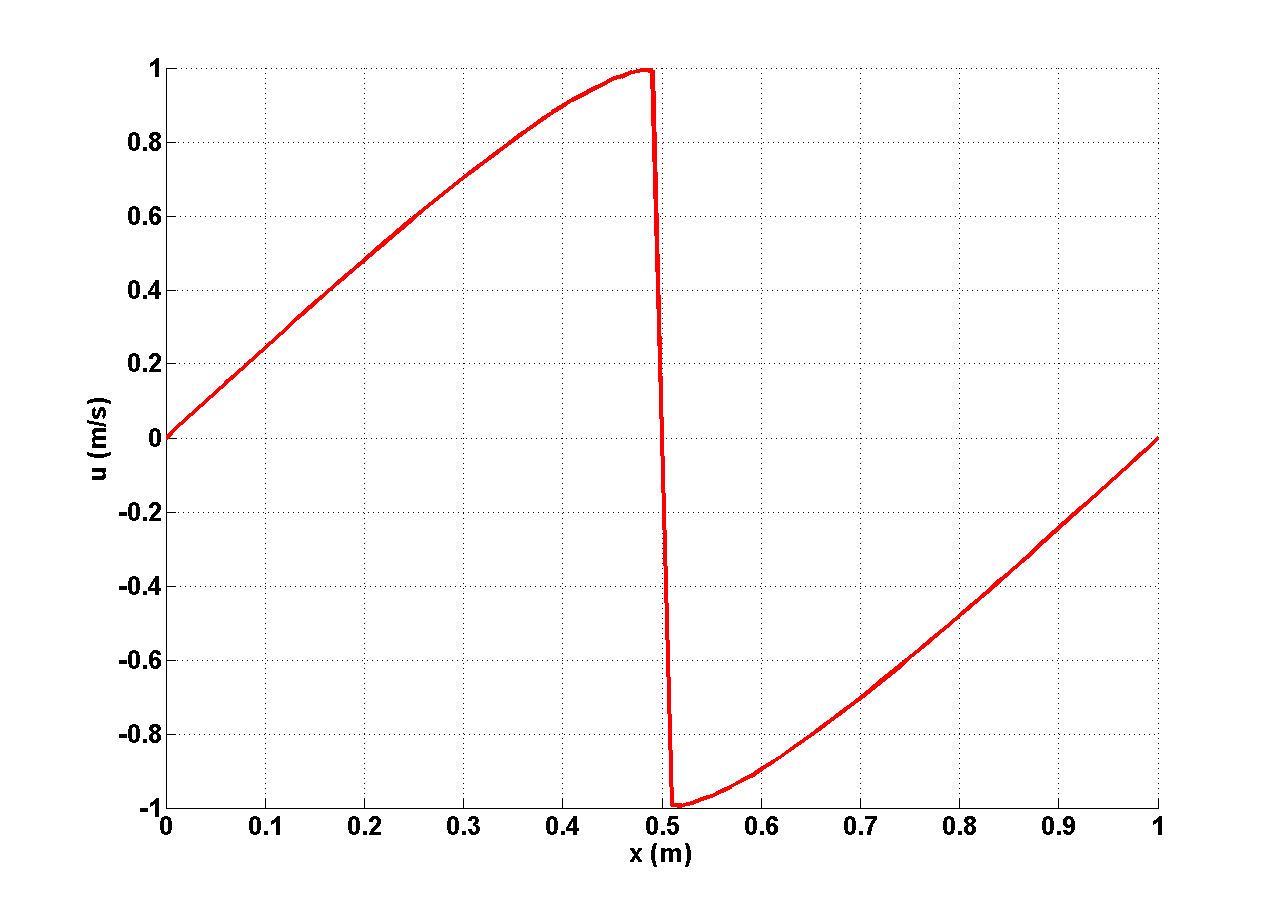
\includegraphics[width=\textwidth]{../figures/1D_sol_ev.png}
                \caption{With the EVM.}
        \end{subfigure}
        \begin{subfigure}[b]{0.37\textwidth}
                \centering
                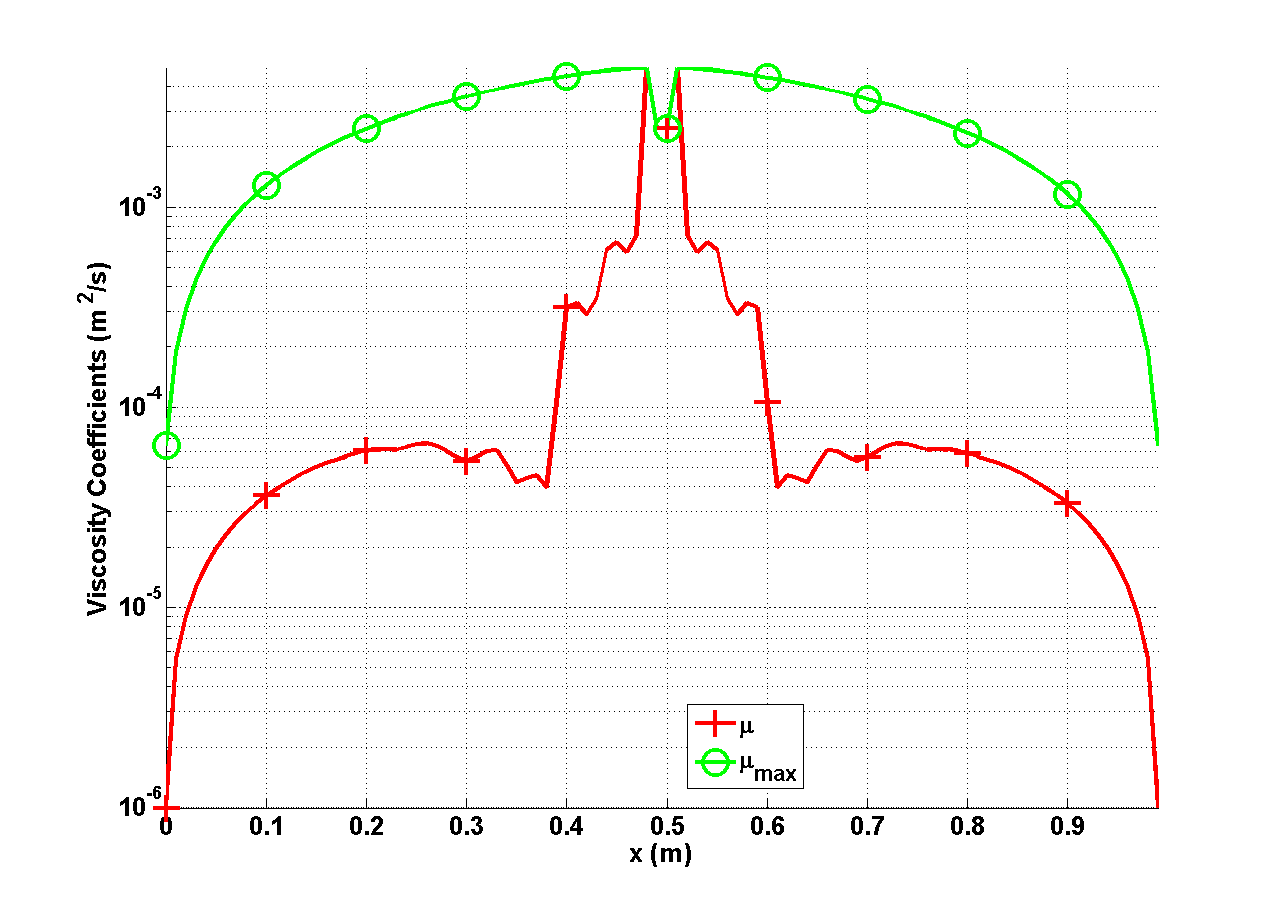
\includegraphics[width=\textwidth]{../figures/1D_visc.png}
                \caption{Viscosity coefficient profiles.}
        \end{subfigure}
\end{figure}
\end{frame}
%************************************************
\section{The multi-D Euler equations with variable area}
\begin{frame}
\begin{center}
The MULti-D Euler Equations with variable area \\
(MULe DEEr)
\end{center}
\begin{figure}[H]
\centering
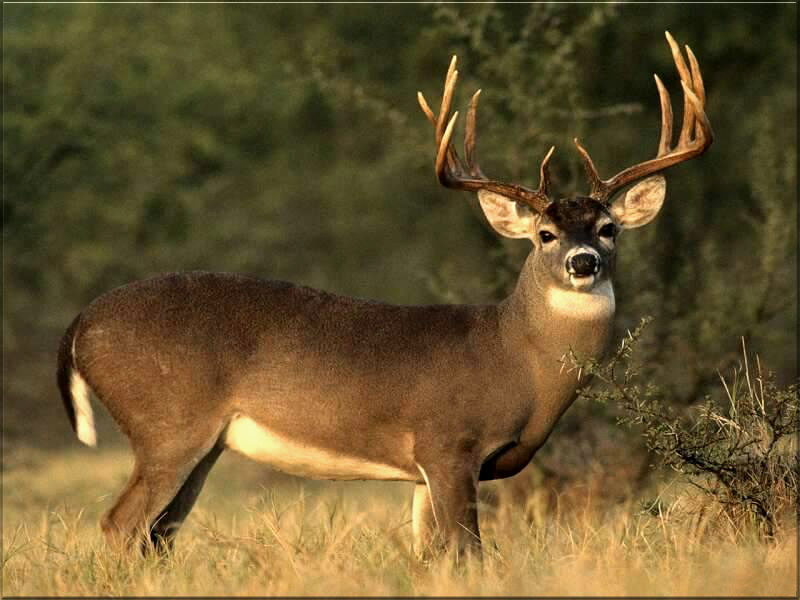
\includegraphics[width=0.5\textwidth]{../figures/Mule_Deer.png}
\end{figure}
\end{frame}
%************************************************
\begin{frame}
\begin{block}{Numerical methods for continuous and discontinuous schemes}
\begin{itemize}
\setlength{\itemsep}{10pt}
\item multi-wave problem, can develop shock waves and other types of discontinuities. 
\item Numerical methods for both continuous and discontinuous schemes: approximate Riemann solvers (HLL, HLLC, Roe scheme, $\cdots$), flux limiters
, Lapidus viscosity, Pressure-based viscosity, SUPG, C-method, Entropy Viscosity Method (EVM). 
\item Numerical method can be ill-scaled in the low-Mach limit, yielding the wrong incompressible system $\to$ use of a Mach-based preconditioner for the dissipative terms to obtain the correct behavior in the low-Mach limit.
\item Low-Mach steady-state solution: time-dependent term preconditioner to accelerate the convergence of the solution to the steady-state (Turkel) when using an explicit scheme $\to$ the transient is no longer accurate. \emph{Implicit solvers do not have this issue}. 
\end{itemize}
\end{block}
\end{frame}
%************************************************
\begin{frame}
\begin{block}{}
%\tcr{vector consistency issue}
\begin{itemize}
\setlength{\itemsep}{10pt}
\item The isentropic compressible multi-D Euler equations degenerate into an incompressible system in the low-Mach asymptotic limit.
\begin{align}
&\partial_t \rho + \vec{u} \cdot \grad \rho = 0 \nonumber \\
&\partial_t \vec{u} + \vec{u}\text{ } \div \vec{u} + \frac{1}{\rho}\grad P = 0 \nonumber \\
& \div \vec{u} = 0 \nonumber \\
&P( \vec{r},t) = P_0(t) + M^2 P_2(\vec{r},t)\nonumber
\end{align}
$\to$ no energy equation since the flow is assumed isentropic \\
$\to$ pressure fluctuations of the order of the Mach number square \emph{at steady state}% \tcr{isn't that only at steady state?}
\end{itemize}
\end{block}
\end{frame}
%************************************************
\begin{frame}
\begin{block}{The multi-D Euler equations with variable area}
%\tcr{fix alignment; it looks out of whack; maybe use subequations with the text in between the equations}
\begin{subequations}
Mass conservation
\begin{align}
&\partial_t ( \rho A ) + \div \left( \rho A \vec{u} \right) = 0 \nonumber
\end{align}
Momentum conservation
\begin{align}
&\partial_t ( \rho \vec{u} A ) + \div \left( \rho A \vec{u} \otimes \vec{u} + P \mathbb{I} \right) = P \grad A \nonumber
\end{align}
Energy conservation
\begin{align}
&\partial_t ( \rho E A ) + \div \left[ \vec{u} \left( \rho E + P \right) A \right] = 0 \nonumber
\end{align}
Equation of state
\begin{align}
& P = eos \left( \rho, e \right) \nonumber 
\end{align}
\end{subequations}
\end{block}
Multi-wave problem: $\lambda_1 = \vec{u} \cdot \vec{n} - c $, $\lambda_2 = \vec{u} \cdot \vec{n} + c $ and $\lambda_{3, \dots, 3+D} = \vec{u} \cdot \vec{n}$. \\
The area $A$ is only a function of space.
\end{frame}
%************************************************
\begin{frame}
\emph{Objectives: extend the EVM to low-Mach flows while maintaining its capabilities of solving for transonic and supersonic flows, and use an implicit solver.}
\begin{block}{How to do it?}
\begin{enumerate}
\setlength{\itemsep}{10pt}
\item recast the entropy equation as a function of the pressure, the density, the velocity and the speed of sound.
\item derive a viscous regularization for the multi-D Euler equations (Guermond and Popov (2014)) $\rightarrow$ extended to Euler equation with variable area.
\item work with the non-dimensionalized version of the multi-D Euler equations in order to understand how the different terms scale $\to$ will define non-dimensionalized numbers (Mach number, numerical Reynolds number, $\dots$)
\item derive a definition for the viscosity coefficients that ensures well-scaled dissipative terms for a wide range of Mach numbers $\to$ will consider two cases: isentropic and non-isentropic (with shocks) flows.
\end{enumerate}
\end{block}
\end{frame}
%************************************************
\begin{frame}{Recast the entropy residual}
\begin{block}{New entropy residual}
\begin{equation}
D_e(\vec{r},t) = \partial_t s + \vec{u} \cdot \grad s = \frac{s_e}{P_e} \underbrace{\left( \frac{d P}{dt} - c^2 \frac{d \rho}{dt} \right)}_{\tilde{D}_e(\vec{r},t)} \nonumber
\end{equation}
\end{block}
\begin{block}{The viscosity coefficients}
\begin{itemize}
\item The viscosity coefficient will be set proportional to $\tilde{D}_e(\vec{r},t)$ (instead of $D_e(\vec{r},t)$):
\begin{equation}
\mu_e(\vec{r},t) = h^2 \frac{\max \left( \tilde{D}_e(\vec{r},t), J \right)}{\norm_P^\mu} \text{ and }\kappa_e(\vec{r},t) = h^2 \frac{\max \left( \tilde{D}_e(\vec{r},t), J \right)}{\norm_P^\kappa} \nonumber
\end{equation}
\item $\tilde{D}_e(\vec{r},t)$ is an alternative way of computing the local entropy production
\item This new expression offers more diversity in the choice of the \textbf{normalization parameter} $norm_P$: $P$, $\rho c^2$, $\rho c ||\vec{u} ||$ or  $\rho ||\vec{u}||^2$
\end{itemize}
\end{block}
\end{frame}
%************************************************
\begin{frame}{A viscous regularization for the multi-D Euler equations with variable area}
\begin{align}
&\text{Mass conservation} \nonumber \\
&\partial_t ( \rho A ) + \div \left( \rho A \vec{u} \right) = \textcolor{blue}{\div \vec{f}} \nonumber \\
&\text{Momentum conservation} \nonumber \\
&\partial_t ( \rho \vec{u} A ) + \div \left( \rho A \vec{u} \otimes \vec{u} + P \mathbb{I} \right) = P \grad A + \textcolor{blue}{\div \left( \mathbb{F}(\vec{u}) + \vec{u} \otimes \vec{f} \right)} \nonumber \\
&\text{Energy conservation} \nonumber \\
&\partial_t ( \rho E A ) + \div \left[ \vec{u} \left( \rho E + P \right) A \right] = \textcolor{blue}{\div \left( \vec{h} + \vec{u}\cdot \mathbb{F}(\vec{u}) + \frac{|| \vec{u} ||^2}{2} f \right)} \nonumber \\
&\text{Dissipative terms} \nonumber \\
& \textcolor{blue}{\vec{f} = A \kappa \grad \rho \text{, } \vec{h} = A \kappa \grad ( \rho e) } \nonumber
\text{ and } \textcolor{blue}{\mathbb{F}(\vec{u}) = A \mu \grad^s \vec{u}} \text{ or } \textcolor{blue}{\mathbb{F}(\vec{u}) = A \mu \grad \vec{u}}
\end{align}
$\to$ two positive viscosity coefficients $\mu$ and $\kappa$. Requires a concave physical entropy $s(\rho,e)$.
\end{frame}
%************************************************
\begin{frame}{Non-dimensionalized multi-D Euler equations}
We define some reference variables denoted by subscript $\infty$:
\begin{multline}
\rho^*   = \frac{\rho}{\rho_\infty}           ,\
u^*      = \frac{u}{u_\infty}                 ,\
P^*      = \frac{P}{\rho_\infty c^2_\infty}   ,\
E^*      = \frac{E}{c^2_\infty }              ,\\
x^* = \frac{x}{L_\infty}                      ,\
t^* = \frac{t}{L_\infty / u_\infty}           ,\ 
\textcolor{blue}{\mu^*    = \frac{\mu}{\mu_\infty}}             ,\
\textcolor{blue}{\kappa^* = \frac{\kappa}{\kappa_\infty}}     \nonumber
\end{multline}
$\to$ $\mu_\infty$ and $\kappa_\infty$ are function of the normalization parameters $norm_P^\mu$ and $norm_P^\kappa$, respectively.
We also define the following reference numbers:
\begin{align}
&\text{Mach number: }M_\infty = \frac{u_\infty}{c_\infty}, \nonumber\\
&\text{Numerical Reynolds number: }\Re_\infty = \frac{u_\infty L_\infty}{\textcolor{blue}{\mu_\infty}} , \nonumber \\
&\text{Numerical P\'echlet number: }\Pe_\infty = \frac{u_\infty L_\infty}{\textcolor{blue}{\kappa_\infty}} , \nonumber \\
&\text{Numerical Prandlt number: }\Pr_\infty = \Pe_\infty / \Re_\infty = \mu_\infty / \kappa_\infty \nonumber \nonumber
\end{align}
\end{frame}
%************************************************
\begin{frame}{Non-dimensionalized multi-D Euler equations}
\begin{subequations} 
%
\begin{equation}
\partial_{t^*} \rho^*+ \divv{*}  \left(  \rho^* \vec{u}^*  \right) = \textcolor{blue}{\frac{1}{\Pe_\infty} \divv{*}  ( \kappa^* \gradd{*} \rho^* )} \nonumber
\end{equation}
%
\begin{align}
\partial_{t^*} \left( \rho^* \vec{u}^* \right) 
+ \divv{*} \left( \rho^* \vec{u}^*\otimes \vec{u}^* \right) 
+ \textcolor{magenta}{\frac{1}{M_\infty^2}\gradd{*}  P^*}  
&= 
\textcolor{blue}{\frac{1}{\Re_\infty} \divv{*} \left( \rho^* \mu^* \gradd{s,*} \vec{u}^* \right)}  \nonumber\\
&+
\textcolor{blue}{\frac{1}{\Pe_\infty} \divv{*} \left(\vec{u}^*\otimes \kappa^* \gradd{*}  \rho^* \right)} \nonumber
\end{align}
%
\begin{align}
\partial_{t^*} \left( \rho^* E^* \right) 
+ \divv{*}  \left[ \vec{u}^* \left( \rho^* E^* + P^* \right) \right] 
&=
\textcolor{blue}{\frac{1}{\Pe_\infty} \divv{*}  \left( \kappa^*  \gradd{*} (\rho^* e^*) \right)} \nonumber  \\
+
\textcolor{blue}{\frac{M_\infty^2}{\Re_\infty} \divv{*}  \left( \vec{u}^* \rho^* \mu^* \gradd{s,*} \vec{u}^* \right)}
&+ 
\textcolor{blue}{\frac{M_\infty^2}{2 \Pe_\infty} \divv{*}  \left(\kappa^* (u^*)^2 \gradd{*} \rho^* \right)} \nonumber
\end{align}
%
\end{subequations}
The above equations are valid for both isentropic and non-isentropic flows and for all Mach numbers.
\end{frame}
%************************************************
\begin{frame}{For an isentropic flow}
$\to$ choose $\Re_\infty$ and $\Pe_\infty$ so that we recover the incompressible equations in the low-Mach limit.
\begin{block}{}
\begin{itemize}
\setlength{\itemsep}{10pt}
\item assume Ideal gas equation of state for simplicity: $P = ( \gamma-1) \rho e$
\item choose $\Re_\infty = \Pe_\infty = 1$
\item expand each variable in powers of the Mach number: $P(\vec{r}, t) = P_0(\vec{r}, t) + P_1(\vec{r}, t) M_\infty + P_2(\vec{r}, t) M_\infty^2 + \dots $
\item derive the leading, first and second-order momentum equations
\item derive the leading-order energy and mass equations
\end{itemize}
\end{block}
\end{frame}
%************************************************
\begin{frame}{For an isentropic flow: momentum equation}
\begin{align}
\partial_{t} \left( \rho \vec{u} \right) 
+ \div \left( \rho \vec{u}\otimes \vec{u} \right) 
+ \textcolor{magenta}{\frac{1}{M_\infty^2}\grad  P}
&= 
\textcolor{blue}{\frac{1}{\Re_\infty} \div \left( \rho \mu \gradd{s} \vec{u} \right)}
&+
\textcolor{blue}{\frac{1}{\Pe_\infty} \div \left(\vec{u}\otimes \kappa \grad  \rho \right)} \nonumber
\end{align}
\begin{block}{}
Leading and first-order momentum equations:
\begin{align}
&\grad P_0 = \grad P_1 = 0 \longrightarrow P(\vec{r}, t) = \tilde{P}_0(t) + P_2(\vec{r}, t) M_\infty^2\nonumber 
\end{align}
Second-order momentum equation:
\begin{align}
&\partial_t (\rho \vec{u} )_0 + \div \left( \rho \vec{u}\otimes \vec{u} \right)_0 + \textcolor{magenta}{P_2} = \textcolor{blue}{ \div \left( \rho \mu \gradd{s} \vec{u} \right)_0}
+
\textcolor{blue}{ \div \left(\vec{u}\otimes \kappa \grad  \rho \right)_0} \nonumber
\end{align}
\end{block}
\end{frame}
%************************************************
\begin{frame}{For an isentropic flow: energy and mass equations}
\begin{align}
\partial_{t^*} \left( \rho^* E^* \right) 
+ \divv{*}  \left[ \vec{u}^* \left( \rho^* E^* + P^* \right) \right] 
&=
\textcolor{blue}{\frac{1}{\Pe_\infty} \divv{*}  \left( \kappa^*  \gradd{*} (\rho^* e^*) \right)} \nonumber \\
+
\textcolor{blue}{\frac{M_\infty^2}{\Re_\infty} \divv{*}  \left( \vec{u}^* \rho^* \mu^* \gradd{s,*} \vec{u}^* \right)}
&+ 
\textcolor{blue}{\frac{M_\infty^2}{2 \Pe_\infty} \divv{*}  \left(\kappa^* (u^*)^2 \gradd{*} \rho^* \right)} \nonumber
\end{align}
\begin{block}{}
Leading-order energy equation:
\begin{align}
\partial_t ( \rho E )_0 + \div \left[ \vec{u} \left( \rho E + P \right) \right]_0 = \textcolor{blue}{\div \left( \kappa  \grad (\rho e) \right)_0} \longrightarrow \div \vec{u}_0 = 0 \nonumber 
\end{align}
\end{block}
\begin{align}
\partial_{t} \rho+ \div  \left(  \rho \vec{u}  \right) = \textcolor{blue}{\frac{1}{\Pe_\infty} \div  ( \kappa \grad \rho )} \nonumber
\end{align}
\begin{block}{}
Leading-order mass equation:
\begin{align}
\partial_{t} \rho_0+ \div  \left(  \rho \vec{u}  \right)_0 = \textcolor{blue}{ \div ( \kappa \grad \rho )_0} \to \partial_t \rho_0 + \vec{u}_0 \grad \rho_0 = \textcolor{blue}{ \div ( \kappa \grad \rho )_0}\nonumber
\end{align}
\end{block}
\end{frame}
%************************************************
\begin{frame}{For an isentropic flow: derivation of $\norm_P^{\mu, \kappa}$ }
We were able to recover the incompressible equations by choosing $\Re_\infty = \Pe_\infty = 1$. What does that imply for $\norm_P^\mu$ and $\norm_P^\kappa$?
\begin{block}{}
Derive an expression for $\kappa_\infty$:
\begin{align}
&\kappa_e(\vec{r},t) = h^2 \frac{\max \left( \tilde{D}_e(\vec{r},t), J \right)}{\norm_P^\kappa} \longrightarrow \kappa_\infty = \frac{ \rho_\infty c_\infty^2 u_\infty L }{ \norm_{P,\infty}^\kappa } \nonumber 
\end{align}
Then, use the substitute the above expression for $\norm_P^\kappa$ into $\Pe_\infty$ to obtain:
\begin{align}
&\norm_{P,\infty}^{\kappa} = \Pe_\infty \rho_\infty c_\infty^2 = \rho_\infty c_\infty^2 \nonumber
\end{align}
\end{block}
\begin{block}{}
Same derivation using $\mu_e$ and $\Re_\infty$ leads to:
\begin{align}
\norm_{P,\infty}^{\mu} = \Re_\infty \rho_\infty c_\infty^2 = \rho_\infty c_\infty^2 \nonumber
\end{align}
\end{block}
\end{frame}
%************************************************
\begin{frame}{For a non-isentropic flow, i.e., with shocks}
\begin{block}{}
\begin{itemize}
\setlength{\itemsep}{10pt}
\item the flow can experience shocks and other waves $\to$ discontinuities
\item the low-Mach asymptotic study is no longer valid
\item directly work with the non-dimensionalized Euler equations
\item determine the scaling of $\Re_\infty$ and $\Pe_\infty$ to stabilize the equations
\item look at the low-Mach limit
\end{itemize}
\end{block}
\end{frame}
%************************************************
\begin{frame}{For a non-isentropic flow: momentum equation}
\begin{align}
\partial_{t} \left( \rho \vec{u} \right) 
+ \div \left( \rho^* \vec{u}\otimes \vec{u} \right) 
+ \textcolor{magenta}{\frac{1}{M_\infty^2}\grad  P}  
= 
\textcolor{blue}{\frac{1}{\Re_\infty} \div \left( \rho \mu \gradd{s} \vec{u} \right)} +
\textcolor{blue}{\frac{1}{\Pe_\infty} \div \left(\vec{u}\otimes \kappa \grad  \rho \right)} \nonumber
\end{align}
\begin{block}{}
In the shock region, the term $\textcolor{magenta}{\frac{1}{M_\infty^2}\grad  P}  $ will become dominant and will need to be stabilize by a dissipative term of the same scaling:
\begin{itemize}
\setlength{\itemsep}{10pt}
\item (a) $\Re_\infty = M_\infty^2$ and $\Pe_\infty = 1$
\item (b) $\Re_\infty = 1$ and $\Pe_\infty = M_\infty^2$
\item (c) $\Re_\infty = \Pe_\infty = M_\infty^2$
\end{itemize}
$\longrightarrow$ each of the above options will affect the other equations (mass and energy equations).
\end{block}
\end{frame}
%************************************************
\begin{frame}{For a non-isentropic flow: mass equation}
\begin{equation}
\partial_{t} \rho+ \div  \left(  \rho \vec{u}  \right) = \textcolor{blue}{\frac{1}{\Pe_\infty} \div  ( \kappa \grad \rho )} \nonumber
\end{equation}
\begin{block}{choice (a) $\Pe_\infty = 1$}
\begin{equation}
\partial_{t} \rho+ \div  \left(  \rho \vec{u}  \right) = \textcolor{blue}{\div  ( \kappa \grad \rho )} \nonumber
\end{equation}
$\to$ the dissipative term is \emph{well-scaled}
\end{block}
\begin{block}{choice (b) and (c) $\Pe_\infty = M_\infty^2$}
\begin{equation}
\partial_{t} \rho+ \div  \left(  \rho \vec{u}  \right) = \textcolor{blue}{\frac{1}{M_\infty^2} \div  ( \kappa \grad \rho )} \nonumber
\end{equation}
$\to$ the dissipative term is \emph{ill-scaled}
\end{block}
Options (b) and (c) are not inappropriate. Thus, we are left with option (a): $\Re_\infty = M_\infty^2$ and $\Pe_\infty = 1$
\end{frame}
%************************************************
\begin{frame}{For a non-isentropic flow: energy equation}
\begin{align}
\partial_{t^*} \left( \rho^* E^* \right) 
+ \divv{*}  \left[ \vec{u}^* \left( \rho^* E^* + P^* \right) \right] 
&=
\textcolor{blue}{\frac{1}{\Pe_\infty} \divv{*}  \left( \kappa^*  \gradd{*} (\rho^* e^*) \right)} \nonumber  \\
+
\textcolor{blue}{\frac{M_\infty^2}{\Re_\infty} \divv{*}  \left( \vec{u}^* \rho^* \mu^* \gradd{s,*} \vec{u}^* \right)}
&+ 
\textcolor{blue}{\frac{M_\infty^2}{2 \Pe_\infty} \divv{*}  \left(\kappa^* (u^*)^2 \gradd{*} \rho^* \right)} \nonumber
\end{align}
\begin{block}{With option (a) it yields:}
\begin{align}
\partial_{t^*} \left( \rho^* E^* \right) 
+ \divv{*}  \left[ \vec{u}^* \left( \rho^* E^* + P^* \right) \right] 
&=
\textcolor{blue}{ \divv{*}  \left( \kappa^*  \gradd{*} (\rho^* e^*) \right)} \nonumber  \\
+
\textcolor{blue}{ \divv{*}  \left( \vec{u}^* \rho^* \mu^* \gradd{s,*} \vec{u}^* \right)}
&+ 
\textcolor{blue}{\frac{M_\infty^2}{2} \divv{*}  \left(\kappa^* (u^*)^2 \gradd{*} \rho^* \right)} \nonumber
\end{align}
\end{block}
$\to$ all dissipative terms are \emph{well-scaled}.
\end{frame}
%************************************************
\begin{frame}{For a non-isentropic flow: derivation of $\norm_P^{\mu, \kappa}$ }
We derive the scaling of $\norm_P^\mu$ and $\norm_P^\kappa$ when $\Re_\infty = M_\infty^2$ and $\Pe_\infty = 1$:
\begin{block}{}
Derive an expression for $\kappa_\infty$:
\begin{align}
&\kappa_e(\vec{r},t) = h^2 \frac{\max \left( \tilde{D}_e(\vec{r},t), J \right)}{\norm_P^\kappa} \longrightarrow \kappa_\infty = \frac{ \rho_\infty c_\infty^2 u_\infty L }{ \norm_{P,\infty}^\kappa } \nonumber 
\end{align}
Then, use the substitute the above expression for $\norm_P^\kappa$ into $\Pe_\infty$ to obtain:
\begin{align}
&\norm_{P,\infty}^{\kappa} = \Pe_\infty \rho_\infty c_\infty^2 = \rho_\infty c_\infty^2 \to \text{\color{blue}{ same as for isentropic flows}}\nonumber
\end{align}
\end{block}
\begin{block}{}
Same derivation using $\mu_e$ and $\Re_\infty$ leads to:
\begin{align}
\norm_{P,\infty}^{\mu} = \Re_\infty \rho_\infty c_\infty^2 = \rho_\infty u_\infty^2 \to \text{\color{blue}{ different from isentropic flows}}\nonumber
\end{align}
\end{block}
\end{frame}
%************************************************
\begin{frame}{How to merge the two cases?}
\begin{subequations}
%
\begin{equation}
\mu(\vec{r},t)    = \min \Big (\mu_{\max}(\vec{r},t), \mu_e (\vec{r},t)    \Big) \text{  and  }
\kappa(\vec{r},t) = \min \Big (\mu_{\max}(\vec{r},t), \kappa_e (\vec{r},t) \Big ) \nonumber
\end{equation}
%
where the first-order viscosity is given by
\begin{equation}
  \kappa_{\max}(\vec{r},t)  = \mu_{\max} (\vec{r},t) = \frac{h}{2} \Big ( ||\mbold u|| + c \Big ) \nonumber
\end{equation}
%
and the entropy viscosity coefficients by 
%
\begin{equation}
\kappa_{e}(\vec{r},t) = \frac{h^2 \max(\resinew, J)}{ \rho c^2 }  \text{  and  }
\mu_{e}(\vec{r},t)    = \frac{h^2 \max(\resinew, J)}{ \norm_P^\mu} \nonumber
\end{equation}
%
where %\tcr{you never address the issue of how to determine the reference length $L_\infty$ for a given simulation}
%
\begin{equation}
\norm_P^\mu = \Re_\infty \rho_\infty c_\infty^2 =  \left\{
\begin{array}{ll}
 \rho ||\mbold u ||^2       & \text{ if } \left| \resinew^* \right| \geq M \text{ (i.e., non-isentropic flow)} \\
 \rho c^2 = \norm_P^\kappa & \text{ otherwise} 
\end{array}
\right. \nonumber
\end{equation}
% 
with the jumps given by
%
\begin{equation}
J = || \vec{u} || \max \Big ( [[ \grad P \cdot \vec{n} ]], c^2 [[\grad \rho \cdot \vec{n}]] \Big) \nonumber
\end{equation}
\end{subequations}
\end{frame}
%************************************************
%\begin{frame}
%\begin{block}{Comparison with the 'former version'}
%Main difference lies in the definition of the high-order viscosity coefficients:
%\begin{subequations}
%\begin{equation}
%\mu_e(\vec{r},t) =  (h)^2 \frac{\max\left( | \resi(\vec{r},t) |, J[s](t) \right)}{|| s - \bar{s} ||_\infty}  \nonumber
%\end{equation}
%\begin{equation}
%\kappa_e(\vec{r},t) = \frac{\gamma}{\gamma-1} Pr \, \mu_e(\vec{r},t) \nonumber
%\end{equation}
%and $Pr$ is supplied by the user.
%\begin{equation}
%\resi(\vec{r}, t) := \partial_t s + \vec{u} \cdot \grad s \nonumber
%\end{equation}
%\end{subequations}
%\end{block}
%\begin{block}{New definition}
%$Pr=M^2$ in the shock region \\
%$Pr=1$ otherwise
%\end{block}
%\end{frame}
%************************************************
\begin{frame}{Numerical results:}
\begin{block}{$1$-D converging-diverging nozzle}
$\longrightarrow$ steady-state solution and exact solution\\
$\longrightarrow$ subsonic (liquid water) and supersonic (vapor) flows\\
$\longrightarrow$ convergence study
\end{block}
\begin{block}{$2$-D subsonic and transonic flows}
$\longrightarrow$ low-Mach flow over a cylinder: $M_{inlet}=10^{-3}, 10^{-4}, 10^{-6} \text{ and } 10^{-7}$ \\
$\longrightarrow$ flow over a bump: $M_{inlet}=0.7, 10^{-2}, 10^{-4} \text{ and } 10^{-7}$
\end{block}
\begin{block}{$2$-D supersonic flow}
Mach $2.5$ flow over a forward facing step
\end{block}
\end{frame}
%************************************************
\begin{frame}{$1$-D converging-diverging nozzle}
\begin{block}{Stiffened gas equation of state}
\begin{equation}
P = (\gamma-1) \rho (e-q) - \gamma P_\infty \nonumber
\end{equation}
\end{block}
\begin{block}{Equation of state parameters}
\begin{table}[H]
\begin{center}
\begin{tabular}{|c|c|c|c|c|}
 \hline
\text{fluid}                           & $\gamma$ & $C_v$ $(J.kg^{-1}.K^{-1})$ & $P_\infty$ $(Pa)$ & $q$ $(J.kg^{-1})$ \\  \hline \hline
liquid water & 2.35     & 1816                       & $10^9$            & $-1167\ 10^3$     \\  \hline
steam          & 1.43     & 1040                       & 0                 & $ 2030\ 10^3$     \\  \hline
\end{tabular}
\end{center}
\end{table}
\end{block}
\begin{block}{Cross-section $A$}
\begin{equation}
A(x) = 1 + 0.5 \cos (2 \pi x ) \nonumber
\end{equation}
\end{block}
$\to$ a steady state is reached \\
$\to$ low-Mach flow for liquid water \\
$\to$ supersonic flow for steam
\end{frame}
%************************************************
\begin{frame}{$1$-D converging-diverging nozzle: liquid water}
\begin{figure}[H]
        \centering
        \begin{subfigure}[b]{0.37\textwidth}
                \centering
                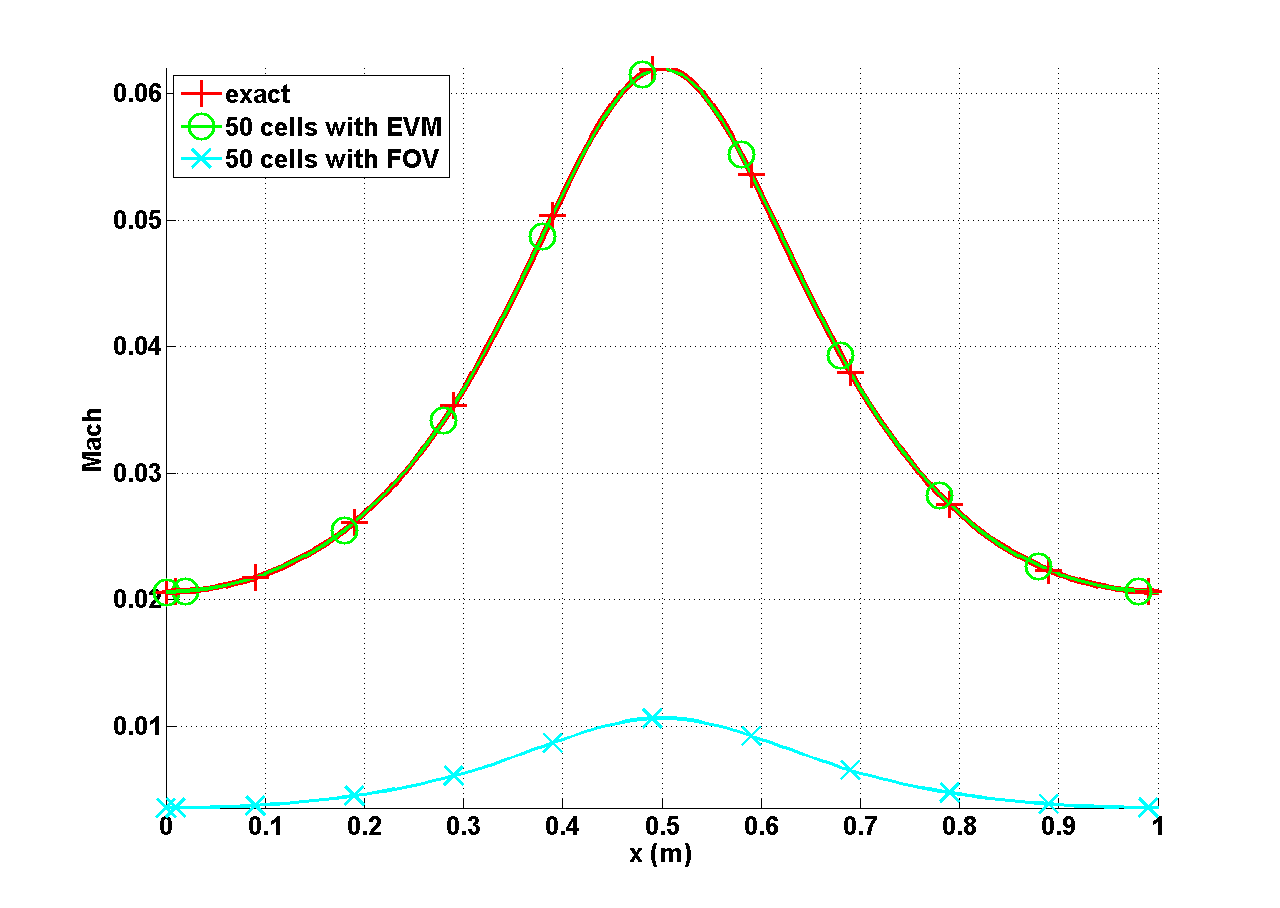
\includegraphics[width=\textwidth]{../figures/liquid_mach_numerical_and_exact_50.png}
                \caption{Mach number}
        \end{subfigure}%
        \begin{subfigure}[b]{0.37\textwidth}
                \centering
                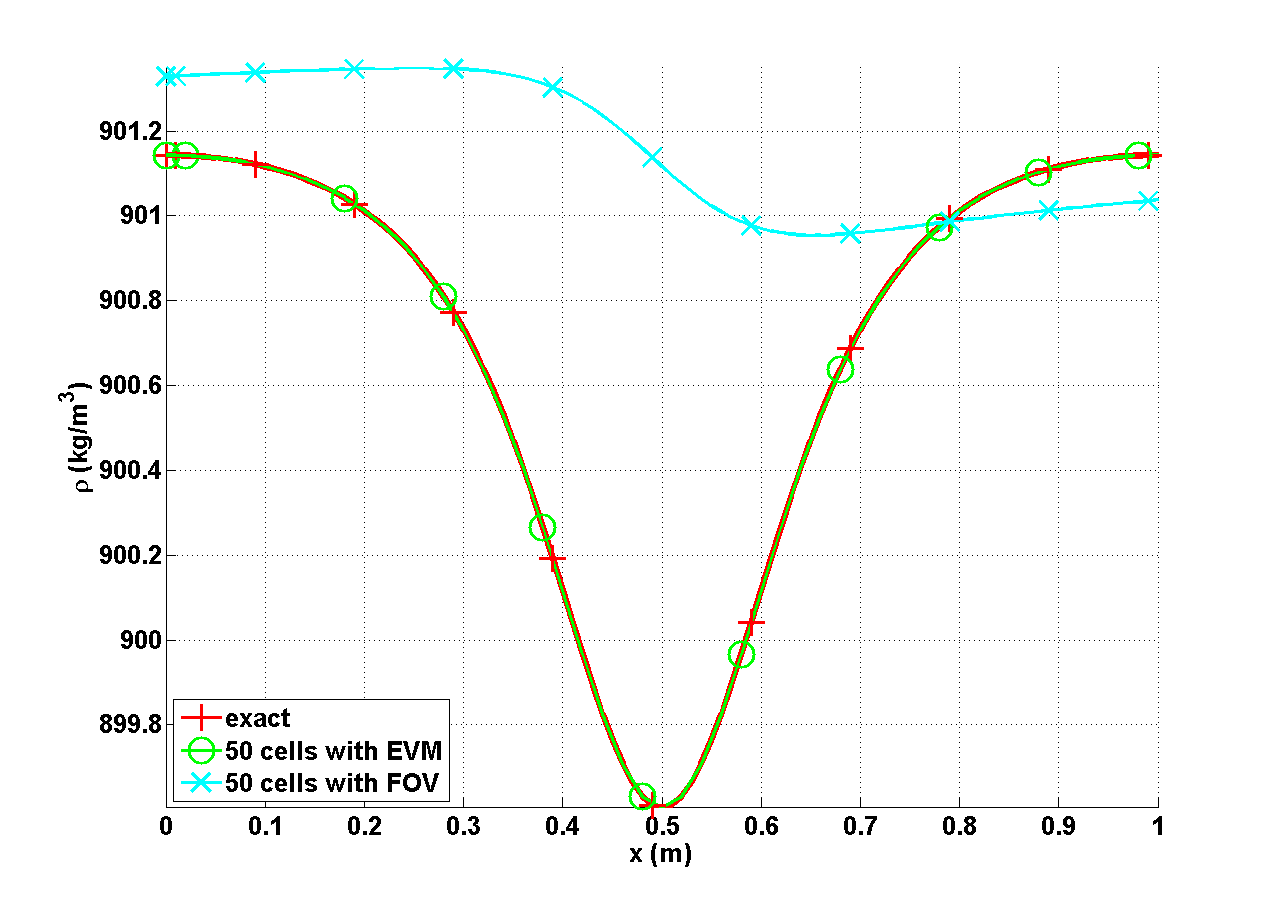
\includegraphics[width=\textwidth]{../figures/liquid_density_numerical_and_exact_50.png}
                \caption{Density}
        \end{subfigure}
        
        \begin{subfigure}[b]{0.37\textwidth}
                \centering
                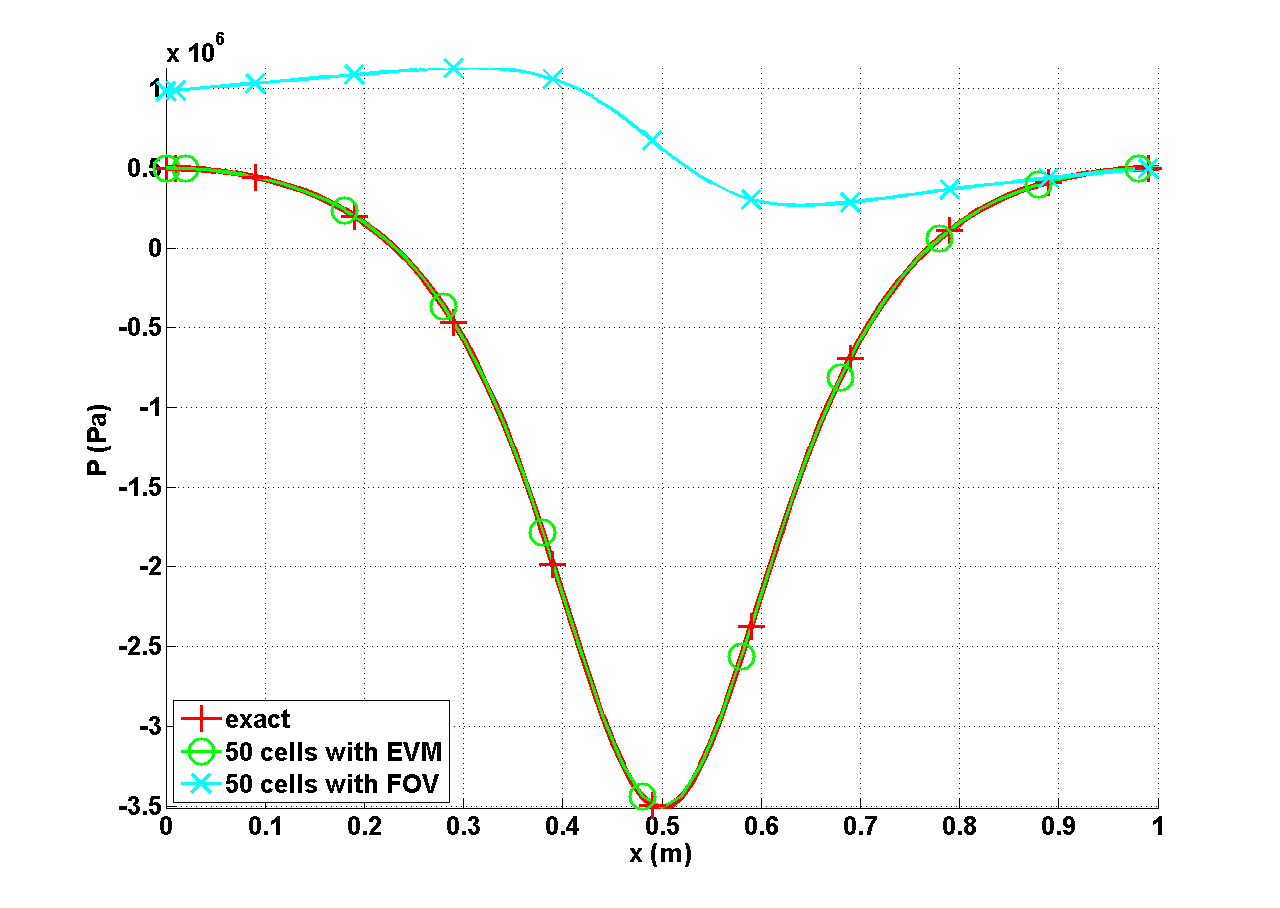
\includegraphics[width=\textwidth]{../figures/liquid_pressure_numerical_and_exact_50.png}
                \caption{Pressure}
        \end{subfigure}     
        \begin{subfigure}[b]{0.37\textwidth}
                \centering
                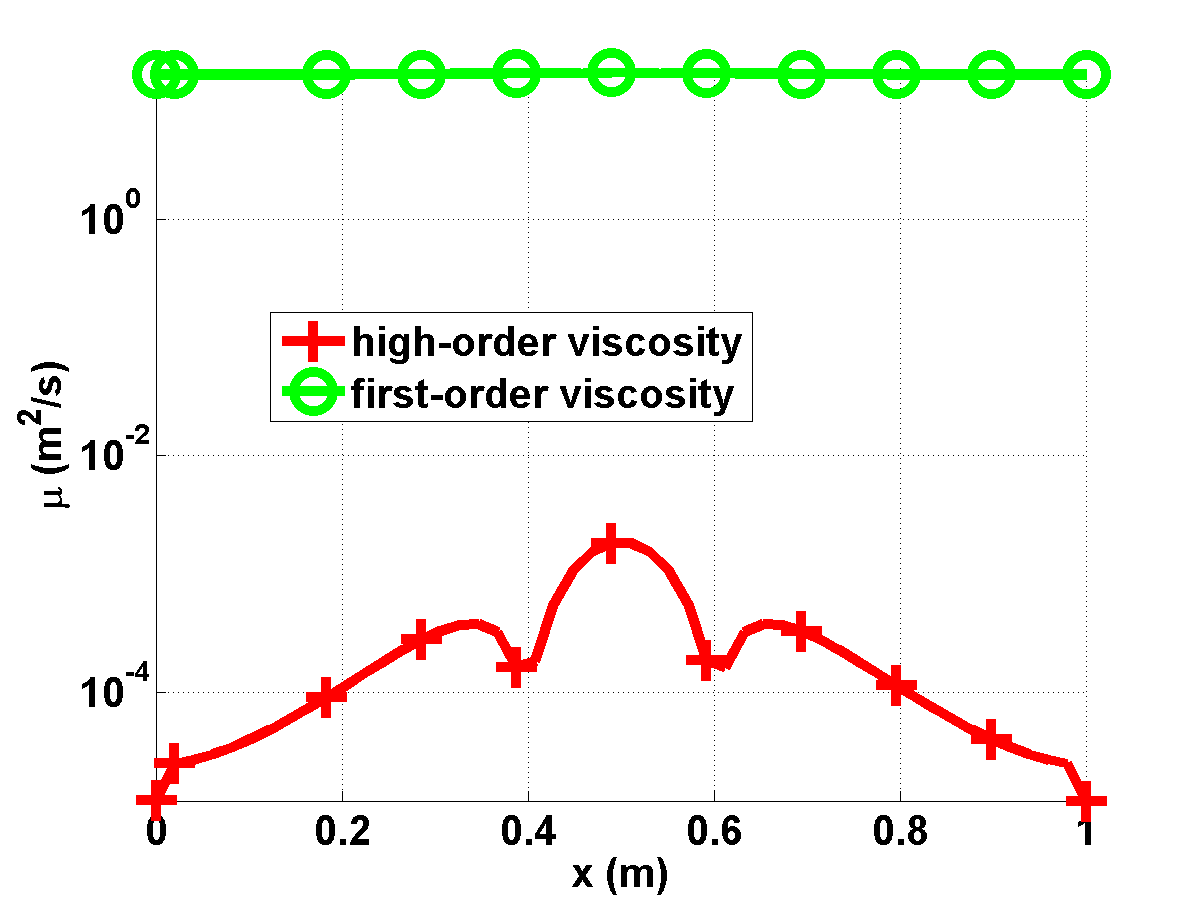
\includegraphics[width=\textwidth]{../figures/liquid_viscosity_numerical50.png}
                \caption{Viscosity coefficients}
        \end{subfigure}
\end{figure}
\end{frame}
%************************************************
\begin{frame}{$1$-D converging-diverging nozzle: liquid water}
\begin{center}
Convergence rates for the L$_1$ norm of the error:
\end{center}
\begin{table}[H]
\begin{center}
 \begin{tabular}{|c|c|c|c|c|c|c|c|c|}
 \hline
cells & density         & rate   & pressure        & rate    & velocity         & rate     \\ \hline
4    & 2.8037 $10^{-1}$ & $-$    & 8.4705 $10^{5}$ & $-$     & 7.2737           & $-$      \\ \hline
8    & 1.3343 $10^{-1}$ & 0.495 & 4.7893 $10^{5}$ & 0.24 & 6.1493           & 0.0747 \\ \hline
16   & 2.9373 $10^{-2}$ & 2.10 & 1.0613 $10^{5}$ & 2.09  & 1.2275           & 2.25   \\ \hline
32   & 5.1120 $10^{-3}$ & 2.58 & 1.8446 $10^{4}$ & 2.58  & 1.8943 $10^{-1}$ & 2.78   \\ \hline
64   & 1.0558 $10^{-3}$ & 2.31 & 3.7938 $10^{3}$ & 2.31  & 3.7919 $10^{-2}$ & 2.37   \\ \hline
128  & 2.3712 $10^{-4}$ & 2.18 & 8.4471 $10^{2}$ & 2.19  & 8.5517 $10^{-3}$ & 2.17   \\ \hline
256  & 5.6058 $10^{-5}$ & 2.08 & 1.9839 $10^{2}$ & 2.09  & 2.0475 $10^{-3}$ & 2.07   \\ \hline
512  & 1.3278 $10^{-5}$ & $2.07$ & 4.6622 $10^{1}$ & 2.08  & 4.9516 $10^{-4}$ & $2.06$   \\ \hline
1024  & 3.1193 $10^{-6}$ & $-$ & 1.1755 $10^{1}$ & $-$  & 1.2379 $10^{-4}$ & $-$   \\ \hline
\end{tabular}
\end{center}
\end{table}
\end{frame}
%************************************************
\begin{frame}{$1$-D converging-diverging nozzle: liquid water}
\begin{center}
Convergence rates for the L$_2$ norm of the error:
\end{center}
\begin{table}[H]
\begin{center}
 \begin{tabular}{|c|c|c|c|c|c|c|c|c|}
 \hline
cells& density            & rate & pressure          & rate & velocity           & rate \\ \hline
4    & 3.106397 $10^{-1}$ & $-$  & 5.254445 $10^{5}$ & $-$  & 3.288543           & $-$  \\ \hline
8    & 7.491623 $10^{-2}$ & 2.06 & 1.636966 $10^{5}$ & 1.62 & 1.823880           & 0.14 \\ \hline
16   & 2.079858 $10^{-2}$ & 1.81 & 4.627338 $10^{4}$ & 1.77 & 4.990605 $10^{-1}$ & 1.83 \\ \hline
32   & 5.329627 $10^{-3}$ & 1.96 & 1.180287 $10^{4}$ & 1.96 & 1.261018 $10^{-1}$ & 1.98 \\ \hline
64   & 1.341583 $10^{-3}$ & 1.99 & 2.967104 $10^{3}$ & 1.99 & 3.160914 $10^{-2}$ & 1.99 \\ \hline
128  & 3.359766 $10^{-4}$ & 1.99 & 7.428087 $10^{2}$ & 1.99 & 7.907499 $10^{-3}$ & 1.99 \\ \hline
256  & 8.403859 $10^{-5}$ & 1.99 & 1.857861 $10^{2}$ & 2.01 & 1.977292 $10^{-3}$ & 2.00 \\ \hline
512  & 2.10075  $10^{-5}$ & $-$ & 4.7024   $10^{1}$ & $-$ & 4.9516   $10^{-4}$ & $-$ \\ \hline
\end{tabular}
\end{center}
\end{table}
\end{frame}
%************************************************
\begin{frame}{$1$-D converging-diverging nozzle: vapor}
\begin{figure}[H]
        \centering
        \begin{subfigure}[b]{0.37\textwidth}
                \centering
                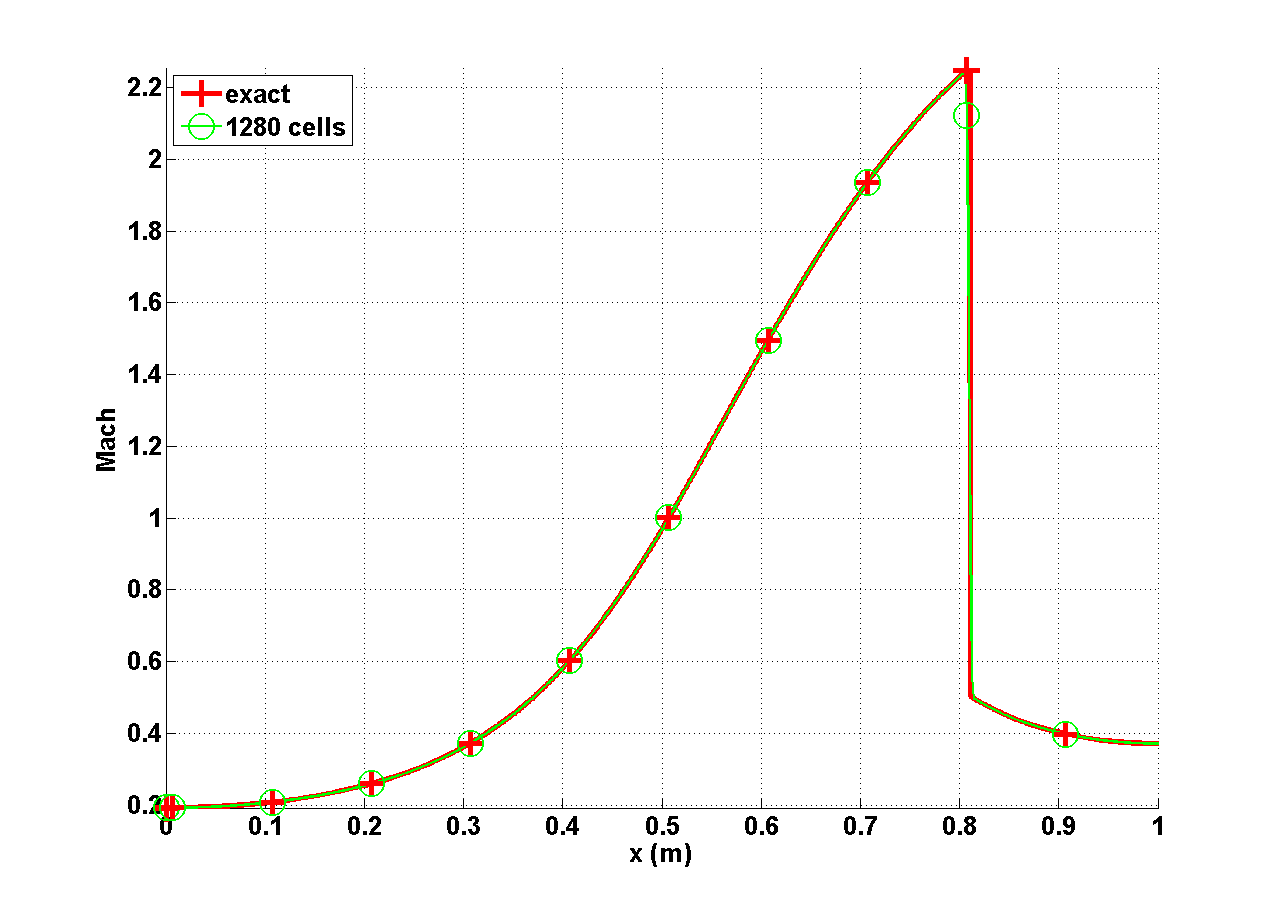
\includegraphics[width=\textwidth]{../figures/vapor_mach_numerical_and_exact_1280.png}
                \caption{Mach number}
        \end{subfigure}%
        \begin{subfigure}[b]{0.37\textwidth}
                \centering
                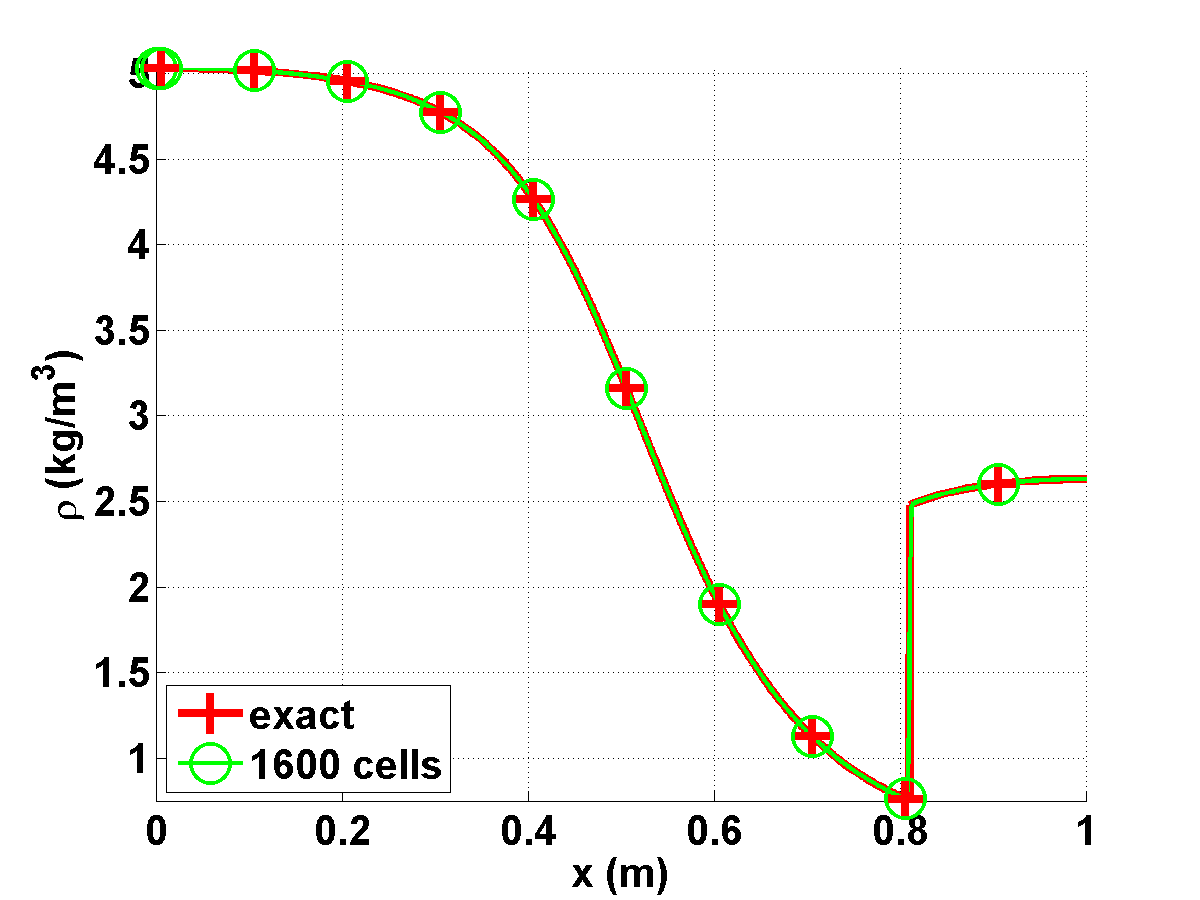
\includegraphics[width=\textwidth]{../figures/vapor_density_numerical_and_exact_1600.png}
                \caption{Density}
        \end{subfigure}

        \begin{subfigure}[b]{0.37\textwidth}
                \centering
                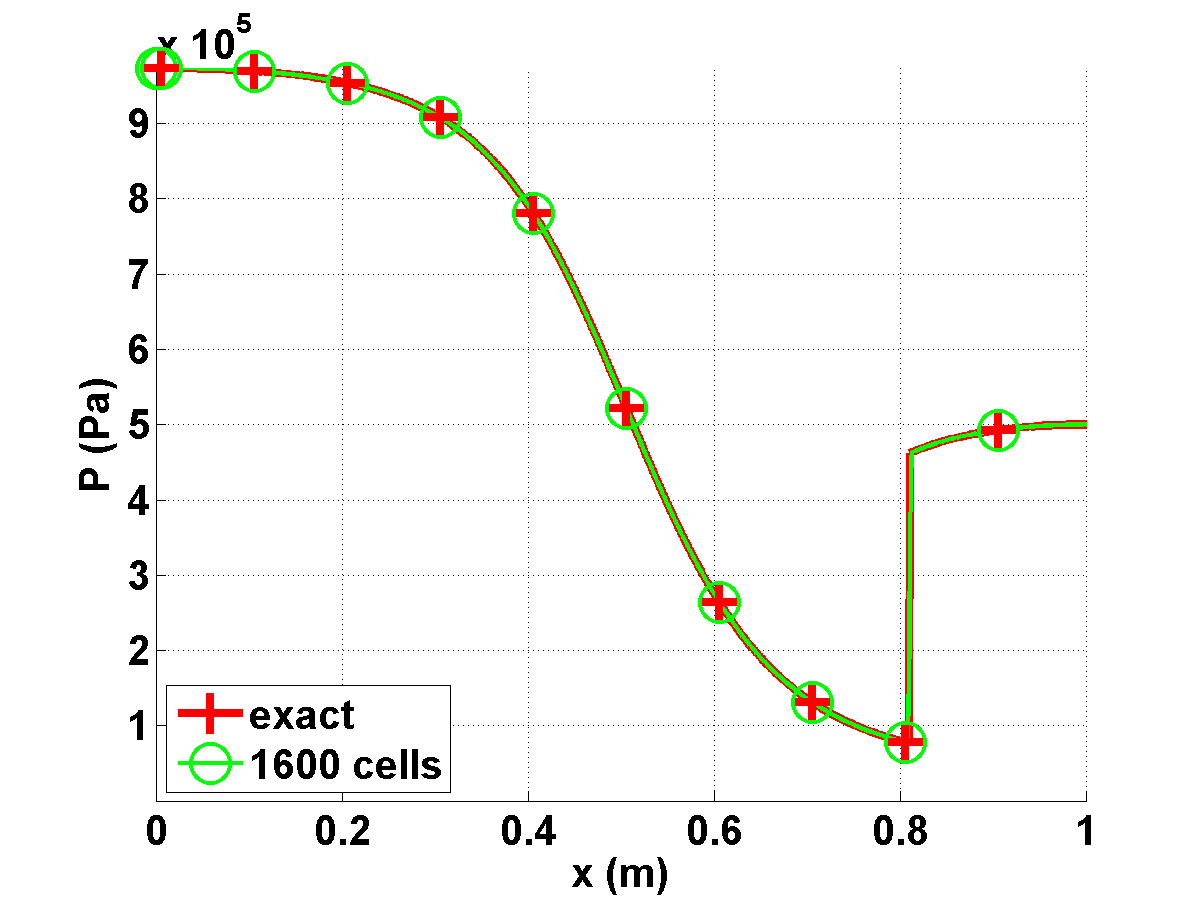
\includegraphics[width=\textwidth]{../figures/vapor_pressure_numerical_and_exact_1600.png}
                \caption{Pressure}
        \end{subfigure}
        \begin{subfigure}[b]{0.37\textwidth}
                \centering
                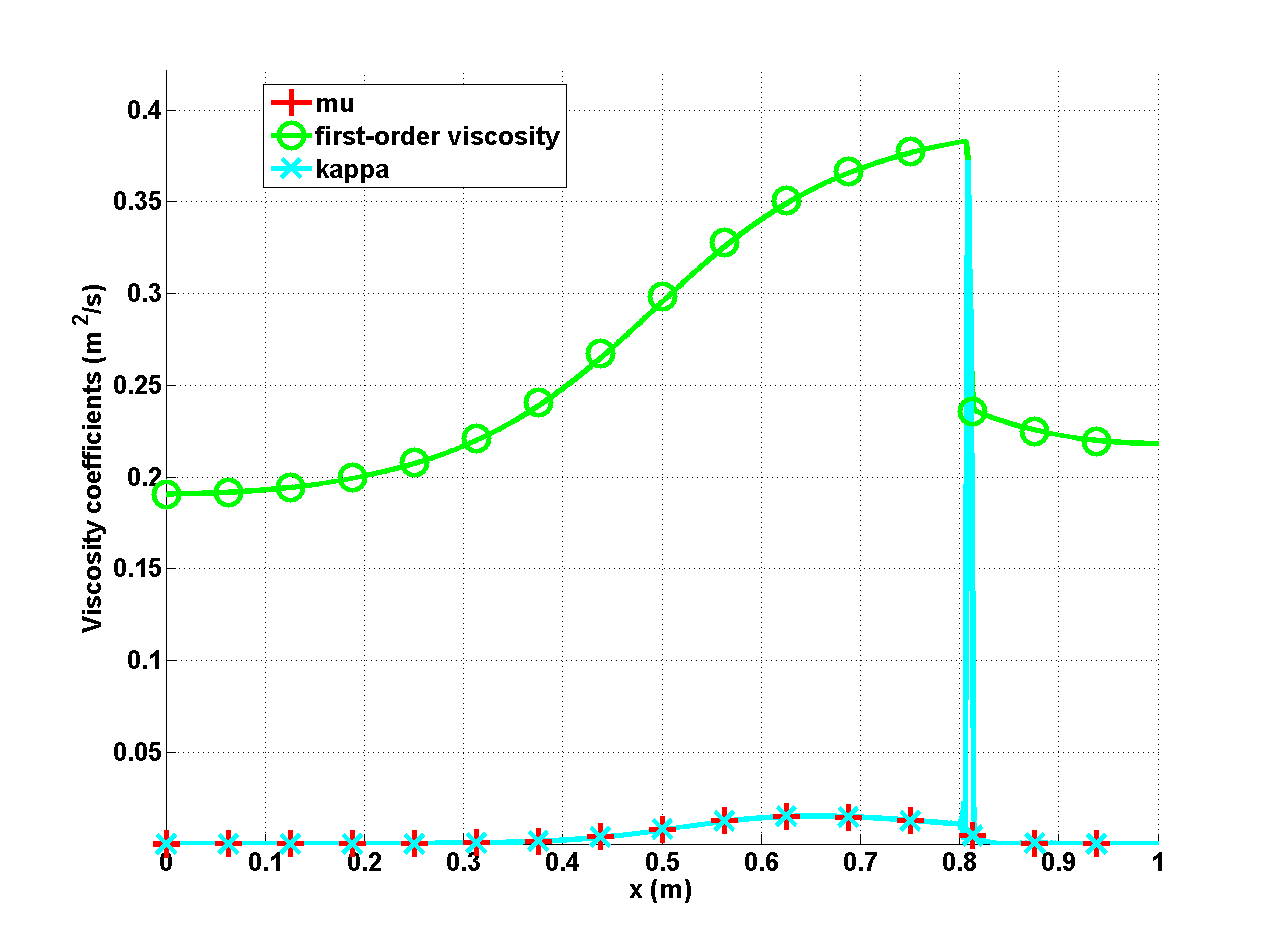
\includegraphics[width=\textwidth]{../figures/vapor_viscosity_numerical1600.png}
                \caption{Viscosity coefficients}
        \end{subfigure}
\end{figure}
\end{frame}
%************************************************
\begin{frame}{$1$-D converging-diverging nozzle: vapor}
\begin{center}
Convergence rates for the L$_1$ norm of the error:
\end{center}
\begin{table}[H]
\begin{center}
 \begin{tabular}{|c|c|c|c|c|c|c|c|c|}
 \hline
cells & density              & rate      & pressure          & rate      & velocity & rate      \\ \hline
$5$  & $0.72562$   $10^{-1}$ & $-$       & $1.5657$ $10^{5}$ & $-$       & $173.69$ & $-$       \\ \hline
$10$ & $0.4165$    $10^{-1}$ & $0.80088$ & $9.6741$ $10^{4}$ & $0.63425$ & $120.69$ & $0.52519$ \\ \hline
$20$ & $0.20675$   $10^{-1}$ & $1.0104$  & $4.9193$ $10^{4}$ & $0.96971$ & $72.149$ & $0.74228$ \\ \hline
$40$ & $0.093703$  $10^{-1}$ & $1.1417$  & $2.0103$ $10^{4}$ & $0.72728$ & $34.716$ & $1.0554$  \\ \hline
$80$ & $0.047328$  $10^{-1}$ & $0.9854$  & $1.0208$ $10^{4}$ & $0.9777$  & $16.082$ & $1.1101$  \\ \hline
$160$& $0.023965$  $10^{-2}$ & $0.9817$  & $5.1969$ $10^{3}$ & $0.9739$  & $7.9573$ & $1.0150$  \\ \hline
$320$& $0.020768$  $10^{-2}$ & $0.9886$  & $2.5116$ $10^{3}$ & $1.0490$  & $3.7812$ & $1.0734$  \\ \hline
$640$& $0.0059715$ $10^{-2}$ & $1.0160$  & $1.2754$ $10^{3}$ & $0.9776$  & $1.8353$ & $1.0428$  \\ \hline
\end{tabular}
\end{center}
\nonumber
\end{table}
\end{frame}
%************************************************
\begin{frame}{$1$-D converging-diverging nozzle: vapor}
\begin{center}
Convergence rates for the L$_2$ norm of the error:
\end{center}
\begin{table}[H]
\begin{center}
 \begin{tabular}{|c|c|c|c|c|c|c|c|c|}
 \hline
cells & density             & rate      & pressure          & rate      & velocity & rate       \\ \hline
$5$   & $9.7144$ $10^{-1}$  & $-$       & $2.0215$ $10^{5}$ & $-$       & $236.94$ & $-$        \\ \hline
$10$  & $5.9718$ $10^{-1}$  & $0.70195$ & $1.3024$ $10^{5}$ & $0.63425$ & $166.56$ & $0.50854$  \\ \hline
$20$  & $2.9503$ $10^{-1}$  & $1.0173$  & $6.6503$ $10^{4}$ & $0.96971$ & $103.36$ & $0.68831$  \\ \hline
$40$  & $1.8193$ $10^{-1}$  & $0.69747$ & $4.0171$ $10^{4}$ & $0.72728$ & $66.374$ & $0.6390$   \\ \hline
$80$  & $1.3366$ $10^{-1}$  & $0.44485$ & $2.3163$ $10^{4}$ & $0.43576$ & $42.981$ & $0.62692$  \\ \hline
$160$ & $9.6638$ $10^{-2}$  & $0.46790$ & $1.7263$ $10^{4}$ & $0.42413$ & $31.717$ & $0.43844$  \\ \hline
$320$ & $7.0896$ $10^{-2}$  & $0.44688$ & $1.2763$ $10^{4}$ & $0.43571$ & $23.138$ & $0.45499$  \\ \hline
$640$ & $5.2191$ $10^{-2}$  & $0.44190$ & $9.4217$ $10^{3}$ & $0.43790$ & $16.910$ & $0.45238$  \\ \hline
\end{tabular}
\end{center}
\nonumber
\end{table}
\end{frame}
%************************************************
\begin{frame}{$2$-D low-Mach flow over a cylinder}
\begin{block}{Typical benchmark problem for low-Mach flow:}
\begin{itemize}
\item The steady-state solution is symmetric: the iso-Mach contour lines are used to asses the symmetry of the numerical solution
\item The velocity at the top of the cylinder is twice the incoming velocity set at the inlet
\item The pressure fluctuations are proportional to the square of inlet Mach number, i.e., 
\begin{equation}
\delta P = \frac{\max(P(\vec{r},t)) - \min(P(\vec{r},t))}{\max(P(\vec{r},t))}  \propto M_\infty^2 \nonumber
\end{equation}
where $\delta P$ and $M_\infty$ denote the pressure fluctuations and the inlet Mach number, respectively.
\end{itemize}
\end{block}
\begin{block}{}
\begin{itemize}
\item triangular mesh with $4008$ triangular elements
\item Ideal Gas equation of state with $\gamma = 1.4$
\item CFL $= 20$
\end{itemize}
\end{block}
\end{frame}
%************************************************
\begin{frame}{$2$-D low-Mach flow over a cylinder}
\begin{figure}[H]
\centering
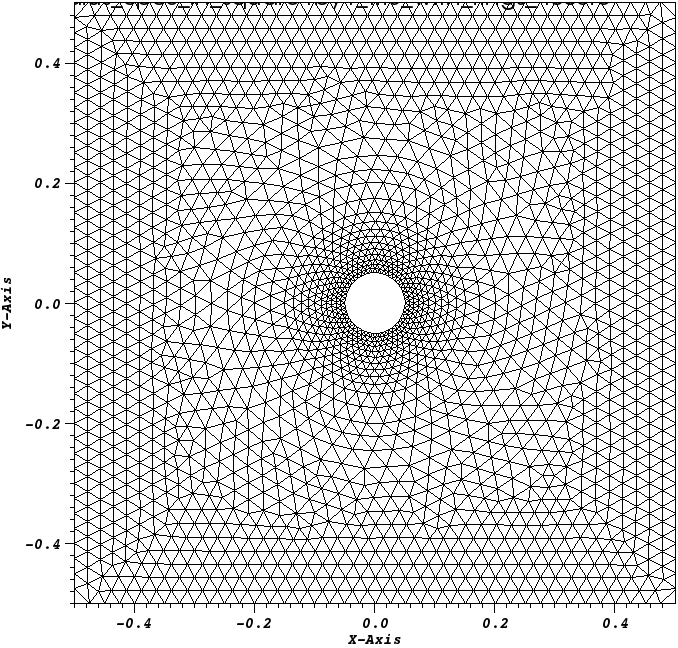
\includegraphics[width=0.6\textwidth]{../figures/Cylinder_geometry.png}
\end{figure}
\end{frame}
%************************************************
\begin{frame}{$2$-D low-Mach flow over a cylinder}
\begin{figure}
        \begin{subfigure}[b]{0.37\textwidth}
                \centering
                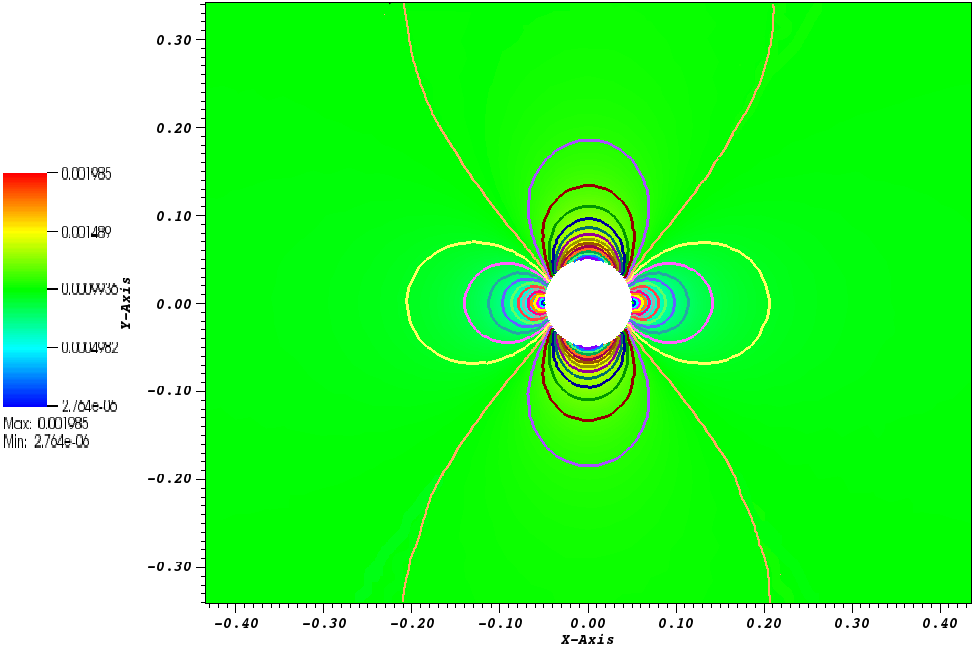
\includegraphics[width=\textwidth]{../figures/CylinderMach1em3ZoomIn.png}
                \caption{$M_{\text{inlet}}=10^{-3}$}
        \end{subfigure}%
        \begin{subfigure}[b]{0.37\textwidth}
                \centering
                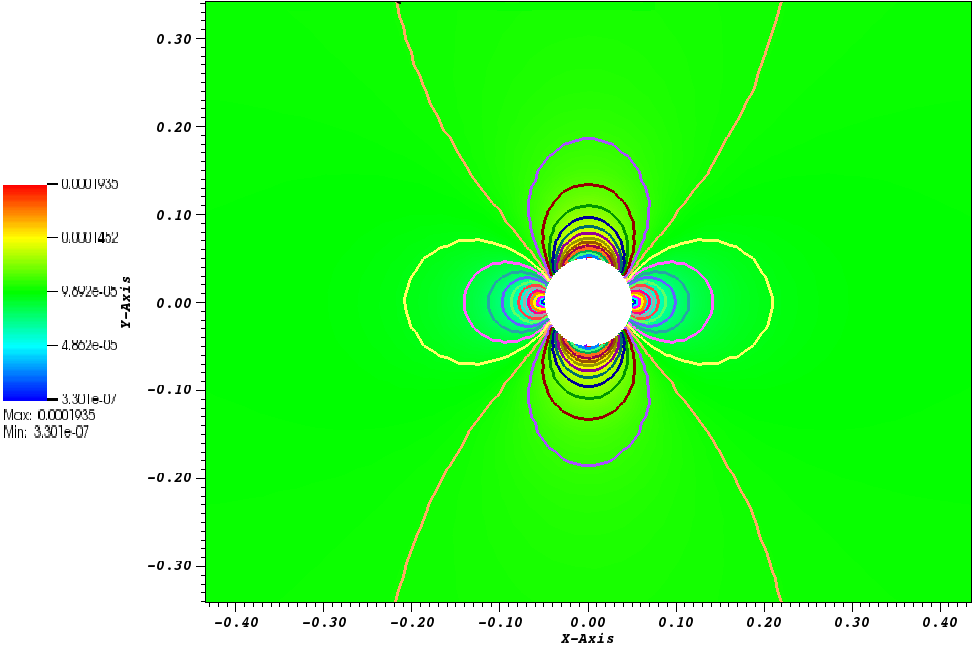
\includegraphics[width=\textwidth]{../figures/CylinderMach1em4ZoomIn.png}
                \caption{$M_{\text{inlet}}=10^{-4}$}
        \end{subfigure}    
  
        \begin{subfigure}[b]{0.37\textwidth}
                \centering
                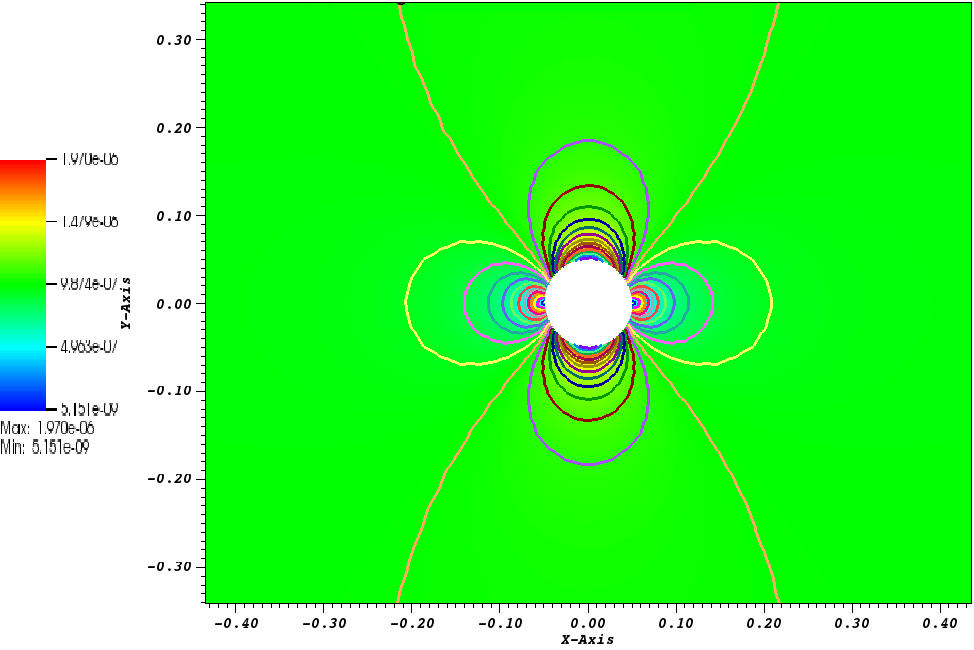
\includegraphics[width=\textwidth]{../figures/CylinderMach1em6ZoomIn.png}
                \caption{$M_{\text{inlet}}=10^{-6}$}
        \end{subfigure}%
        \begin{subfigure}[b]{0.37\textwidth}
                \centering
                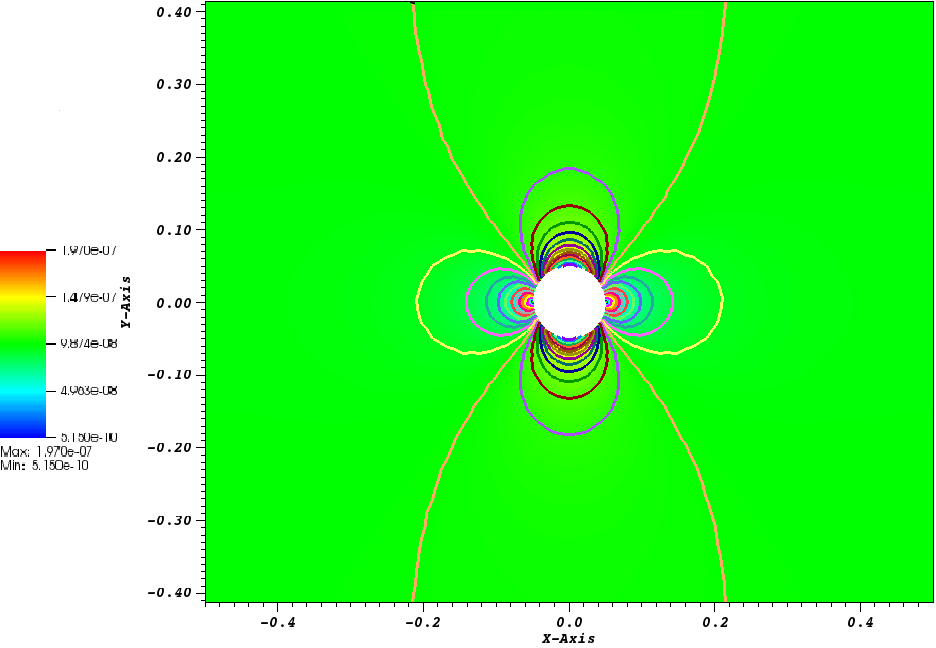
\includegraphics[width=\textwidth]{../figures/CylinderMach1em7ZoomIn.png}
                \caption{$M_{\text{inlet}}=10^{-7}$}
        \end{subfigure}    
\end{figure}        
\end{frame}
%************************************************
\begin{frame}{$2$-D low-Mach flow over a cylinder}
\begin{figure}[H]
\centering
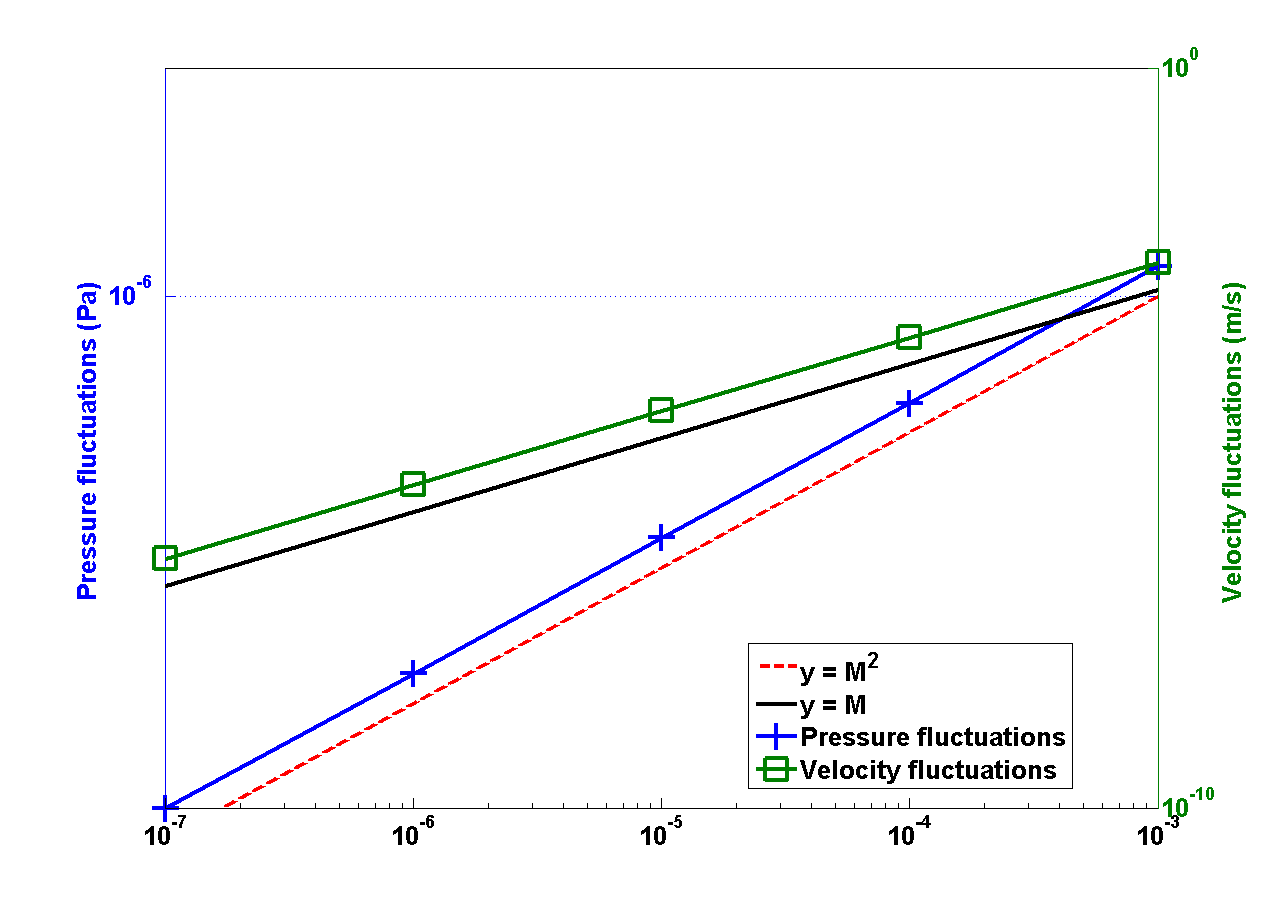
\includegraphics[width=\textwidth]{../figures/pressure_fluctuation.png}
\end{figure}
\end{frame}
%************************************************
\begin{frame}{$2$-D low-Mach flow over a cylinder}
\begin{center}
Velocity ratio for different Mach numbers
\end{center}
\begin{table}[H]
\begin{center}
\begin{tabular}{|c|c|c|c|}
\hline
Mach number & inlet velocity & velocity at the top of the cylinder & ratio \\ \hline
$10^{-3}$ & $2.348$ $10^{-3}$ & $1.176$ $10^{-3}$& $1.99$  \\ \hline
$10^{-4}$ & $2.285$ $10^{-4}$ & $1.145$ $10^{-4}$& $1.99$  \\ \hline
$10^{-5}$ & $2.283$ $10^{-5}$ & $1.144$ $10^{-5}$ & $1.99$ \\ \hline
$10^{-6}$ & $2.283$ $10^{-6}$ & $1.144$ $10^{-6}$ & $1.99$ \\ \hline
$10^{-7}$ & $2.283$ $10^{-7}$ & $1.144$ $10^{-7}$ & $1.99$ \\ \hline
\end{tabular}
\end{center}
\nonumber
\end{table}
\end{frame}
%************************************************
\begin{frame}{$2$-D low-Mach flow over a bump}
\begin{block}{Geometry: an uniform grid of $3352$ $Q_1$ elements}
\begin{figure}[H]
\centering
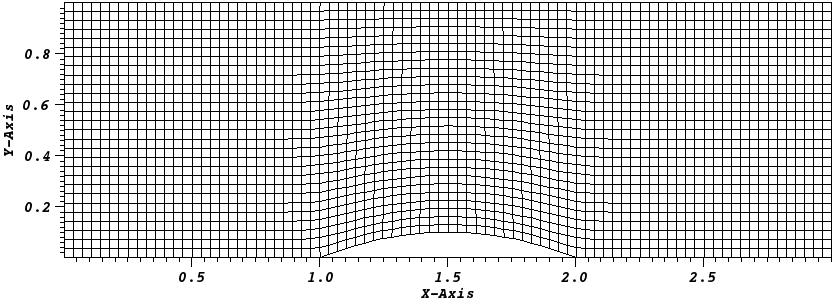
\includegraphics[width=\textwidth]{../figures/Hump2D_geometry.png}
\end{figure}    
\end{block}
\begin{block}{}
\begin{itemize}
\item Ideal Gas equation of state with $\gamma = 1.4$
\item CFL $= 20$
\item Inlet flow for different Mach numbers, static pressure and wall-boundary conditions.
\end{itemize}
\end{block}
\end{frame}
%************************************************
\begin{frame}{$2$-D low-Mach flow over a bump}
\begin{figure}
        \begin{subfigure}[b]{0.5\textwidth}
                \centering
                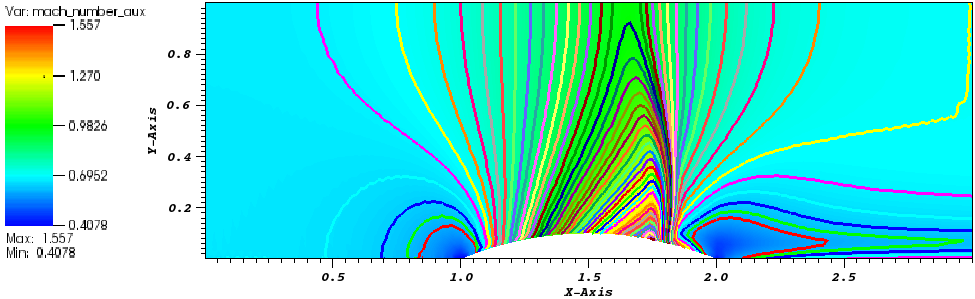
\includegraphics[width=\textwidth]{../figures/Hump2D_mach_0p7.png}
                \caption{$M_{\text{inlet}}=0.7$}
        \end{subfigure}%
        \begin{subfigure}[b]{0.5\textwidth}
                \centering
                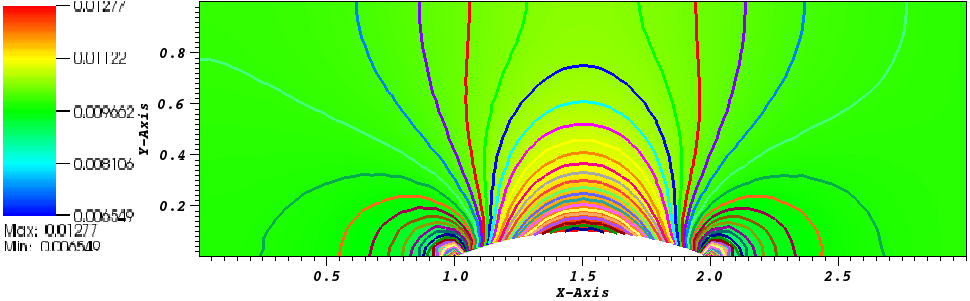
\includegraphics[width=\textwidth]{../figures/Hump2D_mach_0p01.png}
                \caption{$M_{\text{inlet}}=10^{-2}$}
        \end{subfigure}    
  
        \begin{subfigure}[b]{0.5\textwidth}
                \centering
                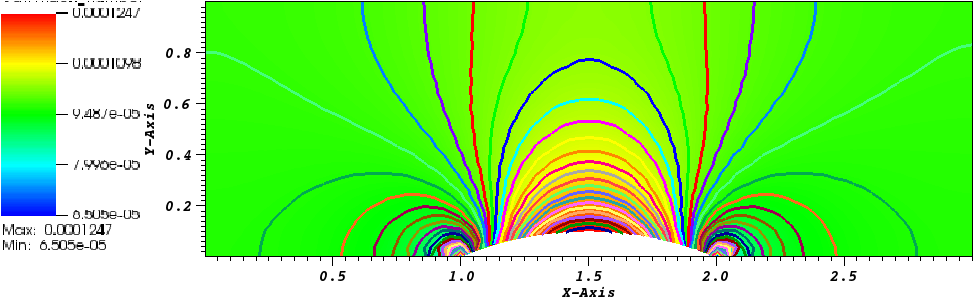
\includegraphics[width=\textwidth]{../figures/Hump2D_mach_1em4.png}
                \caption{$M_{\text{inlet}}=10^{-4}$}
        \end{subfigure}%
        \begin{subfigure}[b]{0.5\textwidth}
                \centering
                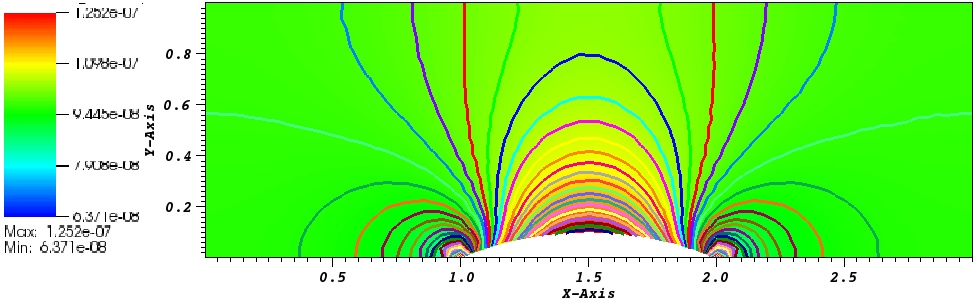
\includegraphics[width=\textwidth]{../figures/Hump2D_mach_1em7.png}
                \caption{$M_{\text{inlet}}=10^{-7}$}
        \end{subfigure}    
\end{figure}
\end{frame}
%************************************************
\begin{frame}{$2$-D Mach $2.5$ flow over a forward facing step}
  \begin{columns}
    \column{.5\textwidth}
       \includemedia[addresource=FFS_density_movie.mp4, activate=pageopen, deactivate=pageclose, width=6.5cm, height=5cm, flashvars={source=FFS_density_movie.mp4 & autoPlay=true & loop=true }]{}{VPlayer.swf}
    \column{.5\textwidth}
      \includemedia[addresource=FFS_viscosity_movie.mp4, activate=pageopen, deactivate=pageclose, width=6.5cm, height=5cm, flashvars={source=FFS_viscosity_movie.mp4 & autoPlay=true & loop=true }]{}{VPlayer.swf}
  \end{columns}
\end{frame}
%************************************************
\section{The multi-D seven-equation model with variable area}
\begin{frame}
\begin{center}
The SEVEN-EquAtion Model with variable area\\
(SEVEN-bandEd ArMadillo)
\end{center}
\begin{figure}[H]
\centering
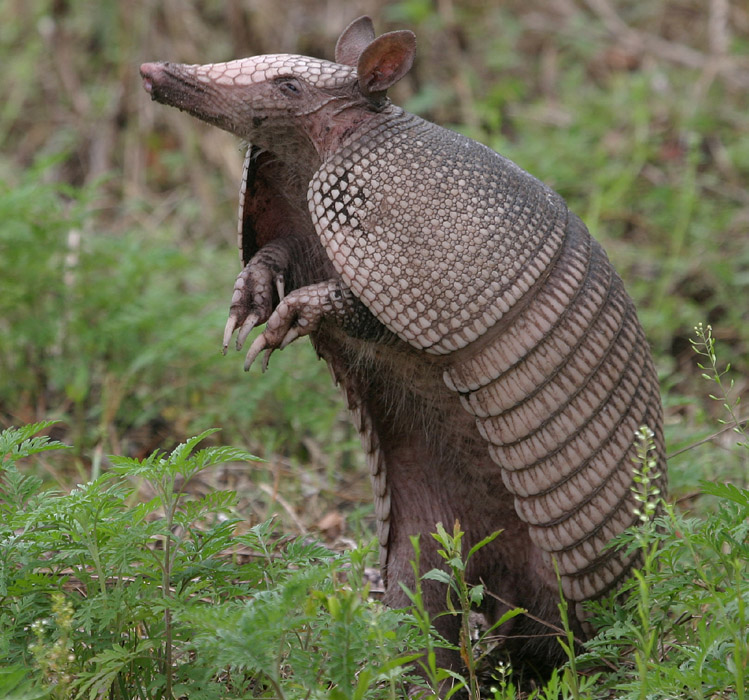
\includegraphics[width=0.5\textwidth]{../figures/seven_banded_armadillo.png}
\end{figure}   
\end{frame}
%************************************************
\begin{frame}{The seven-equation model (SEM)}
\begin{block}{The model}
\begin{itemize}
\setlength{\itemsep}{10pt}
\item Each phase obeys the single-phase Euler equations: two continuity equations, two momentum equations and two energy equations
\item Seventh equation: void fraction equation $\rightarrow$ an internal boundary condition between the two phases at the interface
\item Exchange terms between phases: relaxation terms. These terms were derived using \emph{rational thermodynamic} $\rightarrow$ consistent with the entropy minimum principle
\item {\color{red}The system of equations is well-posed and has seven waves}
\item The SEM degenerates to single-phase Euler equations when one phase disappears
\item The SEM degenerates into the 5-equation model of Kapila (2001) when using infinite relaxation coefficients
%\tcr{is there only one 5-eq model? should you add that is happens when relax param are set to be very large?}
\end{itemize}
\end{block}
\end{frame}
%************************************************
\begin{frame}{The seven-equation model (SEM)}
\begin{block}{Numerical stabilization methods}
\begin{itemize}
\setlength{\itemsep}{10pt}
\item discontinuous schemes (finite volume, DG)
\item approximate Riemann solvers: HLL, HLLC with low-Mach fix
\item apply upwind-type scheme for non-conservative flux
\end{itemize}
\end{block}
\begin{block}{Our approach}
\begin{itemize}
\setlength{\itemsep}{10pt}
\item continuous scheme
\item artificial dissipative method $\longrightarrow$ EVM
\end{itemize}
\end{block}
\end{frame}
%************************************************
\begin{frame}{The seven-equation model (SEM)}
We consider two phases ${j,k}$. Phase $k$ obeys the following system of equations:
\begin{align}
&\partial_t \left( \alpha_k  A\right) + \vec{u}_{int} A \grad \alpha_k = {\color{red}A \mu_P \left( P_k - P_j \right)} \nonumber
\end{align}
\begin{align}
&\partial_t \left( \alpha_k \rho_k A \right) + \div \left( \alpha_k \rho_k \vec{u}_k A \right) = 0 \nonumber
\end{align}
\begin{align}
\partial_t \left( \alpha_k \rho_k \vec{u}_k A \right) + \div \left[ \alpha_k A \left( \rho_k \vec{u}_k\otimes \vec{u}_k \right) \right]  + \grad(\alpha_k A P_k) &=  \nonumber \\
\alpha_k P_k \grad A &+  P_{int} A \grad \alpha_k +  {\color{red}A \lambda_u \left( \vec{u}_j - \vec{u}_k \right)} \nonumber
\end{align}
\begin{align}
\partial_t \left( \alpha_k \rho_k E_k A \right) + \div \left[ \alpha_k A \vec{u}_j \left( \rho_k E_k + P_k \right) \right] &= \nonumber\\
P_{int} \vec{u}_{int} A \grad \alpha_k - {\color{red}\mu_P \bar{P}_{int} \left( P_k-P_j \right)} &+{\color{red}\bar{\vec{u}}_{int} A \lambda_u \left( \vec{u}_j - \vec{u}_k \right)} \nonumber
\end{align}
\begin{equation}
\left\{
\begin{array}{l}
P_{int} = \bar{P}_{int} - \frac{\grad \alpha_k}{||\grad \alpha_k||} \frac{Z_k Z_j}{Z_k + Z_j} \cdot \left( \vec{u}_k-\vec{u}_j \right) \\
\bar{P}_{int} = \frac{Z_k P_j + Z_j P_k}{Z_k + Z_j} \\
\vec{u}_{int} = \bar{\vec{u}}_{int} - \frac{\grad \alpha_k}{||\grad \alpha_k||} \frac{P_k - P_j}{Z_k + Z_j} \\
\bar{\vec{u}}_{int} = \frac{Z_k \vec{u} _k + Z_j \vec{u}_j}{Z_k + Z_j} \\
\end{array}
\right.
\nonumber
\text{ and }
\left\{
\begin{array}{l}
\mu_P = \frac{A_{int}}{Z_k+Z_j} \\
\lambda_u = \frac{\mu_P}{2} Z_k Z_j \\
A_{int} = 6.25 \cdot A_{int,max} \alpha_k \left( 1-\alpha_k \right)^2
\end{array}
\right.
\end{equation}
%\tcr{$A_{int}$ expression is not symmetric. is this correct?}
\end{frame}
%************************************************
\begin{frame}{The seven-equation model (SEM)}
\begin{block}{Methodology}
\begin{enumerate}
\item derive the entropy equation WITHOUT the dissipative terms
\begin{align}
(s_e)_k^{-1} \alpha_k \rho_k A \frac{D s_k}{Dt} =& \textcolor{red}{\mu_P \frac{Z_k}{Z_k+Z_j} (P_j - P_k)^2} +
\textcolor{red}{ \lambda_u \frac{Z_j}{Z_k+Z_j} (\mbold u_j - \mbold u_k)^2} \nonumber \\ 
+& \textcolor{red}{|| \grad \alpha_k || \frac{Z_k }{\left( Z_k+Z_j \right)^2} \left[ Z_j (\vec{u}_j-\vec{u}_k)\right.+\left. \frac{\grad \alpha_k}{|| \grad \alpha_k ||}(P_k-P_j)\right]^2 }\nonumber
\end{align}
\item same steps as for the multi-D Euler equations: recast the entropy residual, viscous regularization, non-dimensionalized equations, viscosity coefficients.
\end{enumerate}
\end{block}
\begin{block}{A particularity}
Two phases $\to$ two entropy residuals $\to$ two options to derive the dissipative terms: \\
(a) either we consider the total entropy residual by summing over the phases \\
(b) or, we consider each phase independently of each other which will automatically ensure positivity of the total entropy \\
\end{block}
\end{frame}
%************************************************
\begin{frame}{Viscous regularization for the multi-D SEM:}
\begin{block}{}
\begin{align}
&\partial_t \left( \alpha_k  A\right) + \vec{u}_{int} A \grad \alpha_k = {\color{red}A \mu_P \left( P_k - P_j \right)} + {\color{blue}\div \vec{l}_k} \nonumber \\
\vspace{6pt}
&\partial_t \left( \alpha_k \rho_k A \right) + \div \left( \alpha_k \rho_k \vec{u}_k A \right) = {\color{blue}\div \vec{f}_k} \nonumber
\end{align}
\begin{align}
\partial_t \left( \alpha_k \rho_k \vec{u}_k A \right) + \div \left[ \alpha_k A \left( \rho_k \vec{u}_k\otimes \vec{u}_k + P_k\mathbb{I}\right) \right] &=  \nonumber \\
\alpha_k P_k \grad A +  P_{int} A \grad \alpha_k &+  {\color{red}A \lambda_u \left( \vec{u}_j - \vec{u}_k \right)} +{\color{blue}\div \bar{g}_k}\nonumber
\end{align}
\begin{align}
\partial_t \left( \alpha_k \rho_k E_k A \right) + \div \left[ \alpha_k A \vec{u}_j \left( \rho_k E_k + P_k \right) \right] &= \nonumber \\
P_{int} \vec{u}_{int} A \grad \alpha_k - {\color{red}\mu_P \bar{P}_{int} \left( P_k-P_j \right)} &+{\color{red}\bar{\vec{u}}_{int} A \lambda_u \left( \vec{u}_j - \vec{u}_k \right)} + {\color{blue}\div \vec{h}_k} \nonumber
\end{align}
\end{block}
\begin{block}{}
\begin{equation}
\left\{
\begin{array}{lcl}
{\color{blue}\vec{l}_k} = ? \\ %A {\color{magenta}\beta_k} \grad \alpha_k & & \\
{\color{blue}\vec{f}_k} = \alpha_k A {\color{magenta}\kappa_k}  \grad \rho_k + \rho_k \vec{l}_k& & \\
{\color{blue}\bar{g}_k} = \alpha_k A \rho_k {\color{magenta}\mu_k} \grad^s \vec{u}_k + \vec{u}_k \otimes \vec{f}_k & & \\
{\color{blue}\vec{h}_k} = \alpha_k A {\color{magenta}\kappa_k} \grad(\rho_k e_k) - \frac{||\vec{u}_k||^2}{2} \vec{f}_k + \vec{u} \cdot \bar{g}_k + \rho_k e_k \vec{l}_k & &
\end{array}
\right.
\nonumber
\end{equation}
\end{block}
%Entropy equation:
%\begin{eqnarray}
%\alpha_k A \rho_k \frac{ds_k}{dt} + \left( {\color{green}\alpha_k A \kappa_k  \grad \rho_k} + {\color{red}\rho_k l_k} \right) \grad s_k - {\color{green}\div \left( \alpha_k A \rho_k \grad s_k \right)} = \nonumber \\ {\color{green}\partial_e s_k \alpha_k A \rho_k \mu_k \grad^s \vec{u} :  \grad \vec{u}}- {\color{green}X_k \Sigma_k X_k^t} + {\color{blue}Q}
%\nonumber
%\end{eqnarray}
\end{frame}
%************************************************
\begin{frame}{How to derive the dissipative term $\vec{l}$ ?}
\begin{equation}
\partial_t \left( \alpha_k  A\right) + A \vec{u}_{int} \cdot \grad \alpha_k = {\color{blue}\div \vec{l}_k} \nonumber
\end{equation}
\begin{block}{}
\begin{itemize}
\item scalar hyperbolic equation with eigenvalue $\vec{u}_{int}$
\item by analogy to the Burger's equation $\to$ $\vec{l}_k = A \beta_k \grad \alpha_k$
\item this regularization ensures positivity of $\alpha_k$
\item $\beta_k$ is a positive viscosity coefficient:
\begin{align}
&\beta_k = \max ( \beta_{k,e}, \beta_{max}) \text{ where }\nonumber \\
&\beta_{max} = \frac{h}{2} || \vec{u}_{int} || \text{ and } \beta_{k,e} = h^2 \frac{\max( R_\alpha, J_\alpha )}{|| \eta - \bar{\eta} ||_\infty} \nonumber \\
&R_\alpha = \partial_t \eta + \vec{u}_{int}\cdot \grad \eta \text{ with } \eta = \frac{\alpha_k^2}{2}  \nonumber
\end{align}
\end{itemize}
\end{block}
$\rightarrow$ when assuming $\mu_k = \kappa_k = \beta_k$, the parabolic regularization is retrieved
\end{frame}
%************************************************
\begin{frame}{What about the viscosity coefficients $\mu_k$ and $\kappa_k$?}
\begin{subequations}
%
\begin{equation}
\mu_k(\vec{r},t)    = \min \Big (\mu_{\max ,k}(\vec{r},t), \mu_{e,k} (\vec{r},t)    \Big) \text{  and  }
\kappa_k(\vec{r},t) = \min \Big (\mu_{\max ,k}(\vec{r},t), \kappa_{e,k} (\vec{r},t) \Big ) \nonumber
\end{equation}
%
where the first-order viscosity is given by
\begin{equation}
  \kappa_{\max ,k}(\vec{r},t)  = \mu_{\max ,k} (\vec{r},t) = \frac{h}{2} \Big ( ||\vec{u}_k|| + c_k \Big ) \nonumber
\end{equation}
%
and the entropy viscosity coefficients by 
%
\begin{equation}
\kappa_{e,k}(\vec{r},t) = \frac{h^2 \max(\resinew_k, J_k)}{ \rho_k c_k^2 }  \text{  and  }
\mu_{e,k}(\vec{r},t)    = \frac{h^2 \max(\resinew_k, J_k)}{ \norm_{P,k}^\mu} \nonumber
\end{equation}
%
where
%
\begin{equation}
\norm_{P,k}^\mu =  \left\{
\begin{array}{ll}
 \rho_k ||\vec{u}_k ||^2       & \text{ if } \left| \resinew_k^* \right| \geq M_k \text{ (i.e., non-isentropic flow)} \\
 \rho_k c_k^2 = \norm_{P,k}^\kappa & \text{ otherwise} 
\end{array}
\right. \nonumber
\end{equation}
% 
with the jumps given by
%
\begin{equation}
J_k = || \vec{u}_k || \max \Big ( [[ \grad P_k \cdot \vec{n} ]], c_k^2 [[\grad \rho_k \cdot \vec{n}]] \Big) \nonumber
\end{equation}
\end{subequations}
\end{frame}
%************************************************
\begin{frame}{Numerical results}
\begin{block}{$1$-D shock tube}
\begin{itemize}
\setlength{\itemsep}{10pt}
\item two independent fluids
\item two fluids with pressure and velocity relaxation terms
\end{itemize}
\end{block}
\end{frame}
%************************************************
\begin{frame}{$1$-D shock tube with two independent fluids}
\begin{block}{}
\begin{itemize}
\setlength{\itemsep}{5pt}
\item two fluids (1 and 2) described with ideal gas equation of state: $P = (\gamma-1) \rho e$
\item heavy fluid with $\gamma_1=3$ and light fluid with $\gamma_2 =1.4$
\item no interaction between the two fluids ($\mu_P=\lambda_u=0$) $\longrightarrow$ same as running a single-phase flow code twice
\item exact solution is available and obtained from a Riemann solver
\item $500$ cells, CFL$=1$ and $t_{flinal} = 305 \mu s$ 
\item initial step pressure: $P_{left} = 1 MPa$ and $P_{right} = 0.1 MPa$
\item fluids are initially at rest and uniform volume fraction $\alpha_i = 0.5$
\item uniform initial density $\rho_1 = 10 kg \cdot m^{-3}$ and $\rho_2 = 1 kg \cdot m^{-3}$
\end{itemize}
\end{block}
Objective: verify that the dissipative terms does not affect the volume fraction profile
\end{frame}
%************************************************
\begin{frame}{$1$-D shock tube with two independent fluids}
\begin{figure}
        \begin{subfigure}[b]{0.37\textwidth}
                \centering
                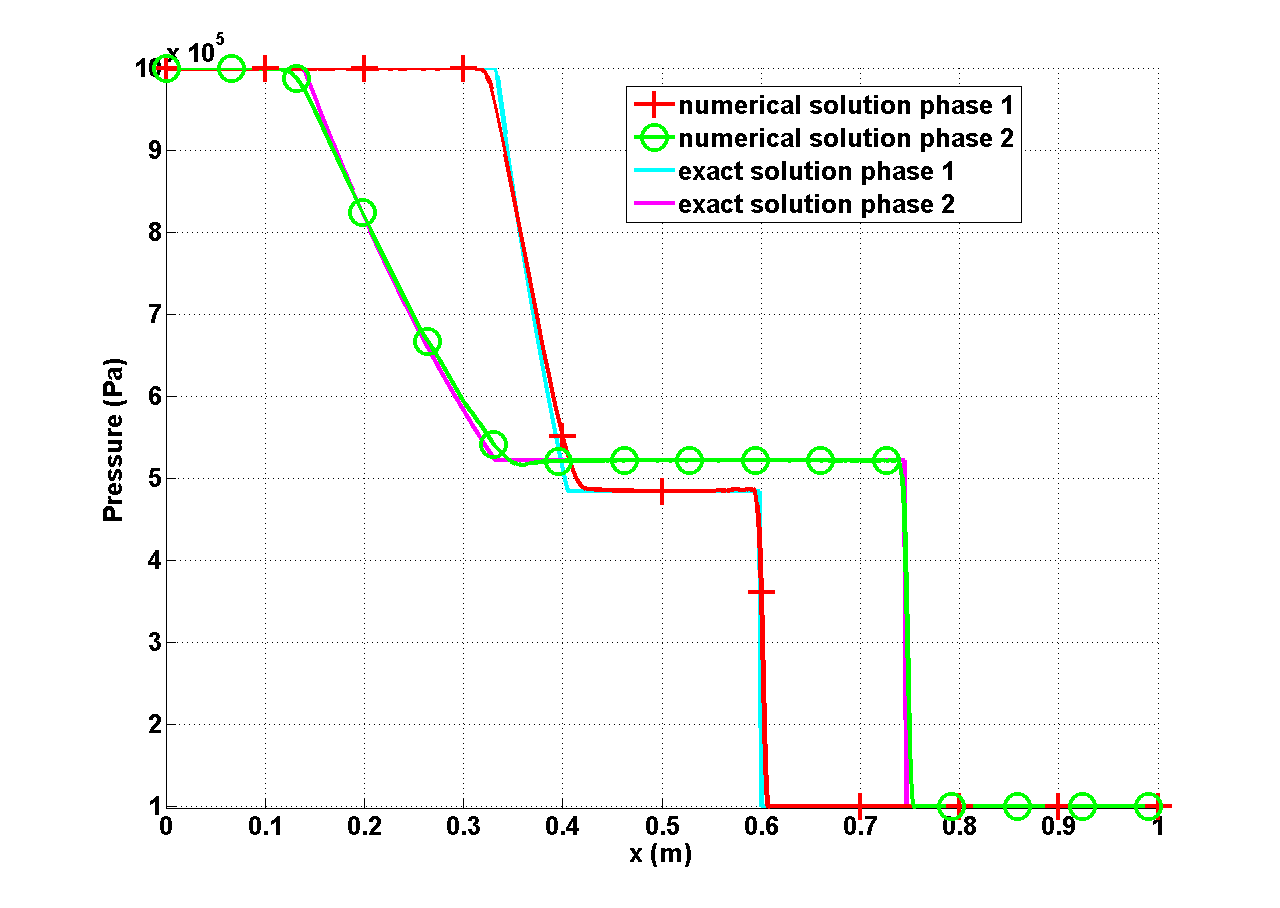
\includegraphics[width=\textwidth]{../figures/SEM/two_phases_pressure.png}
                \caption{Pressure at $t=305$ $\mu s$}
        \end{subfigure}%
        \begin{subfigure}[b]{0.37\textwidth}
                \centering
                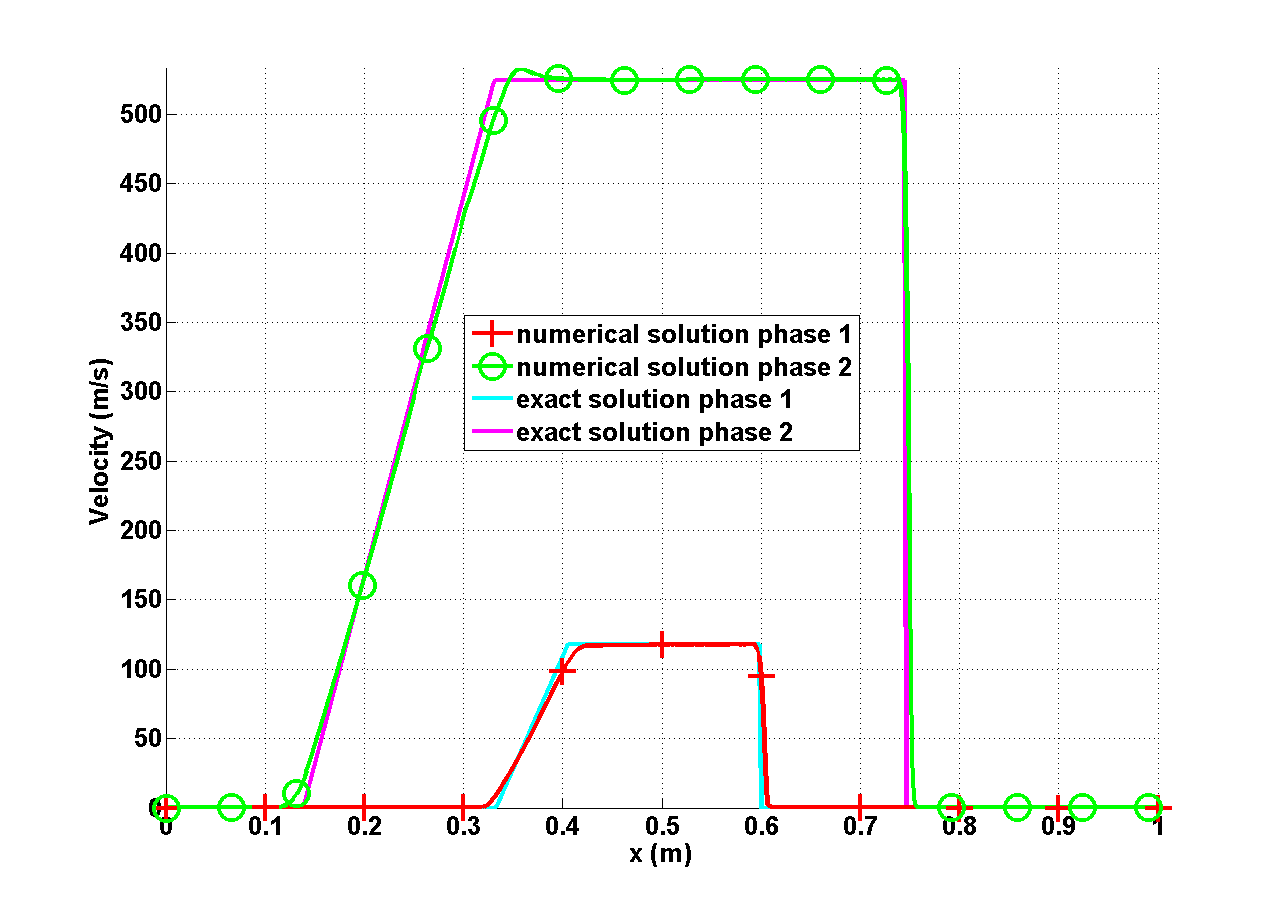
\includegraphics[width=\textwidth]{../figures/SEM/two_phases_velocity.png}
                \caption{Velocity at $t=305$ $\mu s$}
        \end{subfigure}%

        \begin{subfigure}[b]{0.37\textwidth}
                \centering
                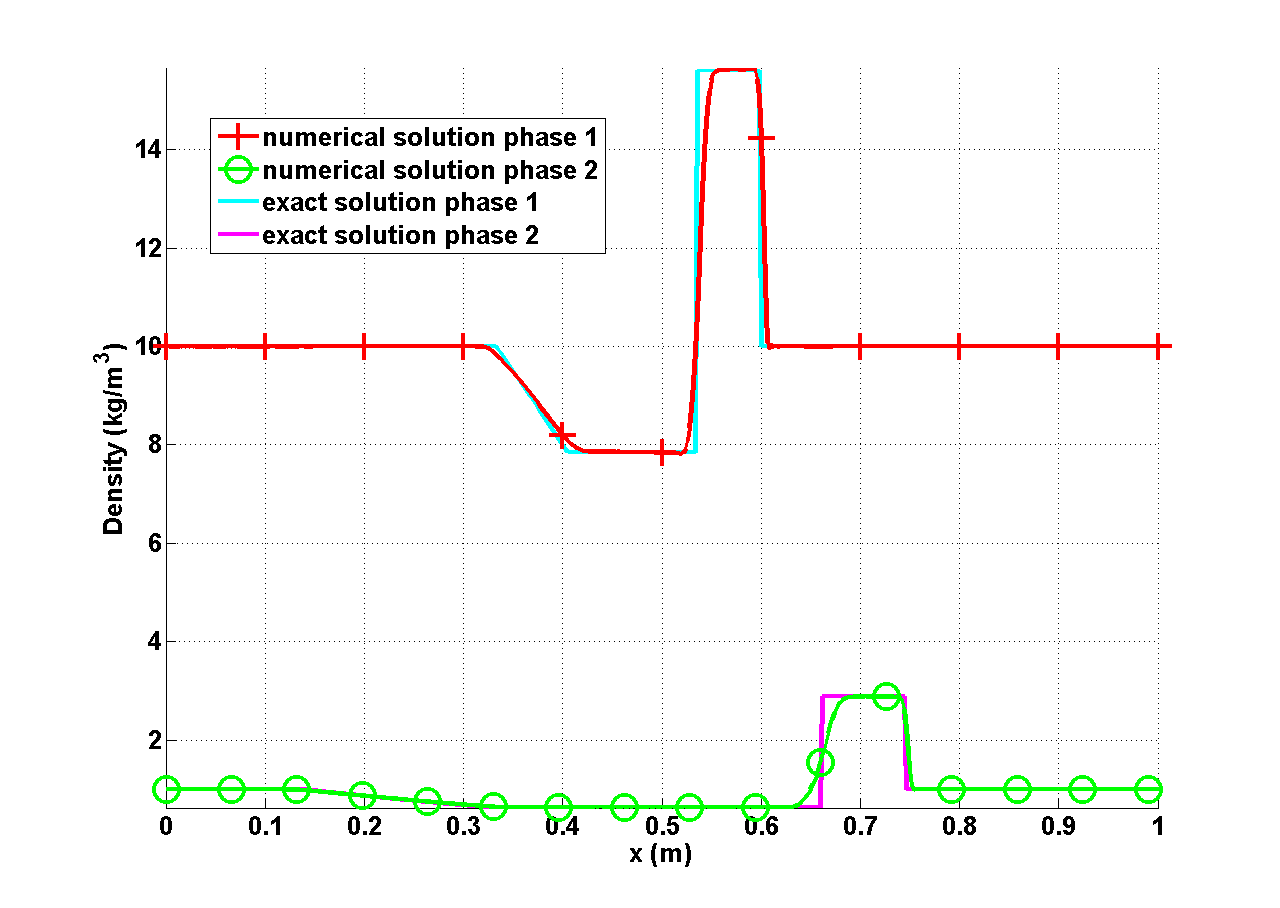
\includegraphics[width=\textwidth]{../figures/SEM/two_phases_density.png}
                \caption{Pressure at $t=305$ $\mu s$}
        \end{subfigure}%
        \begin{subfigure}[b]{0.37\textwidth}
                \centering
                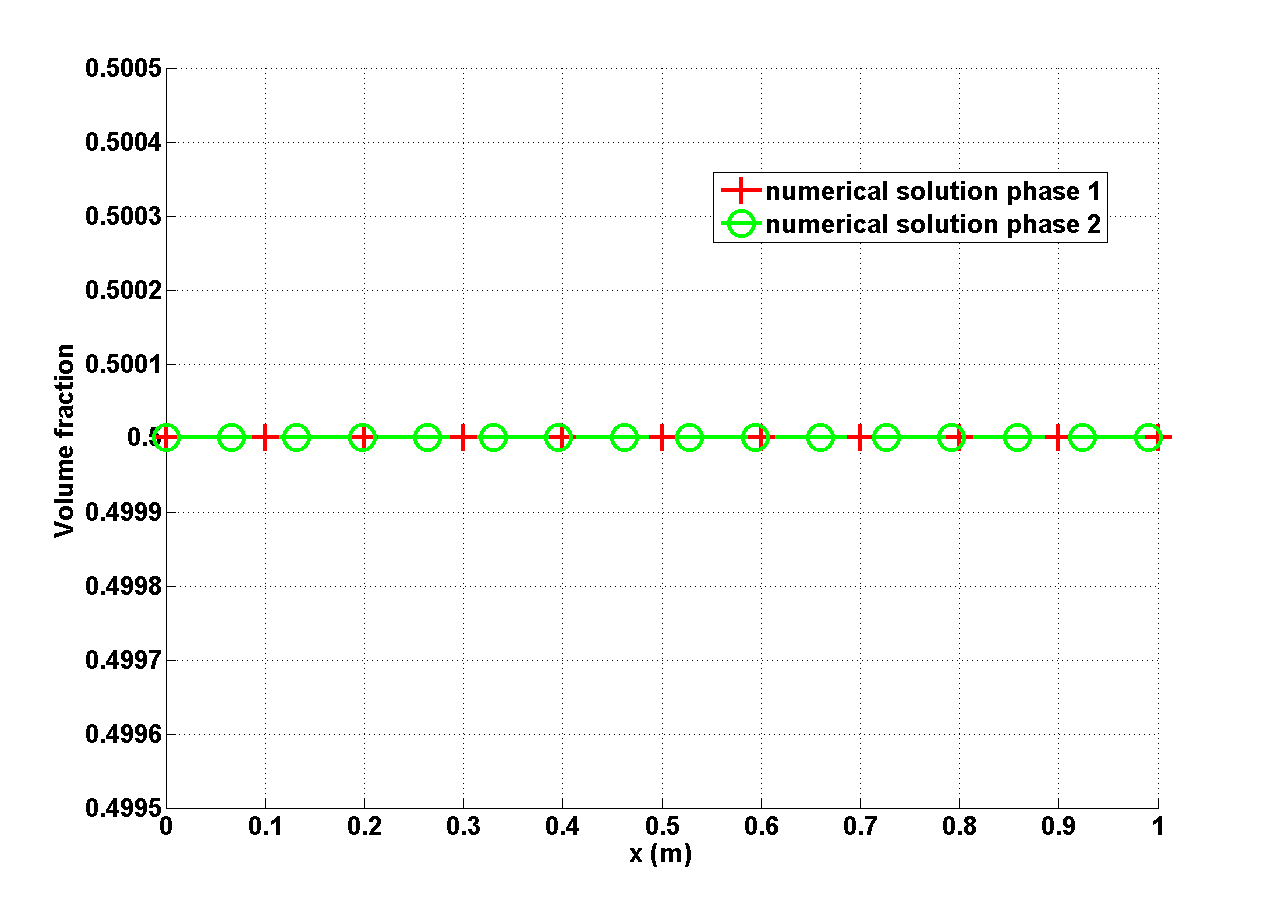
\includegraphics[width=\textwidth]{../figures/SEM/two_phases_volume_fraction.png}
                \caption{Velocity at $t=305$ $\mu s$}
        \end{subfigure}%
\end{figure}
\end{frame}
%************************************************
\begin{frame}{$1$-D shock tube with two independent fluids}
\begin{figure}
        \begin{subfigure}[b]{0.37\textwidth}
                \centering
                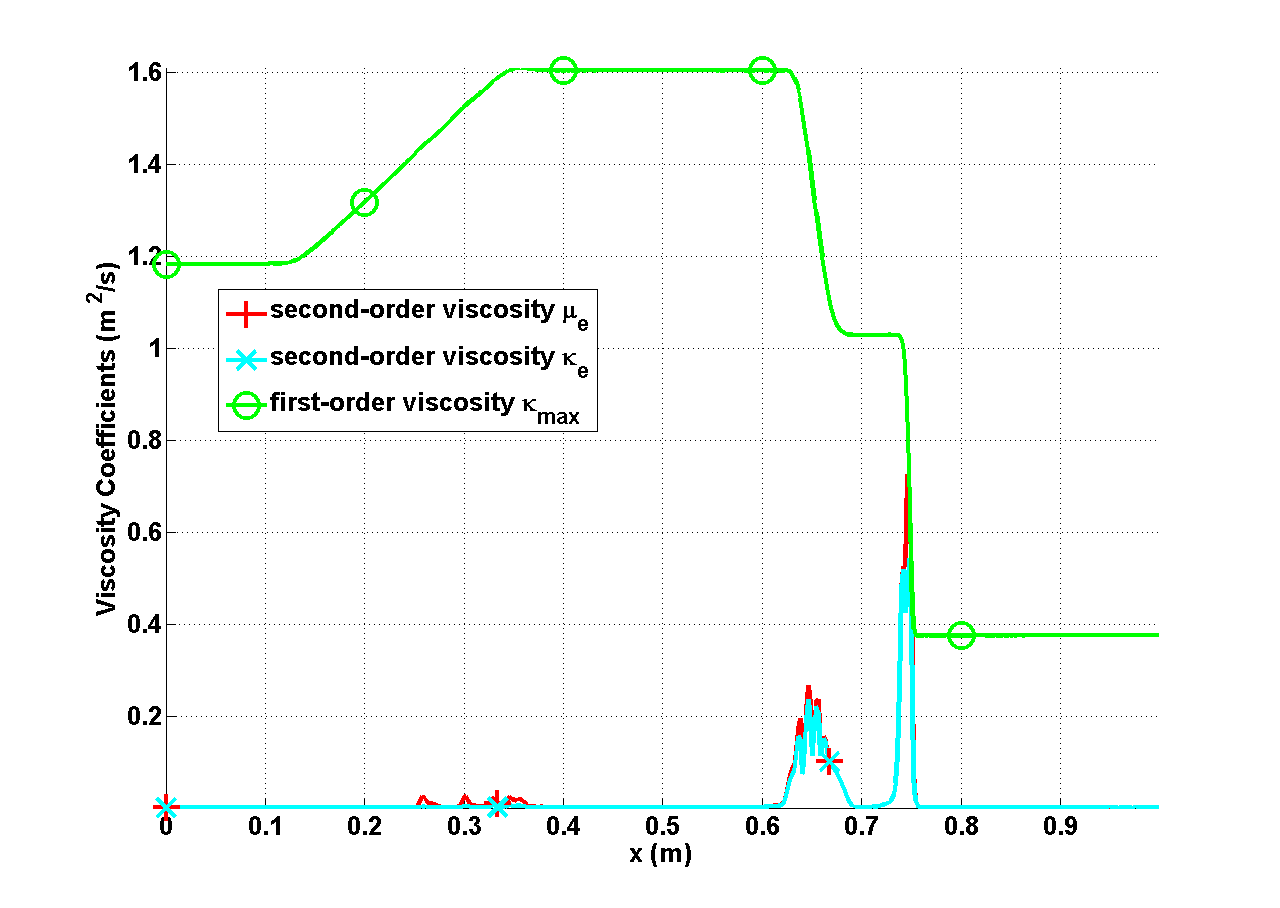
\includegraphics[width=\textwidth]{../figures/SEM/two_phases_liquid_viscosity_kappa_mu.png}
                \caption{Viscosity coefficients phase $1$}
        \end{subfigure}%
        \begin{subfigure}[b]{0.37\textwidth}
                \centering
                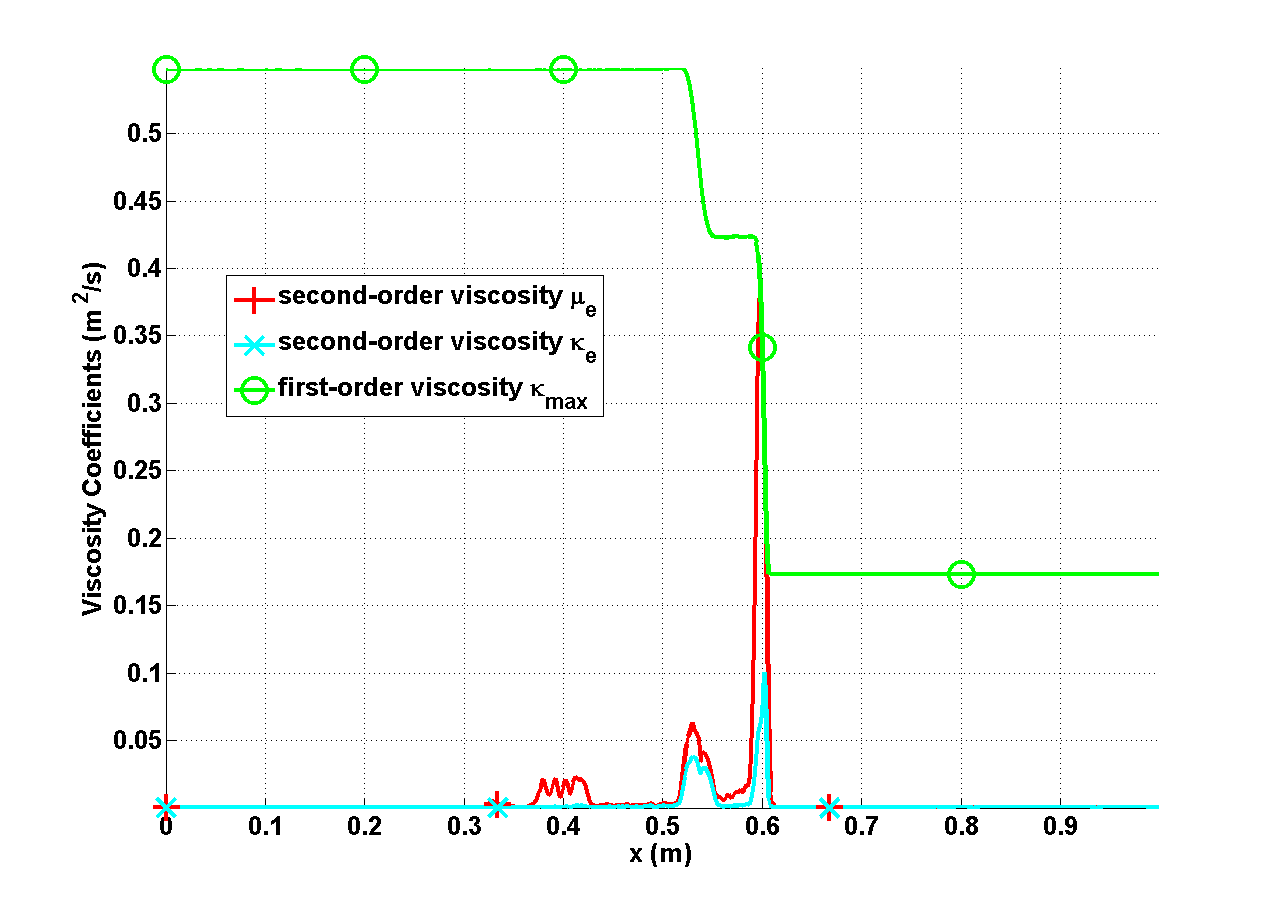
\includegraphics[width=\textwidth]{../figures/SEM/two_phases_vapor_viscosity_kappa_mu.png}
                \caption{Viscosity coefficients phase $2$}
        \end{subfigure}%
\end{figure}
\begin{figure}[H]        
\centering
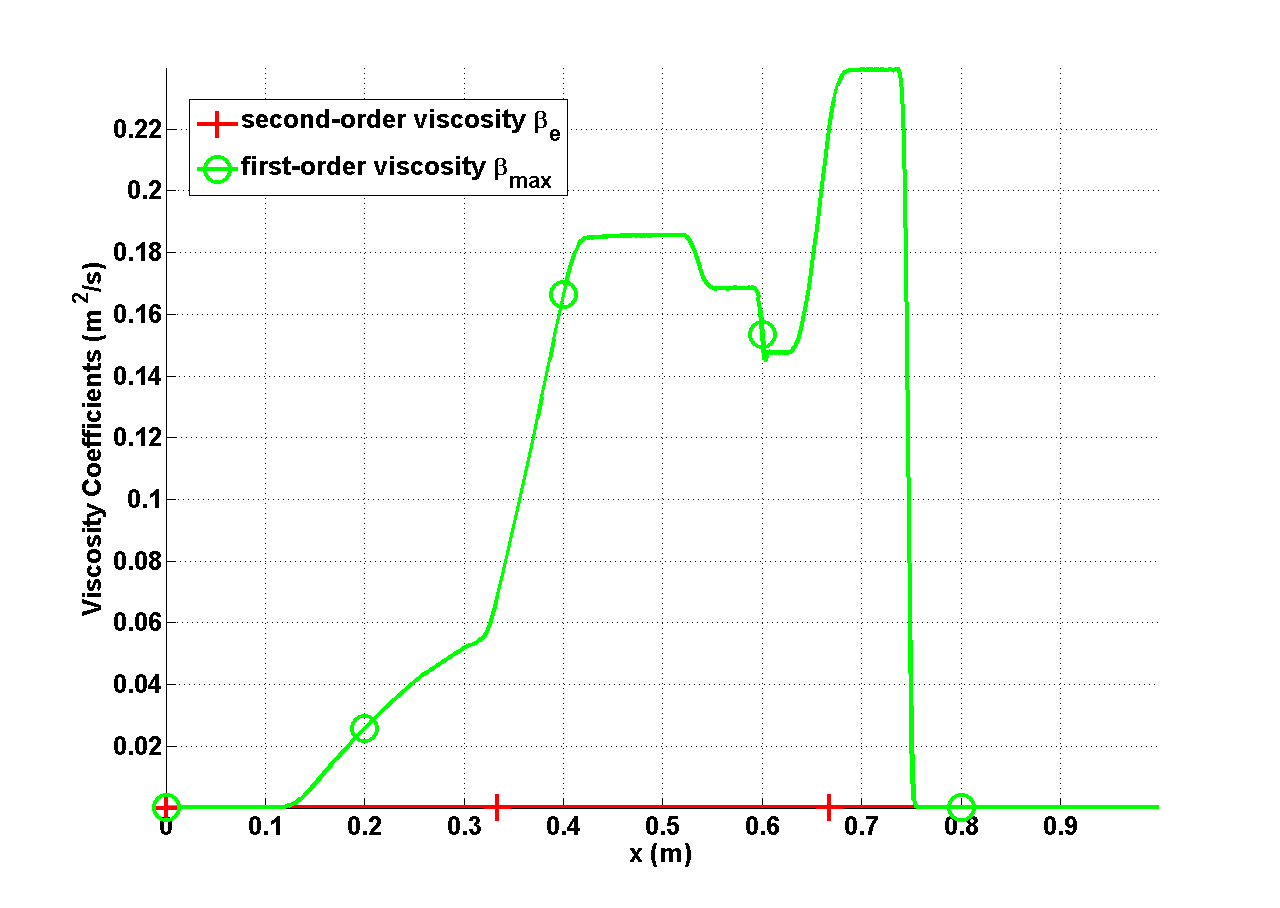
\includegraphics[width=0.37\textwidth]{../figures/SEM/two_phases_liquid_beta.png}
\caption{Viscosity coefficients volume fraction}
\end{figure}
\end{frame}
%************************************************
\begin{frame}{$1$-D shock tube with infinite relaxation coefficients}
\begin{block}{}
\begin{itemize}
\setlength{\itemsep}{5pt}
\item same fluids, same initial conditions and same equation of state
\item relaxation parameters are turned on and computed with $A_{int,max} = 10^4 m^{-1}$
\begin{align}
\mu_p = \frac{A_{int}}{Z_1+Z_2} \nonumber \\
\lambda_u = \frac{\mu_P}{2} Z_1 Z_2 \nonumber \\
A_{int} = A_{int,max} \nonumber
\end{align}
\item volume fraction will vary because of the pressure relaxation term
\item NO exact solution available
\end{itemize}
\end{block}
Objective: verify that the volume fraction is correctly stabilized by the EVM
\end{frame}
%************************************************
\begin{frame}{$1$-D shock tube with infinite relaxation coefficients}
\begin{figure}
        \begin{subfigure}[b]{0.37\textwidth}
                \centering
                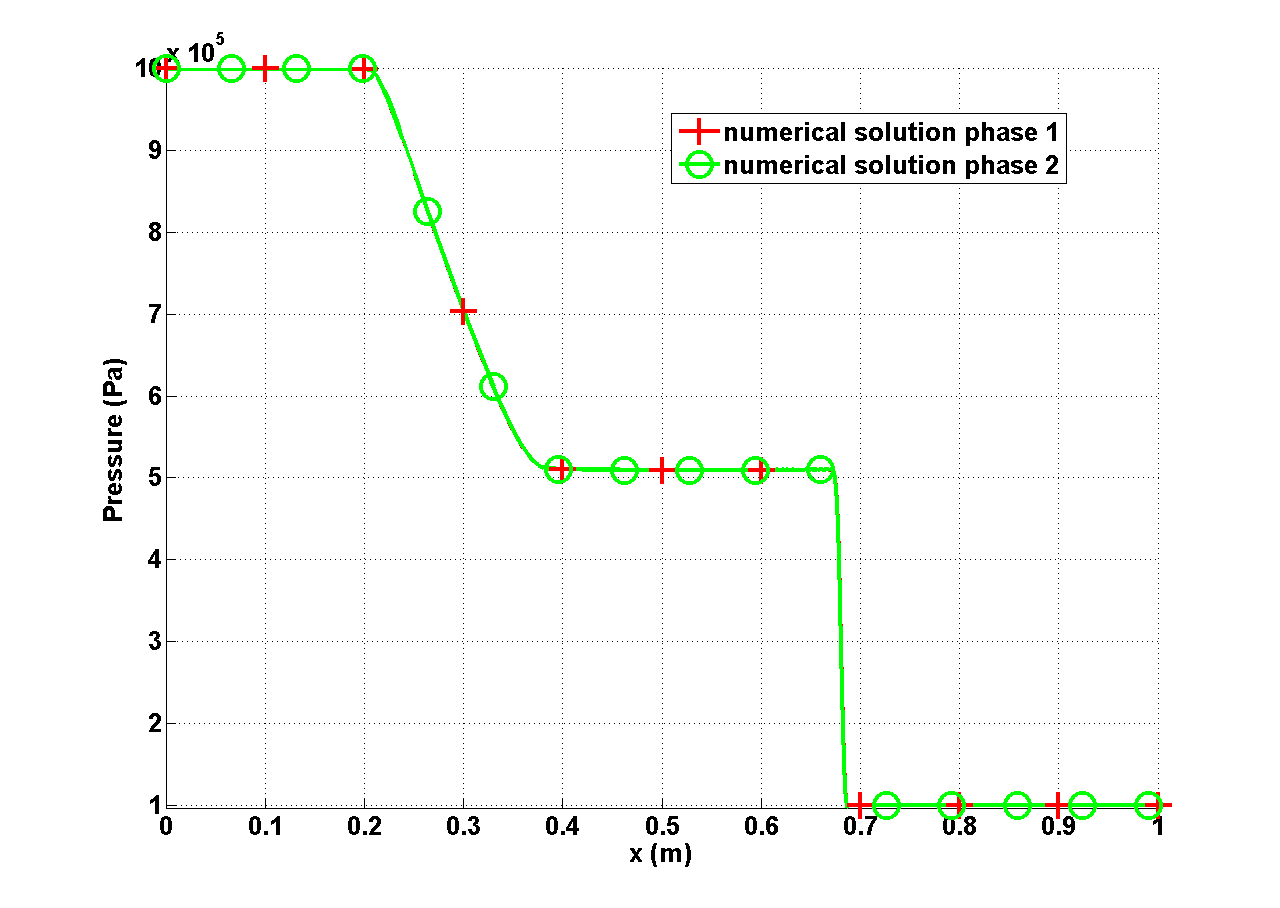
\includegraphics[width=\textwidth]{../figures/SEM/relaxation_two_phases_pressure.png}
                \caption{Pressure at $t=305$ $\mu s$}
        \end{subfigure}%
        \begin{subfigure}[b]{0.37\textwidth}
                \centering
                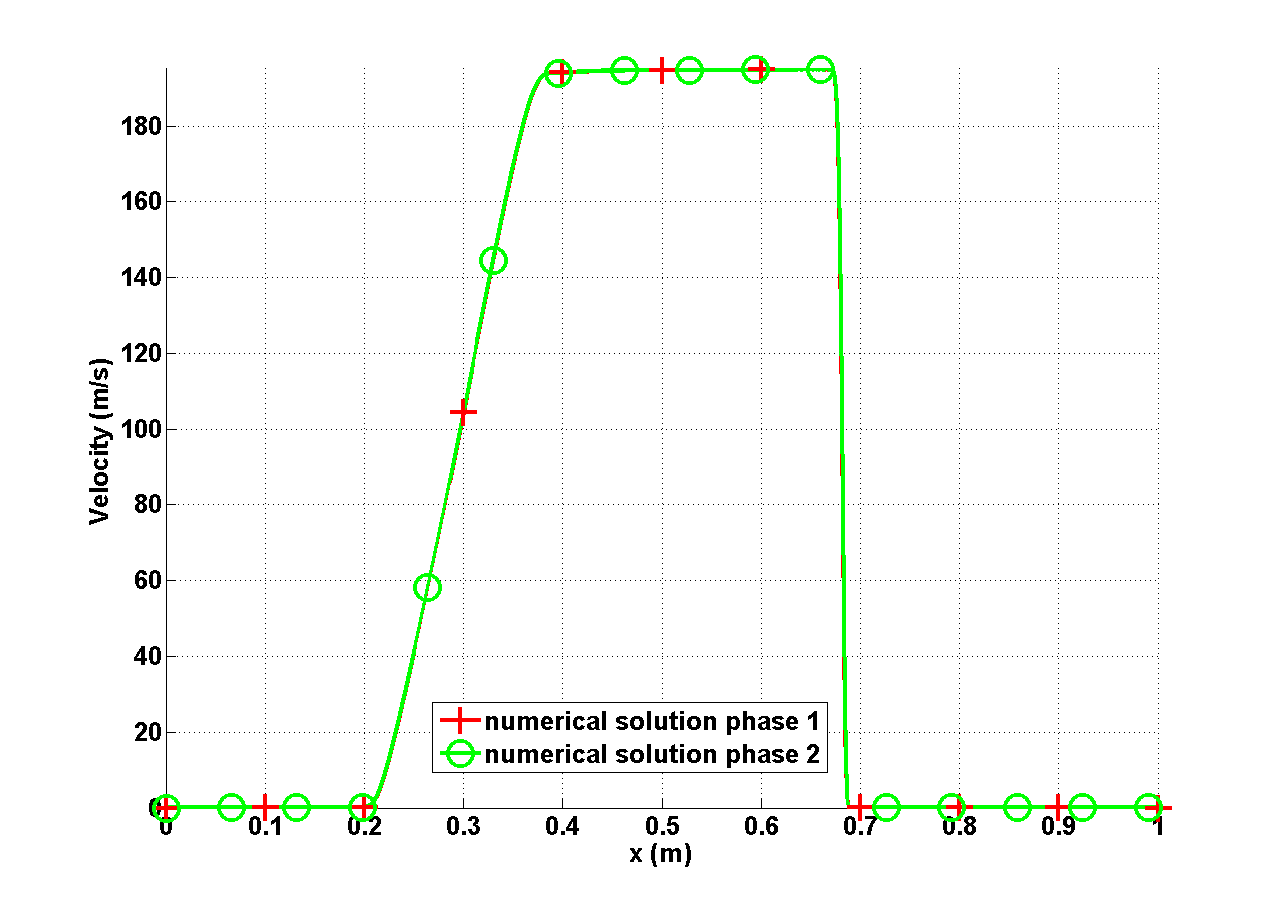
\includegraphics[width=\textwidth]{../figures/SEM/relaxation_two_phases_velocity.png}
                \caption{Velocity at $t=305$ $\mu s$}
        \end{subfigure}%

        \begin{subfigure}[b]{0.37\textwidth}
                \centering
                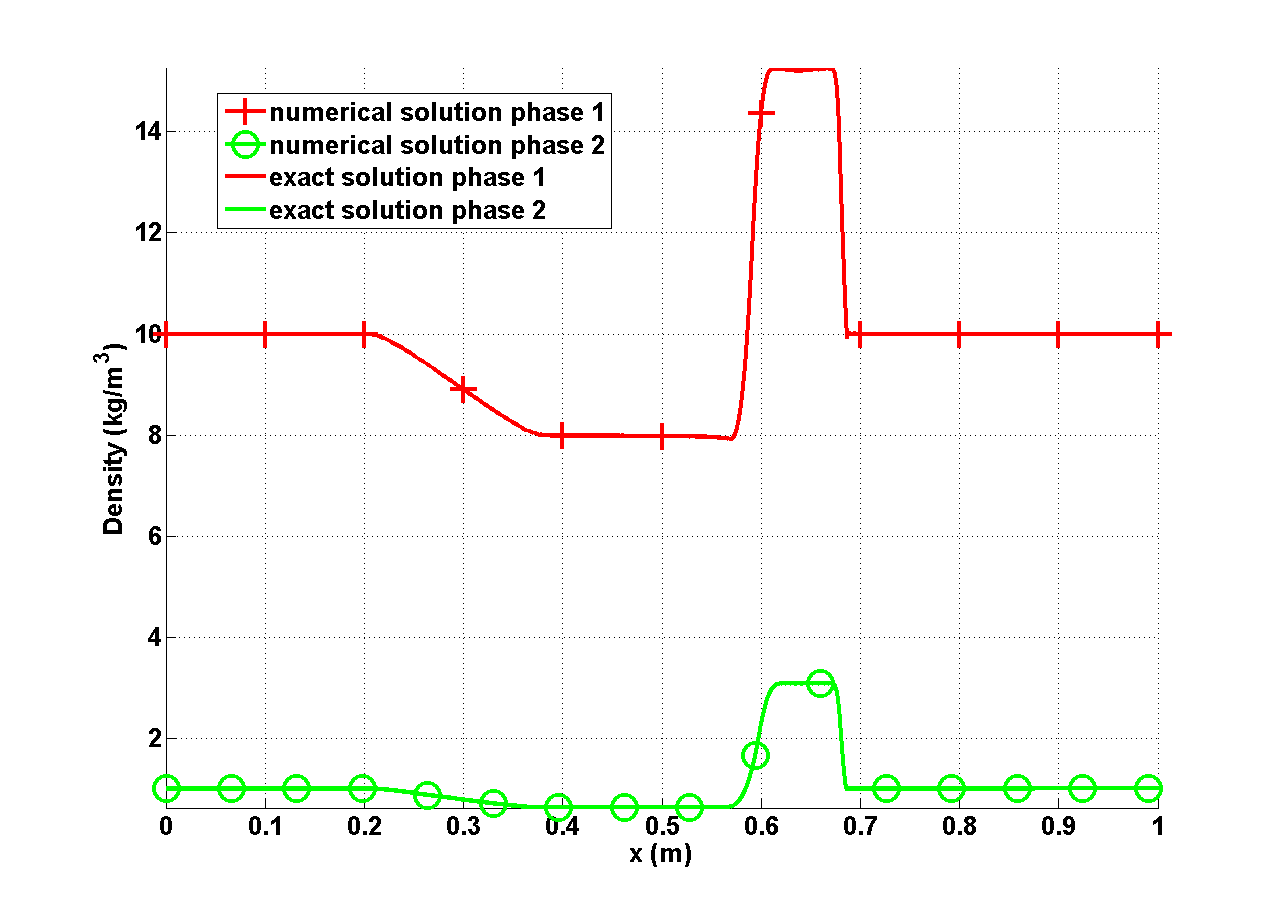
\includegraphics[width=\textwidth]{../figures/SEM/relaxation_two_phases_density.png}
                \caption{Pressure at $t=305$ $\mu s$}
        \end{subfigure}%
        \begin{subfigure}[b]{0.37\textwidth}
                \centering
                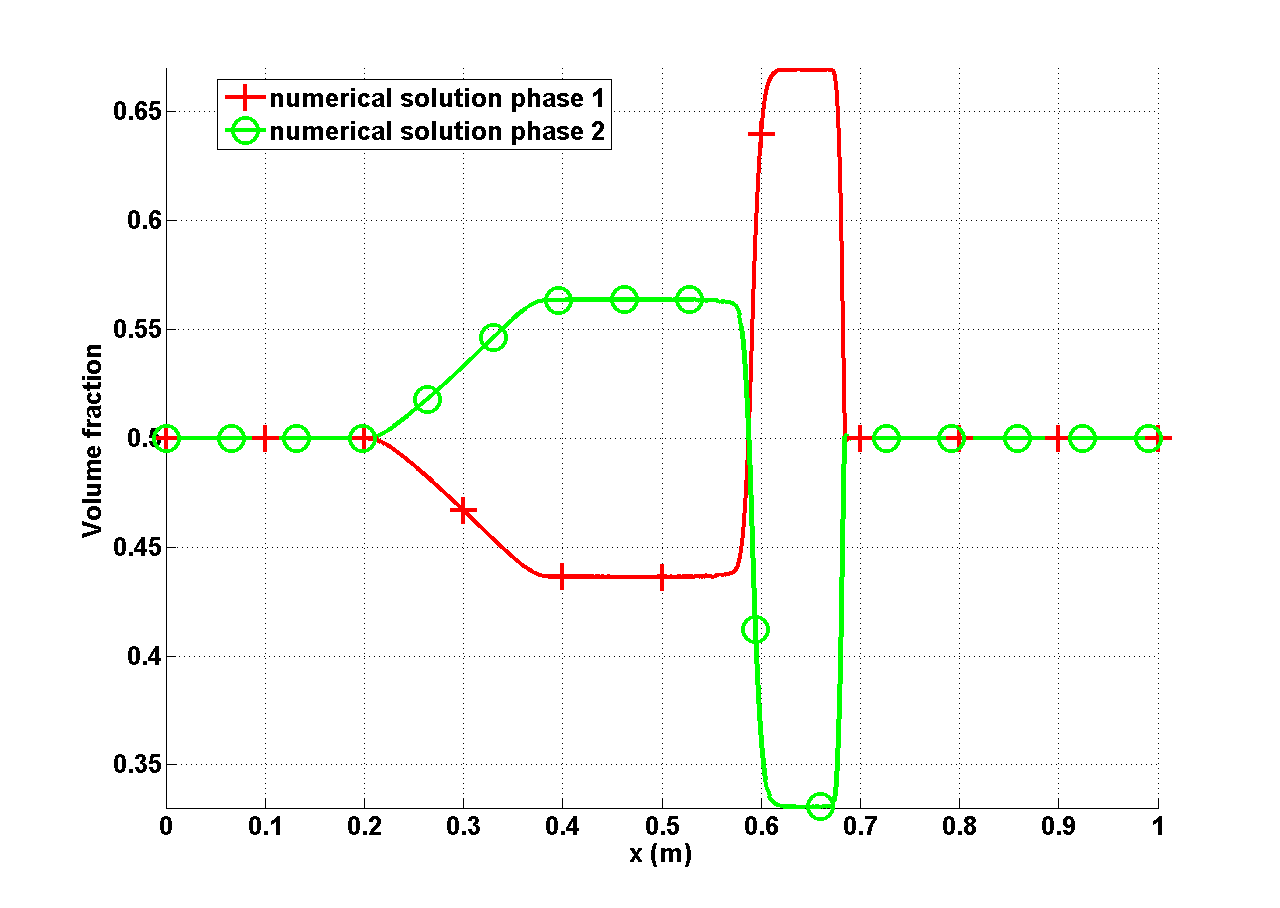
\includegraphics[width=\textwidth]{../figures/SEM/relaxation_two_phases_volume_fraction.png}
                \caption{Velocity at $t=305$ $\mu s$}
        \end{subfigure}%
\end{figure}
\end{frame}
%************************************************
\begin{frame}{$1$-D shock tube with infinite relaxation coefficients}
\begin{figure}
        \begin{subfigure}[b]{0.37\textwidth}
                \centering
                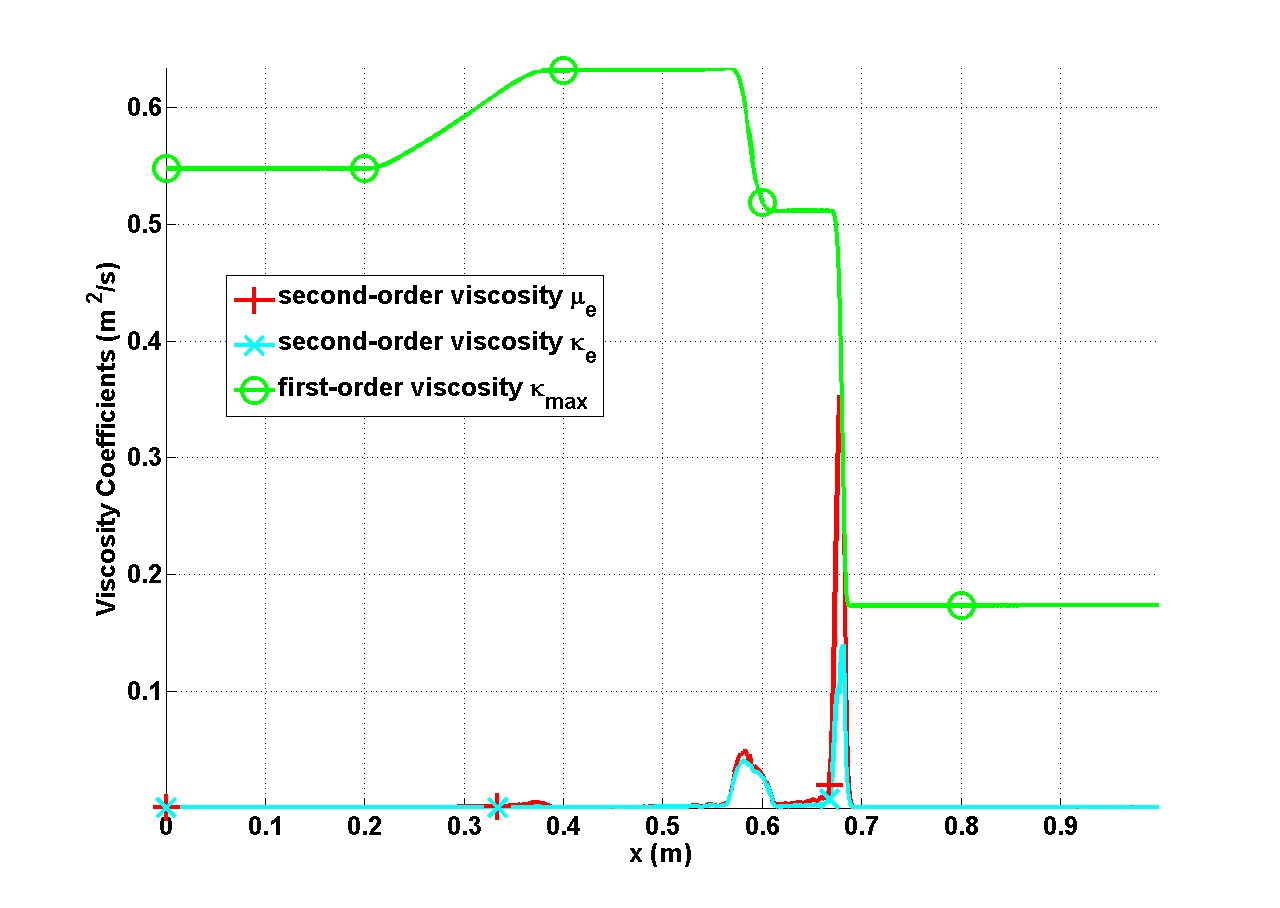
\includegraphics[width=\textwidth]{../figures/SEM/relaxation_two_phases_liquid_viscosity_kappa_mu.png}
                \caption{Viscosity coefficients phase $1$}
        \end{subfigure}%
        \begin{subfigure}[b]{0.37\textwidth}
                \centering
                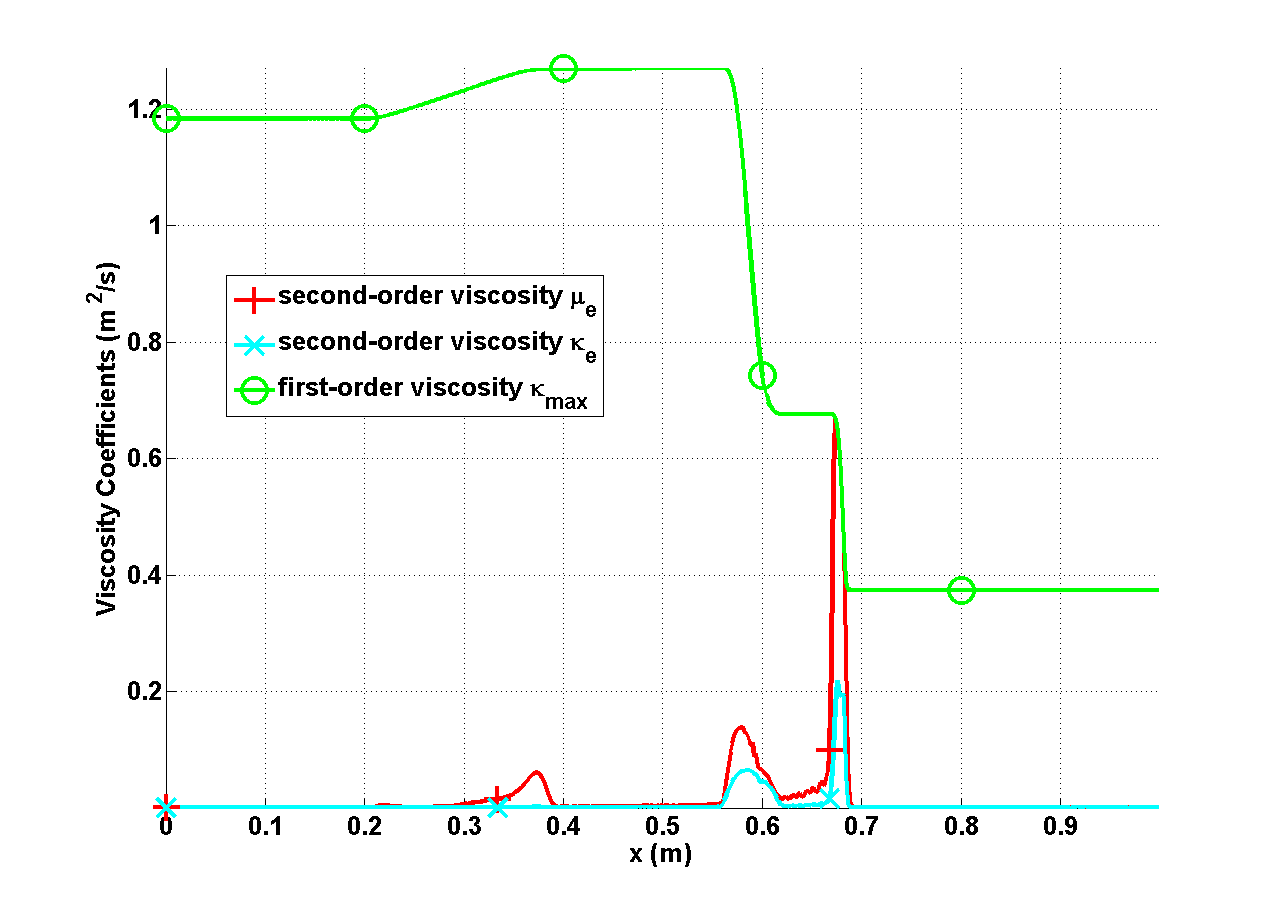
\includegraphics[width=\textwidth]{../figures/SEM/relaxation_two_phases_vapor_viscosity_kappa_mu.png}
                \caption{Viscosity coefficients phase $2$}
        \end{subfigure}%
\end{figure}
\begin{figure}[H]        
\centering
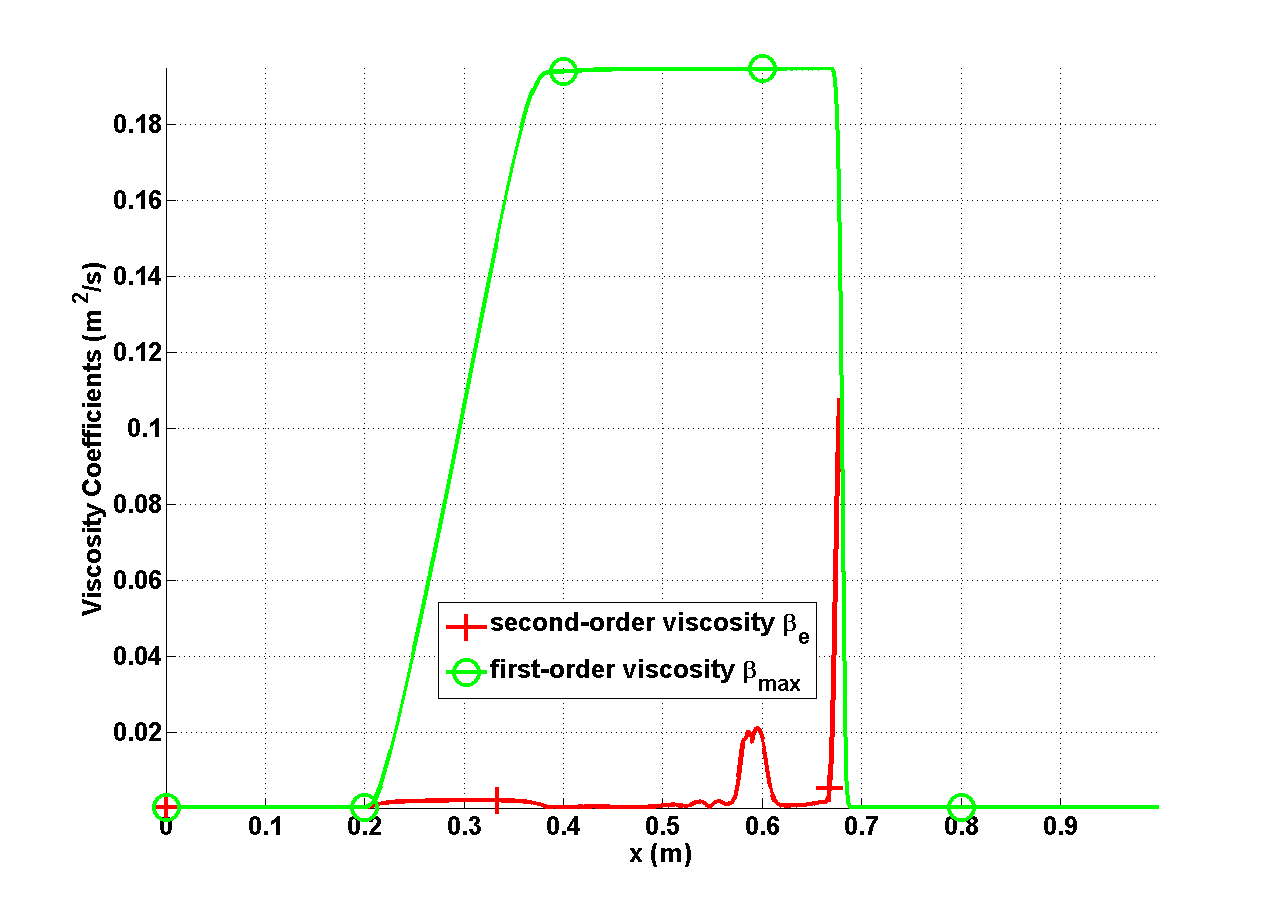
\includegraphics[width=0.37\textwidth]{../figures/SEM/relaxation_two_phases_liquid_beta.png}
\caption{Viscosity coefficients volume fraction}
\end{figure}
\end{frame}
%************************************************
\section{Conclusions and future work}
\begin{frame}{Conclusions and future work}
\begin{block}{The multi-D Euler equations with variable area}
\begin{itemize}
\item extended the viscous regularization to Euler equation with variable area
\item extended the EVM to low-Mach flows by doing a low-Mach asymptotic limit $\rightarrow$ worked with non-dimensionalized equations
\item validated our approach with $1$ and $2$-D simulations and convergence tests
\item applied the EVM with the Stiffened Gas equation of state
\end{itemize}
\end{block}
\begin{block}{The seven equation model (SEM)}
\begin{itemize}
\item derived a viscous regularization for the SEM
\item defined the viscosity coefficients using the same methodology as for single-phase flow equation
\item our approach was validated by $1$-D results
\end{itemize}
\end{block}
\begin{block}{Future work}
Use the viscous regularization for the SEM to run $2$-D simulations $\to$ require a preconditioner
\end{block}
\end{frame}
%************************************************
\begin{frame}{}
\begin{center}
The $1$-D Radiation-Hydrodynamic EquAtion \\
(RHEA)
\end{center}
\begin{figure}[H]
\centering
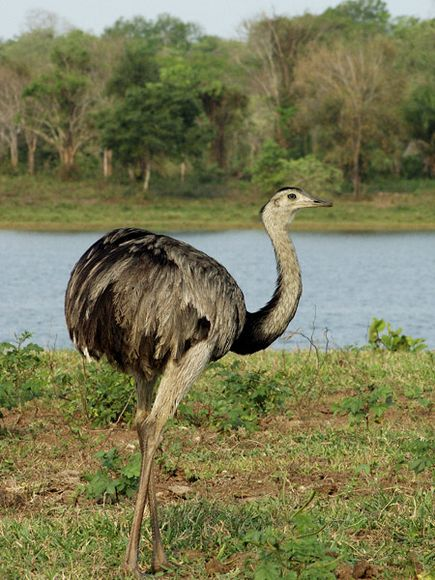
\includegraphics[width=0.45\textwidth]{../figures/rhea.png}
\end{figure}
\end{frame}
%************************************************
\begin{frame}{}
\begin{center}
\LARGE{\textbf{QUESTIONS/COMMENTS ?}}
\end{center}
\end{frame}
%************************************************
%************************************************
%************************************************
%************************************************
%************************************************
%************************************************
%************************************************
%************************************************
%************************************************
\begin{frame}{}
\begin{center}
$1$-D Euler equations numerical results
\end{center}
\end{frame}
%************************************************
\begin{frame}{Leblanc shock tube}
\begin{figure}[H]
        \centering
        \begin{subfigure}[b]{0.37\textwidth}
                \centering
                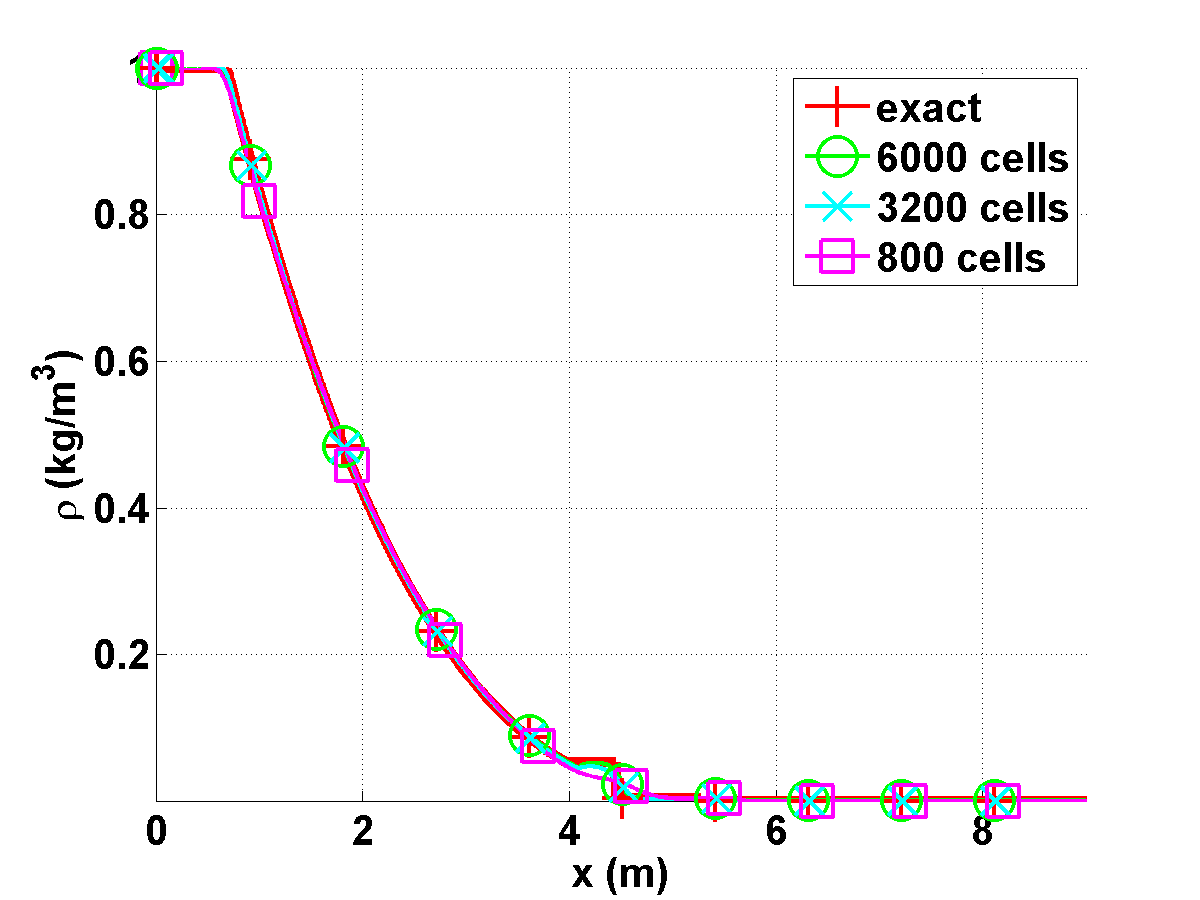
\includegraphics[width=\textwidth]{../figures/Leblanc_exact_and_numerical_stt_density_6000.png}
                \caption{Density}
        \end{subfigure}%
        %add desired spacing between images, e. g. ~, \quad, \qquad etc. 
          %(or a blank line to force the subfigure onto a new line)
        \begin{subfigure}[b]{0.37\textwidth}
                \centering
                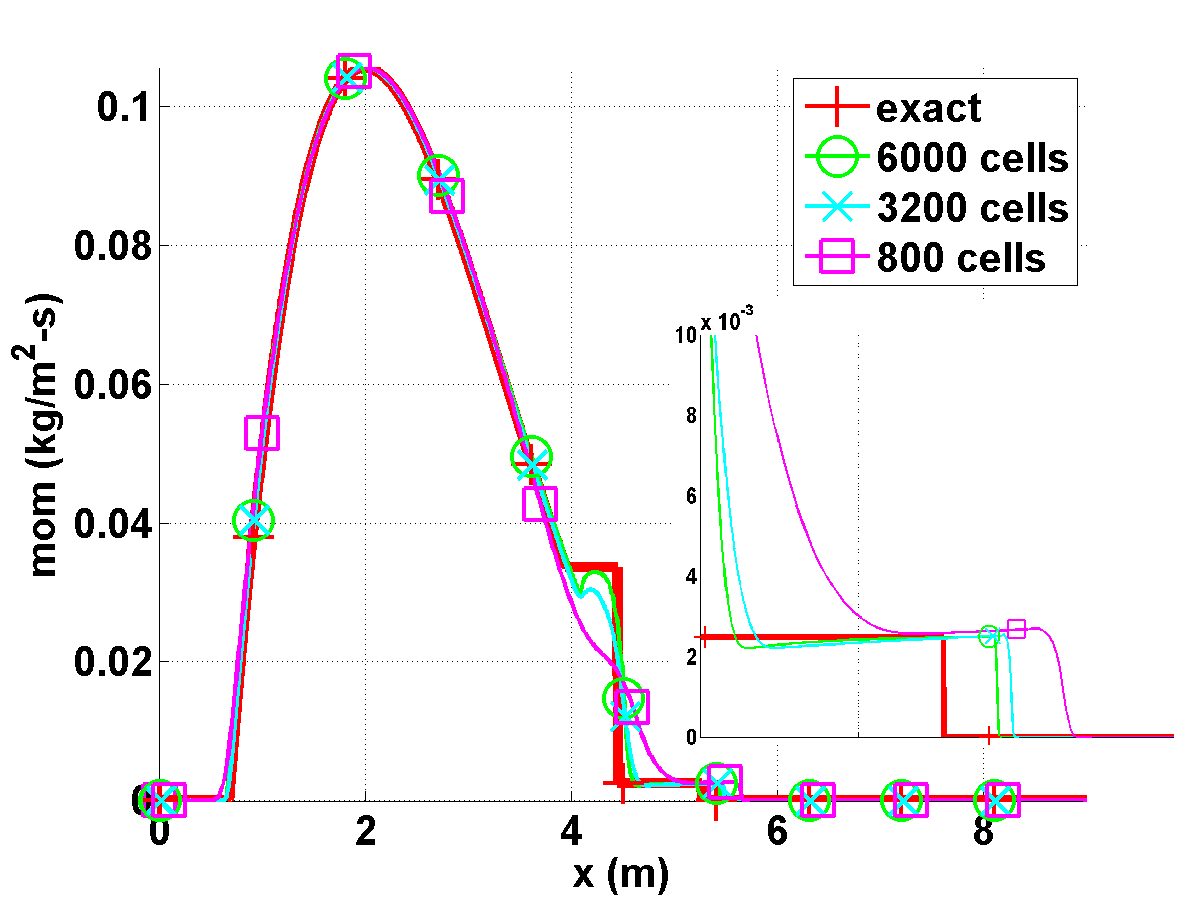
\includegraphics[width=\textwidth]{../figures/Leblanc_exact_and_numerical_stt_momentum_6000.png}
                \caption{Momentum}
        \end{subfigure}

        \begin{subfigure}[b]{0.37\textwidth}
                \centering
                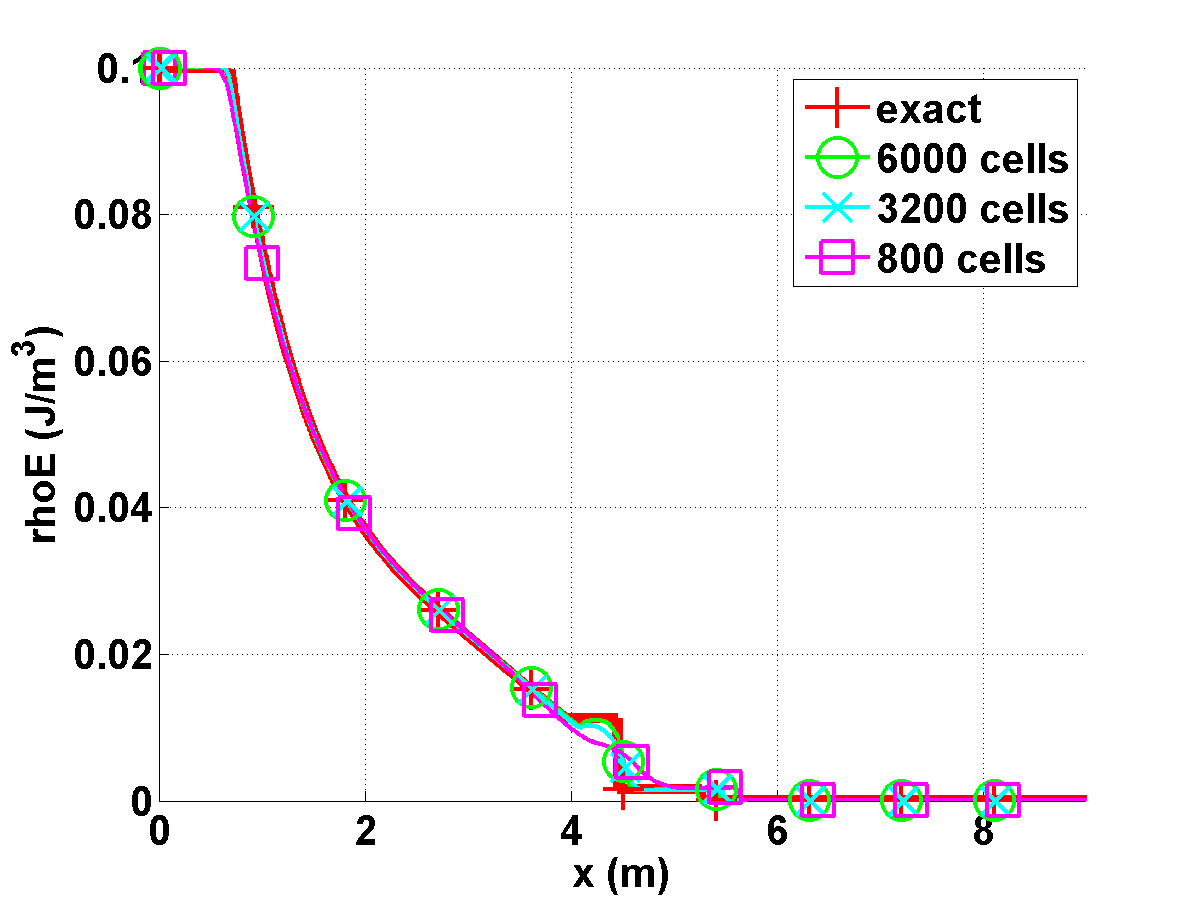
\includegraphics[width=\textwidth]{../figures/Leblanc_exact_and_numerical_stt_total_energy_6000.png}
                \caption{Total energy}
        \end{subfigure}
          %add desired spacing between images, e. g. ~, \quad, \qquad etc. 
          %(or a blank line to force the subfigure onto a new line)
        \begin{subfigure}[b]{0.37\textwidth}
                \centering
                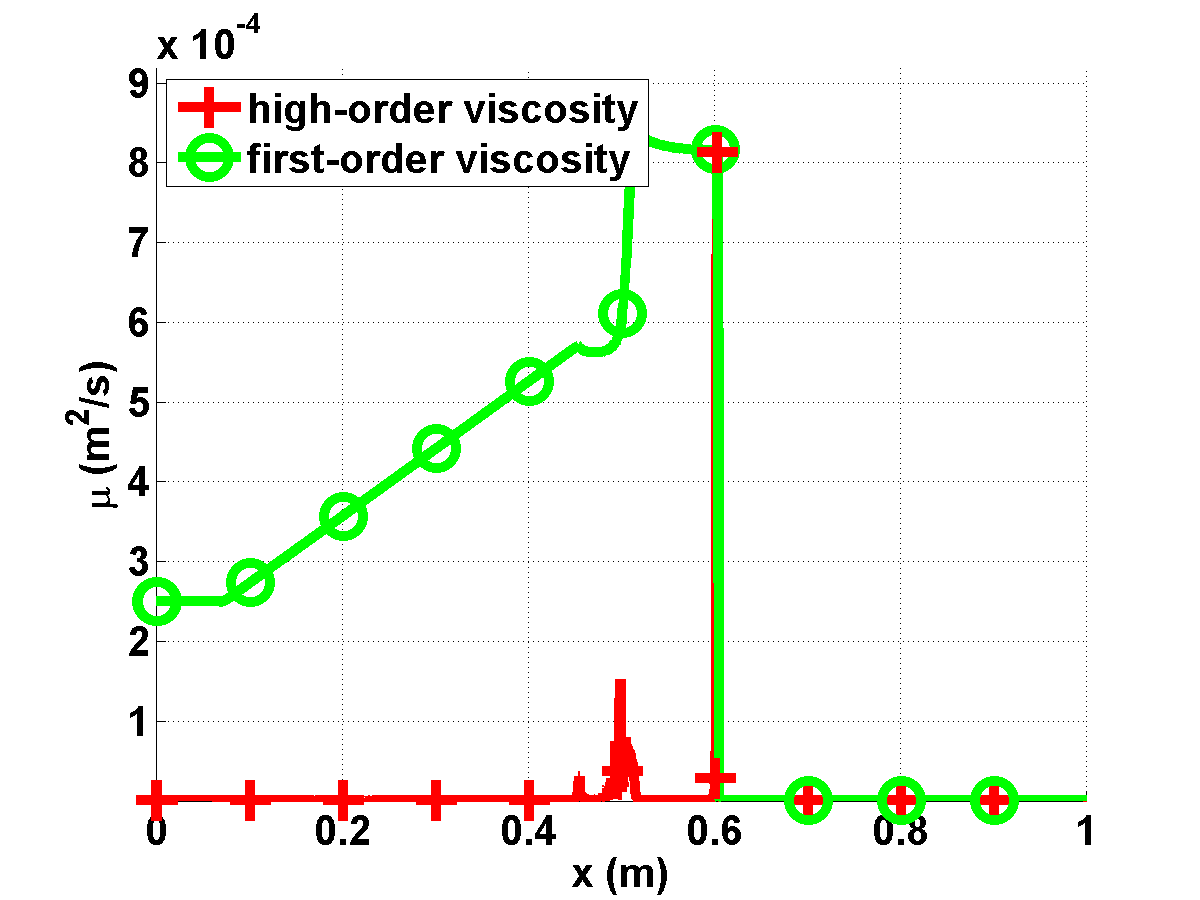
\includegraphics[width=\textwidth]{../figures/Leblanc_viscosity_numerical_6000.png}
                \caption{Viscosity coefficients}
        \end{subfigure}
\end{figure}
\end{frame}
%************************************************
\begin{frame}{Shock tube for liquid phase}
\begin{figure}[H]
        \centering
        \begin{subfigure}[b]{0.5\textwidth}
                \centering
                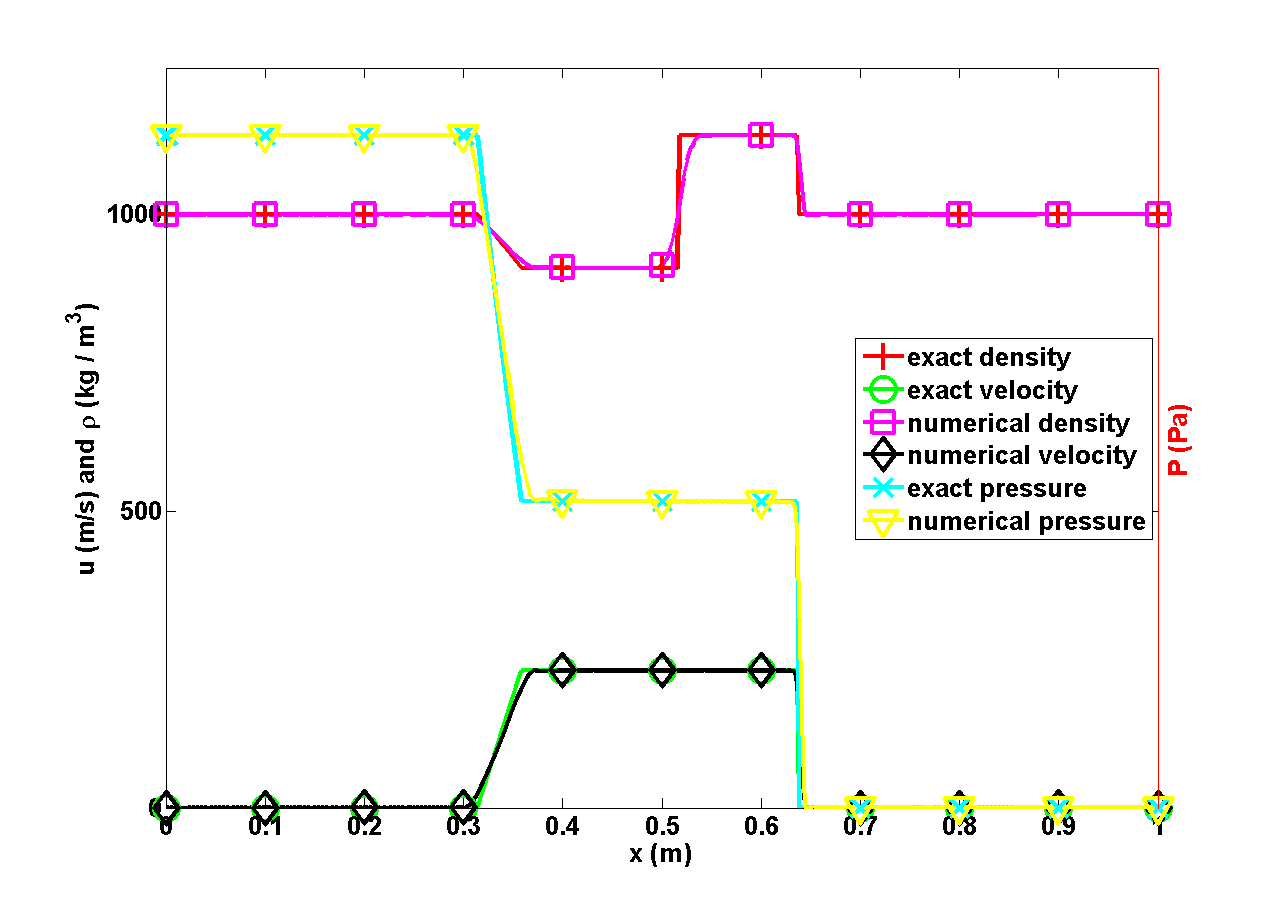
\includegraphics[width=\textwidth]{../figures/LiquidSrongShock_density_velocity_pressure_profiles.png}
                \caption{Density, velocity and pressure profiles.}
        \end{subfigure}%
        \begin{subfigure}[b]{0.5\textwidth}
                \centering
                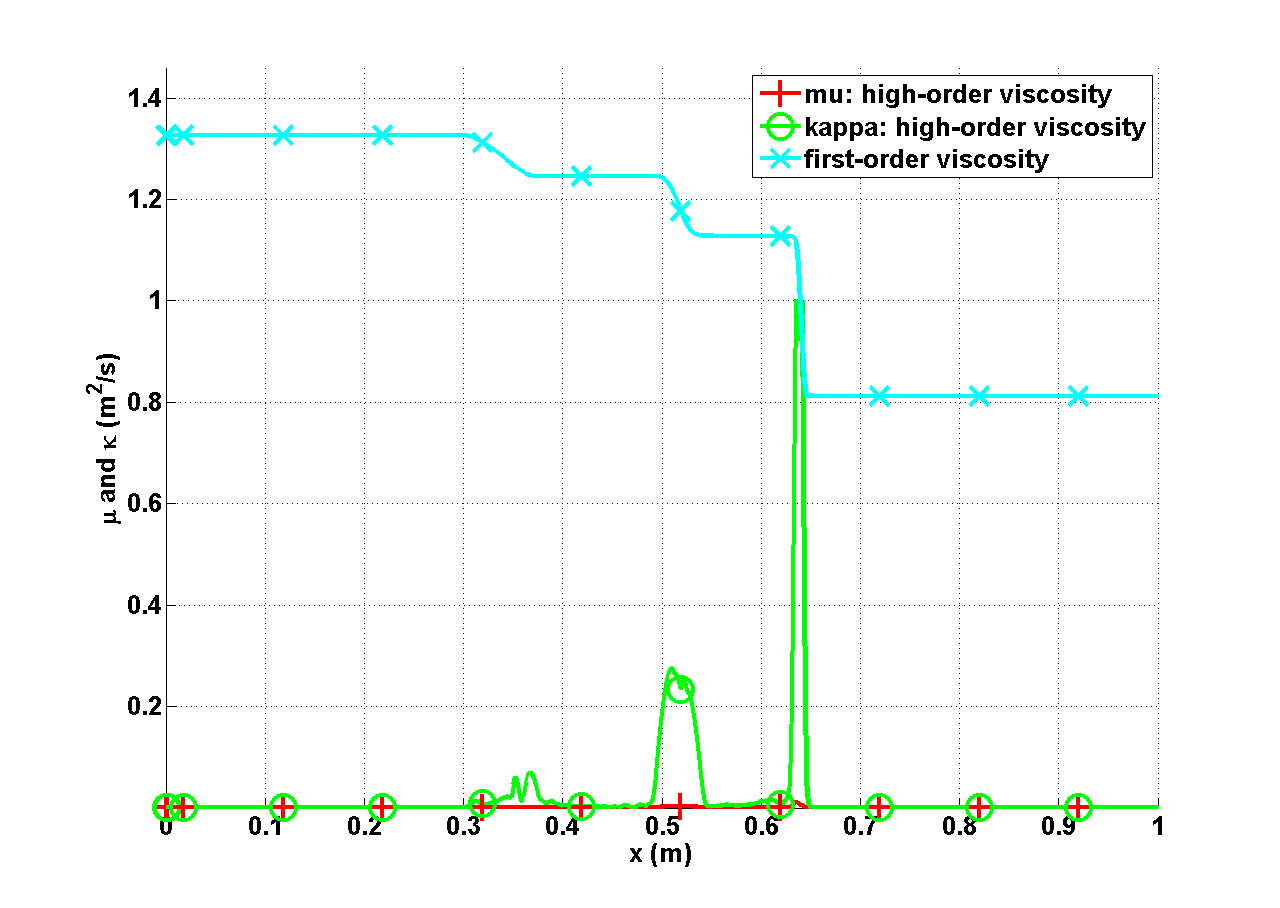
\includegraphics[width=\textwidth]{../figures/LiquidSrongShock_viscosity.png}
                \caption{Viscosity coefficients profile.}
        \end{subfigure}
\end{figure}
\end{frame}
%************************************************
\begin{frame}{Slow moving shock}
\begin{figure}[H]
        \centering
        \begin{subfigure}[b]{0.5\textwidth}
                \centering
                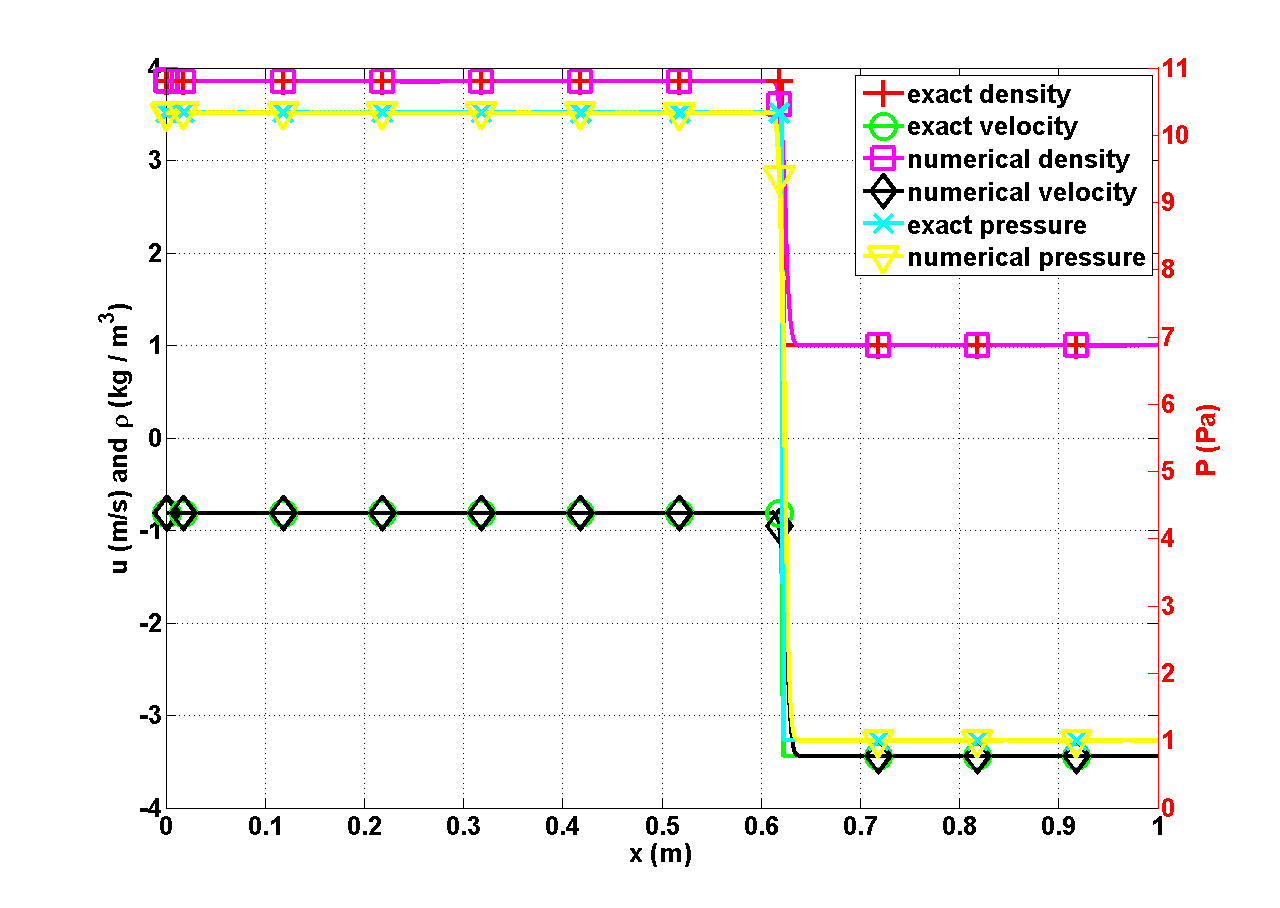
\includegraphics[width=\textwidth]{../figures/SlowMovingShock_density_velocity_pressure_profiles.png}
                \caption{Velocity, density and pressure}
        \end{subfigure}%
        \begin{subfigure}[b]{0.5\textwidth}
                \centering
                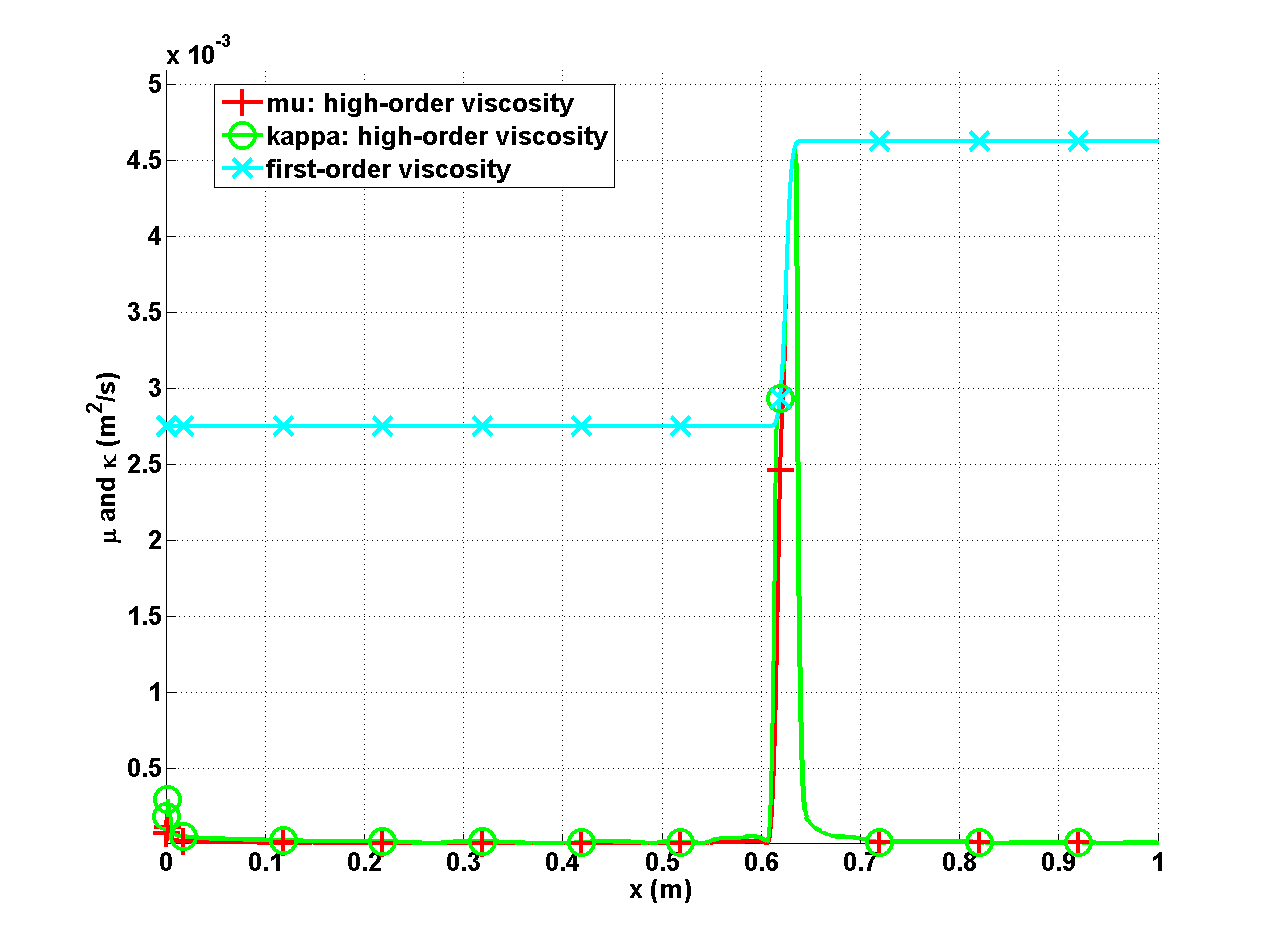
\includegraphics[width=\textwidth]{../figures/SlowMovingShock_viscosity.png}
                \caption{Viscosity coefficients}
        \end{subfigure} 
\end{figure} 
\end{frame}
%************************************************
\begin{frame}{PWR}
\begin{figure}[H]
\begin{subfigure}[b]{0.37\textwidth}
\centering
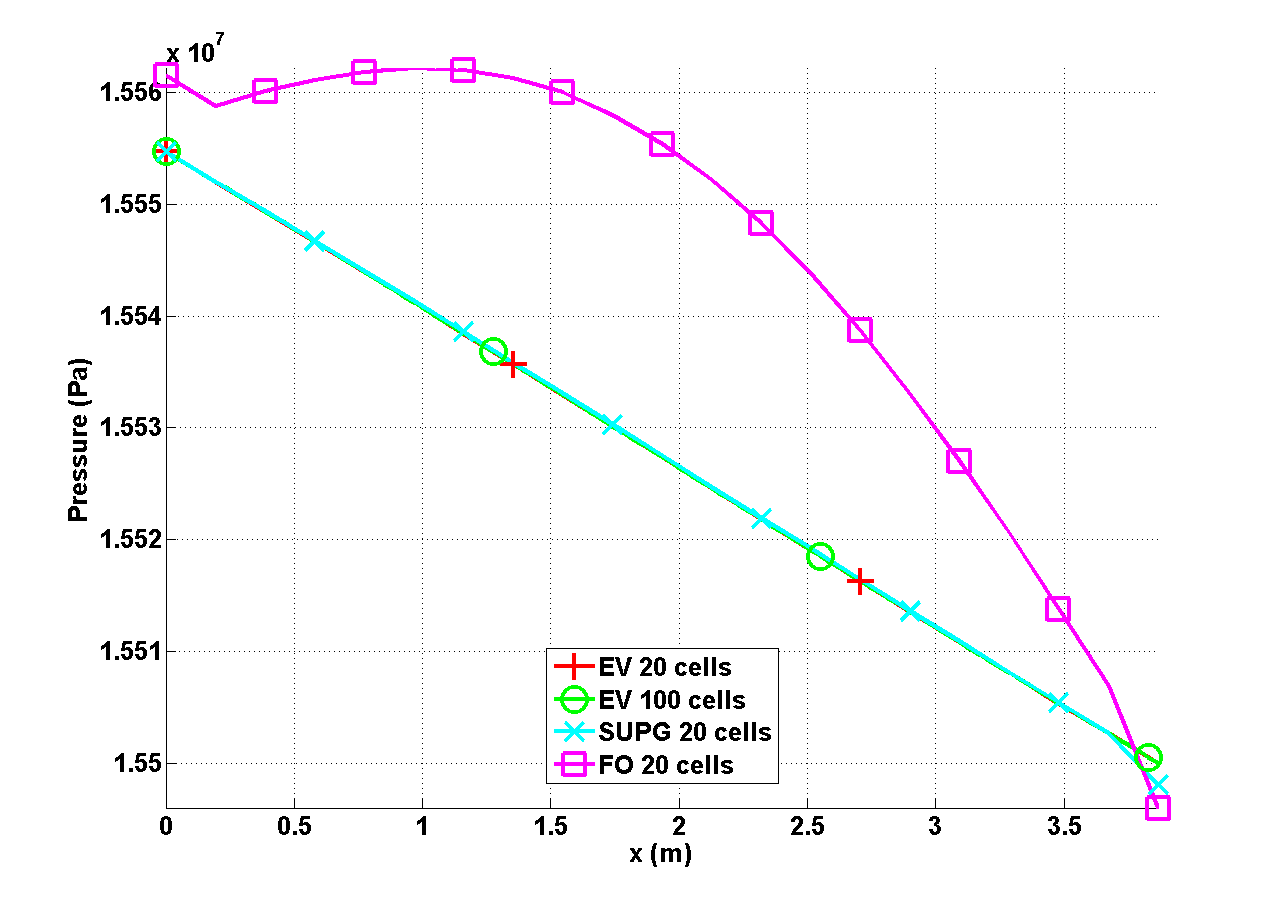
\includegraphics[width=\textwidth]{../figures/PWR_stt_pressure.png}
\caption{Axial pressure profile}
\end{subfigure}
%
\begin{subfigure}[b]{0.37\textwidth}
\centering
\includegraphics[width=\textwidth]{../figures/PWR_stt_temperature.png}
\caption{Axial temperature profile}
\end{subfigure}

\begin{subfigure}[b]{0.37\textwidth}
\centering
\includegraphics[width=\textwidth]{../figures/PWR_stt_velocity.png}
\caption{Axial velocity profile}
\end{subfigure}
%
\begin{subfigure}[b]{0.37\textwidth}
\centering
\includegraphics[width=\textwidth]{../figures/PWR_stt_viscosity.png}
\caption{Axial viscosity profile}
\end{subfigure}
\end{figure}
\end{frame}
%************************************************
\begin{frame}{}
\begin{center}
$2$-D Euler equations numerical results
\end{center}
\end{frame}
%************************************************
\begin{frame}{$2$-D explosion: solution at $t=0.2$ $s$}
\begin{figure}[H]
\begin{subfigure}[b]{0.45\textwidth}
\centering
\includegraphics[width=\textwidth]{../figures/Explosion_density_profiles.png}
\caption{Density}
\end{subfigure}
%
\begin{subfigure}[b]{0.45\textwidth}
\centering
\includegraphics[width=\textwidth]{../figures/Explosion_viscosity_profiles.png}
\caption{Viscosity coefficient}
\end{subfigure}
\end{figure}
\end{frame}
%************************************************
\begin{frame}{$2$-D compression corner}
  \begin{columns}
    \column{.5\textwidth}
       \includemedia[addresource=compression_corner.mp4, activate=pageopen, deactivate=pageclose, width=6.5cm, height=5cm, flashvars={source=compression_corner.mp4 & autoPlay=true & loop=true }]{}{VPlayer.swf}
    \column{.5\textwidth}
      \includemedia[addresource=compression_corner_viscosity.mp4, activate=pageopen, deactivate=pageclose, width=6.5cm, height=5cm, flashvars={source=compression_corner_viscosity.mp4 & autoPlay=true & loop=true }]{}{VPlayer.swf}
  \end{columns}
\end{frame}
%************************************************
\begin{frame}{Supersonic flow over a $5^\circ$ double-wedge obstruction}
\begin{figure}
\begin{subfigure}[b]{0.45\textwidth}
                \centering
                \includegraphics[width=\textwidth]{../figures/DWOMachNumberStt.png}
                \caption{Pressure }
        \end{subfigure}
\begin{subfigure}[b]{0.45\textwidth}
                \centering
                \includegraphics[width=\textwidth]{../figures/DWOViscosityStt.png}
                \caption{Viscosity coefficient}
        \end{subfigure}
\end{figure}
\end{frame}
%************************************************
\begin{frame}
\begin{center}
Seven equation model
\end{center}
\end{frame}
%************************************************
\begin{frame}{$1$-D converging-diverging nozzle with relaxation terms}
\begin{figure}[H]
\begin{subfigure}[b]{0.38\textwidth}
\centering
\includegraphics[width=\textwidth]{../figures/SEM/Aint1e4_two_phases_pressure.png}
\caption{Pressure}
\end{subfigure}
%
\begin{subfigure}[b]{0.38\textwidth}
\centering
\includegraphics[width=\textwidth]{../figures/SEM/Aint1e4_two_phases_velocity.png}
\caption{Velocity}
\end{subfigure}

\begin{subfigure}[b]{0.38\textwidth}
\centering
\includegraphics[width=\textwidth]{../figures/SEM/Aint1e4_two_phases_density.png}
\caption{Density}
\end{subfigure}
%
\begin{subfigure}[b]{0.38\textwidth}
\centering
\includegraphics[width=\textwidth]{../figures/SEM/Aint1e4_two_phases_volume_fraction.png}
\caption{Volume fraction}
\end{subfigure}
\end{figure}
\end{frame}
%************************************************
\begin{frame}{$1$-D converging-diverging nozzle with relaxation terms}
\begin{figure}[H]
\begin{subfigure}[b]{0.38\textwidth}
\centering
\includegraphics[width=\textwidth]{../figures/SEM/Aint1e4_liquid_viscosity_kappa_mu.png}
\caption{Liquid water}
\end{subfigure}
%
\begin{subfigure}[b]{0.38\textwidth}
\centering
\includegraphics[width=\textwidth]{../figures/SEM/Aint1e4_vapor_viscosity_kappa_mu.png}
\caption{Vapor}
\end{subfigure}

\begin{subfigure}[b]{0.38\textwidth}
\centering
\includegraphics[width=\textwidth]{../figures/SEM/Aint1e4_liquid_beta.png}
\caption{$\beta$}
\end{subfigure}
\end{figure}
\end{frame}
%************************************************
\begin{frame}{$1$-D converging-diverging nozzle with all source terms}
\begin{figure}[H]
\begin{subfigure}[b]{0.37\textwidth}
\centering
\includegraphics[width=\textwidth]{../figures/SEM/Aint1e3MassOn_two_phases_pressure.png}
\caption{Pressure}
\end{subfigure}
%
\begin{subfigure}[b]{0.37\textwidth}
\centering
\includegraphics[width=\textwidth]{../figures/SEM/Aint1e3MassOn_two_phases_velocity.png}
\caption{Velocity}
\end{subfigure}

\begin{subfigure}[b]{0.37\textwidth}
\centering
\includegraphics[width=\textwidth]{../figures/SEM/Aint1e3MassOn_two_phases_density.png}
\caption{Density}
\end{subfigure}
%
\begin{subfigure}[b]{0.37\textwidth}
\centering
\includegraphics[width=\textwidth]{../figures/SEM/Aint1e3MassOn_two_phases_volume_fraction.png}
\caption{Volume fraction}
\end{subfigure}
\end{figure}
\end{frame}
%************************************************
\begin{frame}{$1$-D converging-diverging nozzle with all source terms}
\begin{figure}[H]
\begin{subfigure}[b]{0.38\textwidth}
\centering
\includegraphics[width=\textwidth]{../figures/SEM/Aint1e4_liquid_viscosity_kappa_mu.png}
\caption{Liquid water}
\end{subfigure}
%
\begin{subfigure}[b]{0.38\textwidth}
\centering
\includegraphics[width=\textwidth]{../figures/SEM/Aint1e4_vapor_viscosity_kappa_mu.png}
\caption{Vapor}
\end{subfigure}
\end{figure}
\begin{figure}
\centering
\includegraphics[width=0.38\textwidth]{../figures/SEM/Aint1e4_liquid_beta.png}
\caption{$\beta$}
\end{figure}
\end{frame}
%************************************************
\begin{frame}
\begin{center}
$1$-D Grey Radiation-Hydrodynamic equations
\end{center}
\end{frame}
%************************************************
\begin{frame}{Equations}
\begin{block}{}
\begin{align}
&\partial_t \left( \rho \right) + \partial_x\left( \rho u \right) = \partial_x \left( \kappa \partial_x \rho \right) \nonumber \\
&\partial_t \left( \rho u\right) + \partial_x \left(\rho u^2 + P + \frac{\epsilon}{3} \right) = \partial_x \left( \kappa \partial_x \rho u \right) \nonumber \\
&\partial_t \left( \rho E\right) + \partial_x \left[ u \left( \rho E + P \right) \right] + \frac{u}{3} \partial_x \epsilon = \partial_x \left( \kappa \partial_x(\rho E) \right) \nonumber \\
&\partial_t \epsilon + \frac{4}{3} \partial_x \left( u \epsilon \right) - \frac{u}{3} \partial_x \epsilon = \partial_x \left( \kappa \partial_x \epsilon \right) \nonumber 
\end{align}
\end{block}
\end{frame}
%************************************************
\begin{frame}{Steady-state solution for Mach $1.05$}
\begin{figure}
\begin{subfigure}[b]{0.35\textwidth}
                \centering
                \includegraphics[width=\textwidth]{../figures/Mach_1p05_nel_500_temperature.png}
        \caption{Temperatures.}
\end{subfigure}
\begin{subfigure}[b]{0.35\textwidth}
                \centering
                \includegraphics[width=\textwidth]{../figures/Mach_1p05_nel_500_density}
        \caption{Material density.}
\end{subfigure}
\end{figure}

\begin{figure}
                \centering
                \includegraphics[width=0.35\textwidth]{../figures/Mach_1p05_nel_500_viscosity.png}
        \caption{Viscosity coefficients}
\end{figure}
\end{frame}
%************************************************
\begin{frame}{Steady-state solution for Mach $2$}
\begin{figure}
\begin{subfigure}[b]{0.35\textwidth}
                \centering
                \includegraphics[width=\textwidth]{../figures/Mach_2_nel_2000_temperature.png}
        \caption{Temperatures.}
\end{subfigure}
\begin{subfigure}[b]{0.35\textwidth}
                \centering
                \includegraphics[width=\textwidth]{../figures/Mach_2_nel_2000_density.png}
        \caption{Material density.}
\end{subfigure}
\end{figure}

\begin{figure}
                \centering
                \includegraphics[width=0.35\textwidth]{../figures/Mach_2_nel_2000_viscosity.png}
        \caption{Viscosity coefficients}
\end{figure}
\end{frame}
%************************************************
\begin{frame}{Steady-state solution for Mach $5$}
\begin{figure}
\begin{subfigure}[b]{0.35\textwidth}
                \centering
                \includegraphics[width=\textwidth]{../figures/Mach_5_nel_1000_temperature.png}
        \caption{Temperatures.}
\end{subfigure}
\begin{subfigure}[b]{0.35\textwidth}
                \centering
                \includegraphics[width=\textwidth]{../figures/Mach_5_nel_2000_density.png}
        \caption{Material density.}
\end{subfigure}

\begin{subfigure}[b]{0.35\textwidth}
                \centering
                \includegraphics[width=\textwidth]{../figures/Mach_5_nel_2000_viscosity.png}
        \caption{Viscosity coefficients.}
\end{subfigure}
\begin{subfigure}[b]{0.35\textwidth}
                \centering
                \includegraphics[width=\textwidth]{../figures/Mach_5_comparison.png}
        \caption{Location of the peak.}
\end{subfigure}
\end{figure}

%\begin{figure}
%                \centering
%                \includegraphics[width=0.35\textwidth]{../figures/Mach_5_nel_2000_viscosity.png}
%        \caption{Viscosity coefficients}
%\end{figure}

\end{frame}
%************************************************
\begin{frame}{Steady-state solution for Mach $50$}
\begin{figure}
\begin{subfigure}[b]{0.35\textwidth}
                \centering
                \includegraphics[width=\textwidth]{../figures/Mach_50_nel_1000_temperature.png}
        \caption{Temperatures.}
\end{subfigure}
\begin{subfigure}[b]{0.35\textwidth}
                \centering
                \includegraphics[width=\textwidth]{../figures/Mach_50_nel_1000_density.png}
        \caption{Material density.}
\end{subfigure}
\end{figure}

\begin{figure}
                \centering
                \includegraphics[width=0.35\textwidth]{../figures/Mach_50_nel_1000_viscosity.png}
        \caption{Viscosity coefficients}
\end{figure}
\end{frame}
%************************************************
\end{document}